% spell-checker: disable
\documentclass[12pt]{report}

\usepackage[a4paper, margin=3cm]{geometry}
\usepackage[colorlinks]{hyperref}
\usepackage[justification=centering]{caption}
\usepackage[parfill]{parskip}
\usepackage[stable, bottom]{footmisc}
\usepackage[table, xcdraw, dvipsnames]{xcolor}
\usepackage[utf8]{inputenc}
\usepackage{adjustbox}
\usepackage{algorithm}
\usepackage{algpseudocode}
\usepackage{amsmath}
\usepackage{amssymb}
\usepackage{amsthm}
\usepackage{biblatex}
\usepackage{bm}
\usepackage{csquotes}
\usepackage{enumitem}
\usepackage{fancyhdr}
\usepackage{float}
\usepackage{graphicx}
\usepackage{listings}
\usepackage{multirow}
\usepackage{physics}
\usepackage{pslatex}
\usepackage{subcaption}
\usepackage{thmtools}
\usepackage{tikz}
\usepackage{url}

\MakeOuterQuote{"}

\bibliography{references.bib}
\BiblatexSplitbibDefernumbersWarningOff

\theoremstyle{definition}
\newtheorem{definition}{Definition}[chapter]

\def\chapterautorefname{Chapter}
\def\sectionautorefname{Section}
\def\subsectionautorefname{Section}
\def\subsubsectionautorefname{Section}
\newcommand{\algorithmautorefname}{Algorithm}

\renewcommand{\lstlistingname}{Code Sample}
\renewcommand{\lstlistlistingname}{List of Code Samples}

\renewcommand{\fbox}{\fcolorbox{lightgray}{white}}
\setlength{\fboxrule}{0.1pt}
\setlength{\fboxsep}{0pt}

\setcounter{secnumdepth}{3}

\immediate\write18{texcount -inc -sum -total -brief main.tex > word_count}

\hypersetup{
  linkcolor=Blue,
  citecolor=Blue,
  urlcolor=Blue
}

\lstdefinestyle{codestyle}{
  language=Python,
  numberstyle=\tiny\color{Gray},
  commentstyle=\color{Green},
  keywordstyle=\bfseries\color{Blue},
  stringstyle=\color{Maroon},
  basicstyle=\ttfamily,
  breakatwhitespace=false,
  breaklines=true,
  keepspaces=true, numbers=left, numbersep=5pt, showspaces=false,
  showstringspaces=false, showtabs=false, tabsize=2, frame=tb
}
\lstset{style=codestyle}

\begin{document}
\thispagestyle{empty}
\begin{center}
  \large
  
\includegraphics[width=0.4\linewidth]{figures/images/uom.png}
 \\
  \vspace*{0.4in}
  The University of Manchester \\
  Department of Computer Science \\
  April 2023 \\
  \vspace*{0.2in}
  \textbf{\LARGE{Exploring Model-Free Deep Reinforcement Learning Techniques for Racing Games}} \\
  \vspace*{0.2in}
  Author: Aryan Agrawal \\
  \vspace*{0.2in}
  Supervisor: Dr. Ke Chen
\end{center}
\begin{abstract}
  \begin{quotation}
    \parindent=0pt\parskip=.5\baselineskip plus 2pt

\noindent Deep reinforcement learning is a rapidly growing field in machine learning, with development in the space taking off since the introduction of the TD Gammon
algorithm. The current focus of research is improving the generalization capabilities of the algorithms.

The aim of the project is to reduce training time and improve model performance
specifically in OpenAI Gym's Mountain Car and Car Racing environments, compared
to benchmark figures; we use the popular value based and hybrid model-free deep
reinforcement learning techniques, deep Q-learning and advantage actor-critic
respectively. An additional goal is to implement a graphical user interface for
visualizing model performance and changes in the neural network as training
progresses. The idea behind this visualization is to provide an enhanced
understanding of the reason for the network's performance, to aid in tuning
the training hyperparameters.

Environment specific optimizations to the algorithms are the focus of
exploration in this project. We achieve over 9\% improvement in the score for
Mountain Car and over 86\% improvement in the score for Car Racing compared to
vanilla approaches, within only 500 training episodes for three out of the four
agents.

  \end{quotation}
\end{abstract}
\renewcommand{\abstractname}{Acknowledgements}
\begin{abstract}
  \begin{quotation}
    \noindent I would like to thank my family, my friends, my supervisor, and all of my fellow coursemates for their
support during this project. Without your help, none of this would have been possible.

  \end{quotation}
\end{abstract}
\tableofcontents
~\\~\\
\textbf{Word Count: \input{word_count}}
\listoffigures
\listoftables
\listofalgorithms
\lstlistoflistings
\chapter{Introduction}

\section{Motivation}
Despite the advent of increasingly faster GPUs with smaller teraFLOP to price
ratios and serverless cloud GPU services, training reinforcement learning
algorithms remains an extremely time-consuming and expensive process.

Recent developments in the reinforcement learning space have helped combat
this, with more efficient algorithms such as Twin Delayed DDPG
\cite{fujimoto2018addressing} and Soft Actor-Critic \cite{haarnoja2018soft}.
However, the research has been less focused on domain specific optimizations.
This project aims to complement the generalized successes in this field, by
optimizing agent performance in specialized environments. Hopefully, the
learnings from this project can be extrapolated to other areas of knowledge.

\section{Objectives}

We recreate and optimize two model-free deep reinforcement learning techniques;
a value based method, the deep Q-network (DQN), and a hybrid\footnote{Hybrid
  method refers to algorithms that use both value based and policy based
  components} method, advantage actor-critic (A2C).

The primary objective of this project is to reduce training time while
simultaneously improving model performance in racing game environments of
varying complexity, benchmarked against the model scores from the original
papers using the DQN algorithm for each of the chosen games. We choose this
evaluation strategy to effectively compare the improvements that environment
specific optimizations can bring.

A secondary objective is to create a graphical user interface to visualize the
neural network, and its evolution as training progresses, while also allowing
the user to see gameplay. This is meant to be used as an aid to the
experimentation process, helping to optimize the chosen hyperparameters through
a visual medium and serve as an indication for suboptimal hyperparameter
selection; it is evaluated by its capability to do so.

\newpage

The main features of the project are:

\begin{itemize}
  \item Agents that use the game's observation space\footnote{Direct game data in the
          case of Mountain Car and pixels in the case of Car Racing} as inputs, and
        produce an appropriate action as the output.
  \item The agents improving at the games by training the models, without any external
        inputs or prior knowledge.
  \item A graphical user interface showcasing the gameplay, the models' performance,
        and the models' change as training progresses.
\end{itemize}

\section{Environments}

Racing games provide challenging conditions for reinforcement learning
algorithms, due to the high-dimensional input space and the need for fast and
intentional decision-making logic, especially as the game's complexity
increases. This makes them ideal as the basis of testing for the algorithms
used in this project.

Two racing games were chosen to implement the reinforcement learning
algorithms, Mountain Car and Car Racing. \autoref{fig:game_frames} shows a
frame from both of the games. Further details about the mechanics and physics
of the games are described in \autoref{sec:mountain_car_background} and
\autoref{sec:car_racing_background}.

\begin{figure}[H]
  \centering
  \begin{subfigure}{0.45\linewidth}
    \fbox{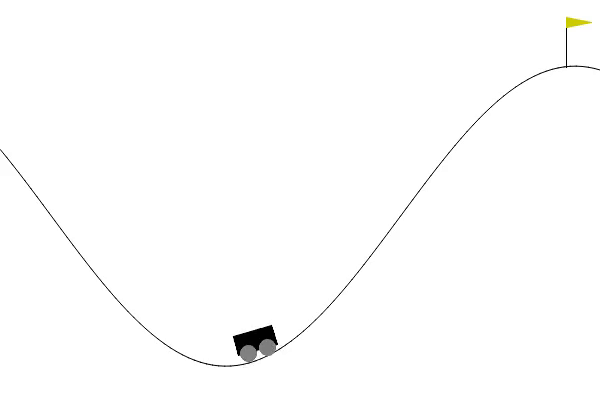
\includegraphics[height=4.5cm]{figures/images/mountain_car_frame.png}}
    \caption{Mountain Car}
  \end{subfigure}
  \hfill
  \begin{subfigure}{0.45\linewidth}
    {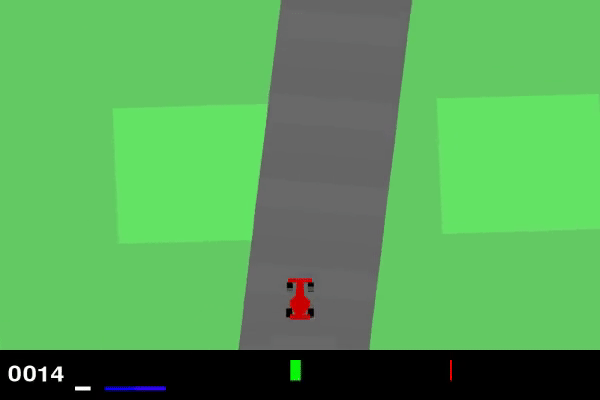
\includegraphics[height=4.5cm]{figures/images/car_racing_frame.png}}
    \caption{Car Racing}
  \end{subfigure}
  \caption[Frame from both environments]{Single frame from both of the chosen environments}
  \label{fig:game_frames}
\end{figure}


\newpage

\section{Report Structure}
The report is structured as follows:

\begin{itemize}
  \item \textbf{Background} -- discussing essential history and knowledge pertaining to the topics relevant to the project
  \item \textbf{Design \& Implementation} -- exploring the theory and reasoning behind implementation decisions, and outlining the development details of the code
  \item \textbf{Experimentation \& Evaluation} -- comparing and analysing the experimentation techniques and hyperparameters used, and examining the final results obtained
  \item \textbf{Conclusion} -- briefly summarizing the project, outlining its achievement and limitations, and exploring potential future research
\end{itemize}

\chapter{Background}
This chapter covers all of the necessary background information required to
gain a well-rounded picture of basic deep learning and reinforcement learning
concepts. We briefly go through the history of the field and the chosen games,
and then move onto the technical aspects of deep learning and reinforcement
learning, such as multilayer perceptrons and Markov decision processes.

\section{History of Reinforcement Learning}

In this section, we explore the history of reinforcement learning and its
current state; this knowledge is essential for understanding the design and
implementation concepts covered later in the report.

\subsection{Operant Conditioning}
The field of reinforcement learning started in the 1970s, through B. F.
Skinner's operant conditioning \cite{skinner1971operant}. In operant
conditioning, an animal learns to associate a particular behaviour with a
reward or punishment\footnote{In reinforcement learning research, refer to
  reward and punishment as positive reward and negative reward respectively}, and
learns the researcher's desired behaviour as it is trained over time;
\autoref{fig:skinner_box} shows the device used to do this for rats. In this
case, the agent is the rat, and the actions are pressing or not pressing the
lever, with the environment being the box the rat is interacting with; it
receives rewards in the form of food. This is the basis for shaping the
behaviour of an agent, a foundational concept in reinforcement learning; we
rely on this idea as the groundwork for this project.

\begin{figure}[H]
  \centering
  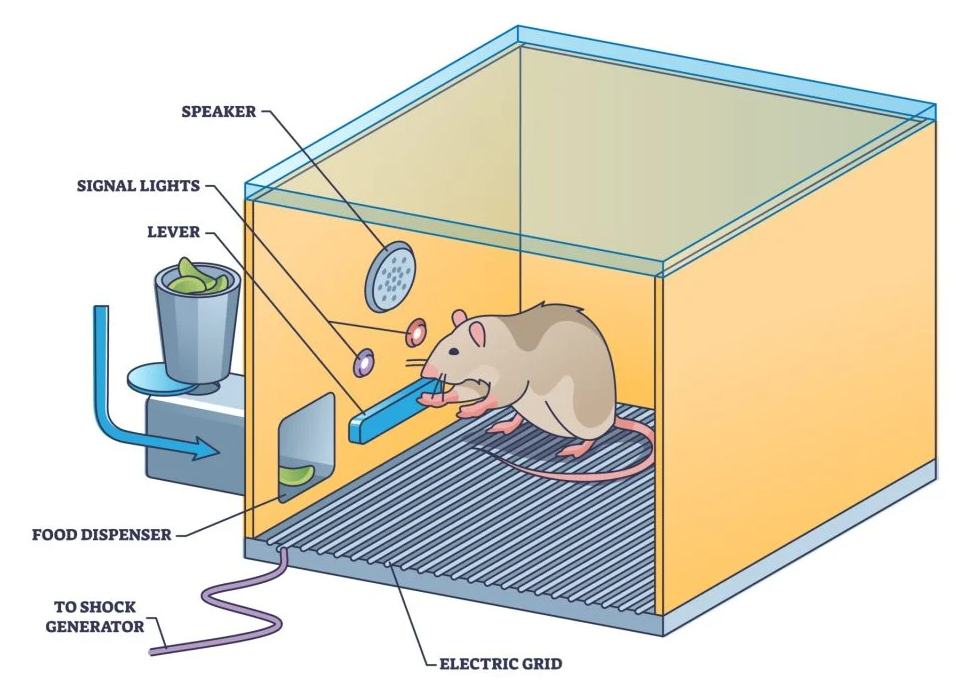
\includegraphics[width=0.5\textwidth]{figures/images/skinner_box.png}
  \caption[Skinner box]{Skinner box, used in operant conditioning experiments on rats \cite{mcleod2023b}}
  \label{fig:skinner_box}
\end{figure}


\subsection{TD Learning}
The concept of associating actions with outcomes and rewards, and
"conditioning" the agent was first applied in the context of computer science
with temporal-difference learning (TD learning), pioneered by Richard S. Sutton
in the 1980s \cite{sutton1988learning}. TD learning uses the difference between
a predicted outcome and the actual outcome of an action to update the
prediction algorithm, improving it over time. This algorithm underpins the
value based learning methods used today, including the deep Q-learning method
used in this project.

\subsection{Actor-Critic Method}
The framework for the actor-critic method was first described by Barto et al.
in 1985 as a system consisting \textit{"of a single associative search element
  (ASE) and a single adaptive critic element (ACE)"} \cite{barto1983neuronlike}.
A visual example of this method is shown in \autoref{fig:actor_critic}. This
concept lays the groundwork for the family of actor-critic methods, including
the advantage actor-critic method used in this project.

\begin{algorithm}[H]
  \caption{Tabular Actor-Critic}
  \label{alg:actor_critic}
  \begin{algorithmic}
    \State Initialize actor $\pi(a~|~s)$ with random values
    \State Initialize critic $V(s)$ with random values
    \For{episode $i$ in $1:N$}
    \State Set initial state $s_t$
    \While{$s_t$ is not terminal}
    \State Select action $a_t$ from policy $\pi(a_t~|~s_t)$ using weighted random sampling
    \State Take action $a_t$ and observe reward $r_t$ and new state $s_{t+1}$
    \State Compute TD error $\delta \gets r_t+\gamma\cdot V(s_{t+1}) - V(s_t)$
    \State Update critic values $V(s_t) \gets V(s_t) + \alpha_\text{critic}\cdot\delta$
    \State Update actor values $\pi(a_t~|~s_t) \gets \pi(a_t~|~s_t) + \alpha_\text{actor}\cdot\delta\cdot\log\pi(a_t~|~s_t)$
    \State Update state $s_t \gets s_{t+1}$
    \EndWhile
    \EndFor
  \end{algorithmic}
\end{algorithm}


\subsection{Policy Gradient Optimization}
The idea of policy gradient methods was popularized through the 1999 paper by
Sutton et al. titled "Policy Gradient Methods for Reinforcement Learning with
Function Approximation". This paper described the idea of using an
\textit{"alternative approach in which the policy is explicitly represented by
  its own function approximator"} \cite{sutton1999policy}. As the name suggests,
this method is policy based, in contrast to value based methods such as TD
learning. The idea of policy gradient optimization is what allows the actor in
the advantage actor-critic method to learn the optimal policy; we explain the
actor-critic method further in \autoref{sec:actor_critic_method_background}.

\subsection{Q-Learning}
The concept of predicting future values was later applied in the Q-learning
algorithm, proposed by Christopher Watkins in 1989 \cite{watkins1989learning}.
In Q-learning, the estimated value is the Q-value, which is the expected future
reward for each action given a state; this value is predicted using the
Q-function. An optimal policy is learned by iteratively updating this function.
A convergence proof for the algorithm was published in 1992 by Watkins and
Dayan \cite{watkins1992q}, which was generalized further in 1994 by John N.
Tsitsiklis \cite{tsitsiklis1994asynchronous}. We explore the details of
Q-learning in \autoref{sec:q_learning_background}.

\subsection{Deep Q-Learning}
Q-learning was then applied to the game of Backgammon by Tesauro et al. in
1995, producing TD Gammon \cite{tesauro1995temporal}. TD Gammon's use of neural
networks to estimate the Q-value instead of using tabular methods was a
breakthrough in reinforcement learning, as it was able to compete with and beat
expert Backgammon players. It learned complex strategies from scratch without
being explicitly programmed, which was previously unheard of.
\autoref{fig:td_gammon} shows the structure of the neural network used.

\begin{figure}[H]
  \centering
  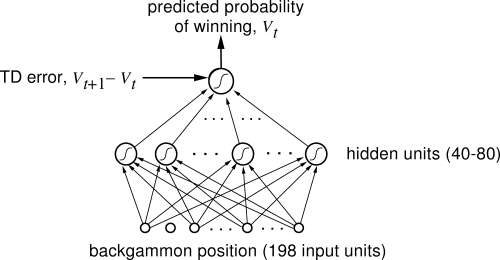
\includegraphics[width=0.7\textwidth]{figures/images/td_gammon.png}
  \caption[TD Gammon neural network]{TD Gammon neural network architecture \cite{sutton2018reinforcement}}
  \label{fig:td_gammon}
\end{figure}


Mnih et al. popularized the concept of using deep Q-networks (DQN) to play
games with their paper "Playing Atari with Deep Reinforcement Learning"
\cite{mnih2013playing}, where they achieved superhuman performance across
multiple Atari 2600 games. They later expanded the catalogue of games in 2015
\cite{mnih2015human}. We replicate the deep Q-learning strategies used in this
paper, adapting them to better suit our chosen environments.

\subsection{Asynchronous Advantage Actor-Critic}
In 2016, Mnih et al. also implemented asynchronous advantage actor-critic (A3C)
for Atari games, in their paper "Asynchronous Methods for Deep Reinforcement
Learning" \cite{mnih2016asynchronous}, vastly improving upon the performance of
the DQN. We use the concept of advantage actor-critic from this paper,
modifying it to run synchronously, as this was proven to outperform the
asynchronous version by Yuhuai Wu et al. in their 2017 paper "Scalable
trust-region method for deep reinforcement learning using Kronecker-factored
approximation" \cite{wu2017scalable}. We also make additional changes to
optimize the algorithm for Mountain Car and Car Racing.

\subsection[Recent Developments]{Recent Developments\footnote{Note the information in this section serves as context indicating the current state of the reinforcement learning space, and these concepts have not been applied directly to this project in any meaningful way}}

In 2016, a team at DeepMind developed AlphaGo to play go
\cite{silver2016mastering}, a game which was previously thought to be too
complex to be played by a program, as it has more possible board configurations
than there are atoms in the universe. AlphaGo has defeated top ranked human go
players, and, developed novel strategies after analysing expert gameplay and
using self-play to train the neural networks.

Expanding on the repertoire of games, AlphaZero was created in 2017 to master
chess, shogi and go \cite{silver2017mastering}; it achieved superhuman
performance in all three games. AlphaZero operates similarly to AlphaGo, with a
key difference being that it doesn't have access to expert gameplay; it only
uses the rule set to develop its strategies, through self-play alone.

The catalogue of games was then further expanded by MuZero in 2020, which
mastered a collection of Atari games in addition to the games played by
AlphaZero \cite{schrittwieser2020mastering}.

\begin{figure}[H]
  \centering
  \begin{subfigure}{0.26\linewidth}
    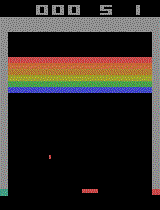
\includegraphics[height=5cm]{figures/images/breakout.png}
    \caption{Breakout}
  \end{subfigure}
  \hfill
  \begin{subfigure}{0.25\linewidth}
    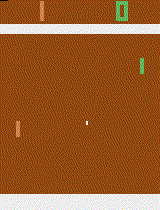
\includegraphics[height=5cm]{figures/images/pong.png}
    \caption{Pong}
  \end{subfigure}
  \hfill
  \begin{subfigure}{0.26\linewidth}
    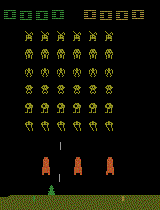
\includegraphics[height=5cm]{figures/images/space_invaders.png}
    \caption{Space Invaders}
  \end{subfigure}
  \caption[Atari games]{Popular Atari 2600 games in which AlphaZero performs with superhuman strength \cite{brockman2016gym}}
  \label{fig:atari_games}
\end{figure}


\section{Racing Games}
In this section, we briefly outline the development history of the chosen
games, and describe their mechanics as well as the reasoning for choosing these
specific games; this helps to better understand the potential improvements that
can be made to the algorithms.

Both of the racing games used in the project are well integrated into OpenAI
Gym's set of included games, alongside a larger collection of games used
commonly in reinforcement learning research \cite{brockman2016gym}.

\subsection{Mountain Car} \label{sec:mountain_car_background}
Mountain Car was first introduced by Andrew Moore in the 1990 paper "Efficient
Memory-Based Learning for Robot Control" \cite{moore1990efficient}, and was
later formalized by Satinder P. Singh and Richard S. Sutton in "Reinforcement
Learning with Replacing Eligibility Traces" \cite{singh1996reinforcement}. It
has gained popularity as a benchmark for reinforcement learning algorithms
since its introduction, and has been integrated into Gym's "Classic Control"
collection of games \cite{brockman2016gym} through which it is accessed in this
project.

The goal of Mountain Car is to reach the top of a hill, from an initial state
of the car being placed stochastically near the bottom of the hill. The car is
underpowered, meaning that an appropriate amount of force must be placed on the
car in the correct direction and from the correct position to gain momentum and
reach the yellow flag. This game has a sparse reward structure; the agent
receives a reward of -1 for each time step it takes to reach the goal, with the
episode\footnote{Episode refers to a single run of the game} ending if the
agent doesn't reach the flag within 200 time steps.

The reason for choosing Mountain Car is the simplicity of the observation and
action space; the agent receives an array containing the position and velocity
of the car, and has the option to accelerate left, do nothing or accelerate
right. This means that the game can act as a proof of concept for the
effectiveness of the chosen algorithms, and can also show the improvement
factor that domain specific enhancements provide.

\subsection{Car Racing} \label{sec:car_racing_background}
Christopher Campbell first designed Car Racing in 2014, under the name
"Top-down car" \cite{campbell2014car}. The game implements a rudimentary
physics engine to ensure the car doesn't move laterally; it contains features
such as varying surfaces that impact the car's mechanics and the ability to
drift the car, which greatly increases the difficulty of the game. Oleg Klimov
integrated the game into Gym's "Box2D" library of games \cite{brockman2016gym},
which is used by this project to access this game.

The goal of Car Racing is to complete one lap of a randomly generated track as
fast as possible, within a limited time frame. The agent is awarded -0.1 every
frame\footnote{Frame refers to a single step in the environment} and +1000/N
for every track tile visited, where N is the total number of tiles. The episode
ends if the agent doesn't complete the track within 1000 time steps or goes
outside the allowed playfield \cite{brockman2016gym}.

Contrary to Mountain Car, the reason for choosing Car Racing is the complexity
of the observation space; the agent receives a $96\times 96$ RGB image, and has
the option to do nothing, steer left, steer right, accelerate, or brake. This
combined with the complex game mechanics poses a greater challenge than
Mountain Car, and allows us to analyse the strengths and weaknesses of both
algorithms in difficult environments.

\section{Deep Learning}

Deep learning is a subset of machine learning which focuses on training
artificial neural networks on high dimensional input; this property becomes
essential in complex environments. This section discusses the techniques used
to implement the algorithms detailed in \autoref{chp:design_implementation}.

\subsection{Multilayer Perceptron}

Multilayer perceptrons (MLPs) are the foundation of artificial neural networks.
They are designed to model the neural connections in the brain, an idea first
proposed by Rosenblatt in "The Perceptron" \cite{rosenblatt1958perceptron}.

Fundamentally, an MLP is a directed graph of nodes loosely representing neurons
in the brain, which are connected to form layers. The minimum requirements for
an MLP are an input layer, at least one hidden layer, and an output layer.
These layers must be fully connected, meaning every node in one layer must be
connected to every node in the next layer. We can see an example of a simple
three layer MLP in \autoref{fig:mlp}, with two inputs, one hidden later with
three nodes, and a single output.

\begin{figure}[H]
  \centering
  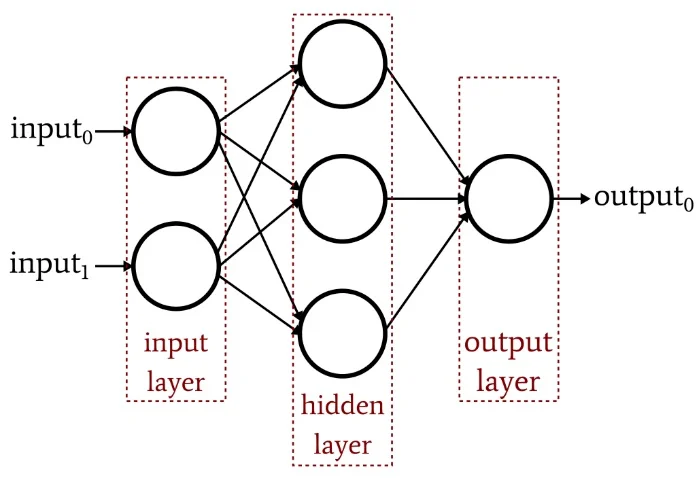
\includegraphics[width=0.5\textwidth]{figures/images/mlp.png}
  \caption[Multilayer perceptron]{Simple multilayer perceptron \cite{ledell2021statistical}}
  \label{fig:mlp}
\end{figure}


Each neuron takes the inputs $\bigl[ \begin{smallmatrix}
      x_1 \\
      \hdots \\
      x_n
    \end{smallmatrix}\bigr]$,
and computes the dot product with its stored weights
$\bigl[ \begin{smallmatrix}
      w_1 \\
      \hdots \\
      w_n
    \end{smallmatrix}\bigr]$. A bias term, $b$, is added to the result, and finally, an activation function $\phi(x)$ is applied to produce the node's output. A schematic representation of this is shown in \autoref{fig:neuron}. Different activation functions and the reasons for choosing them are explored further in \autoref{sec:activation_functions}.

\begin{gather*}
  x_{out} = \phi\left(
  \begin{bmatrix}
      x_1    \\
      \hdots \\
      x_n
    \end{bmatrix}
  \cdot
  \begin{bmatrix}
      w_1    \\
      \hdots \\
      w_n
    \end{bmatrix}
  + b\right)
\end{gather*}

\begin{figure}[H]
  \centering
  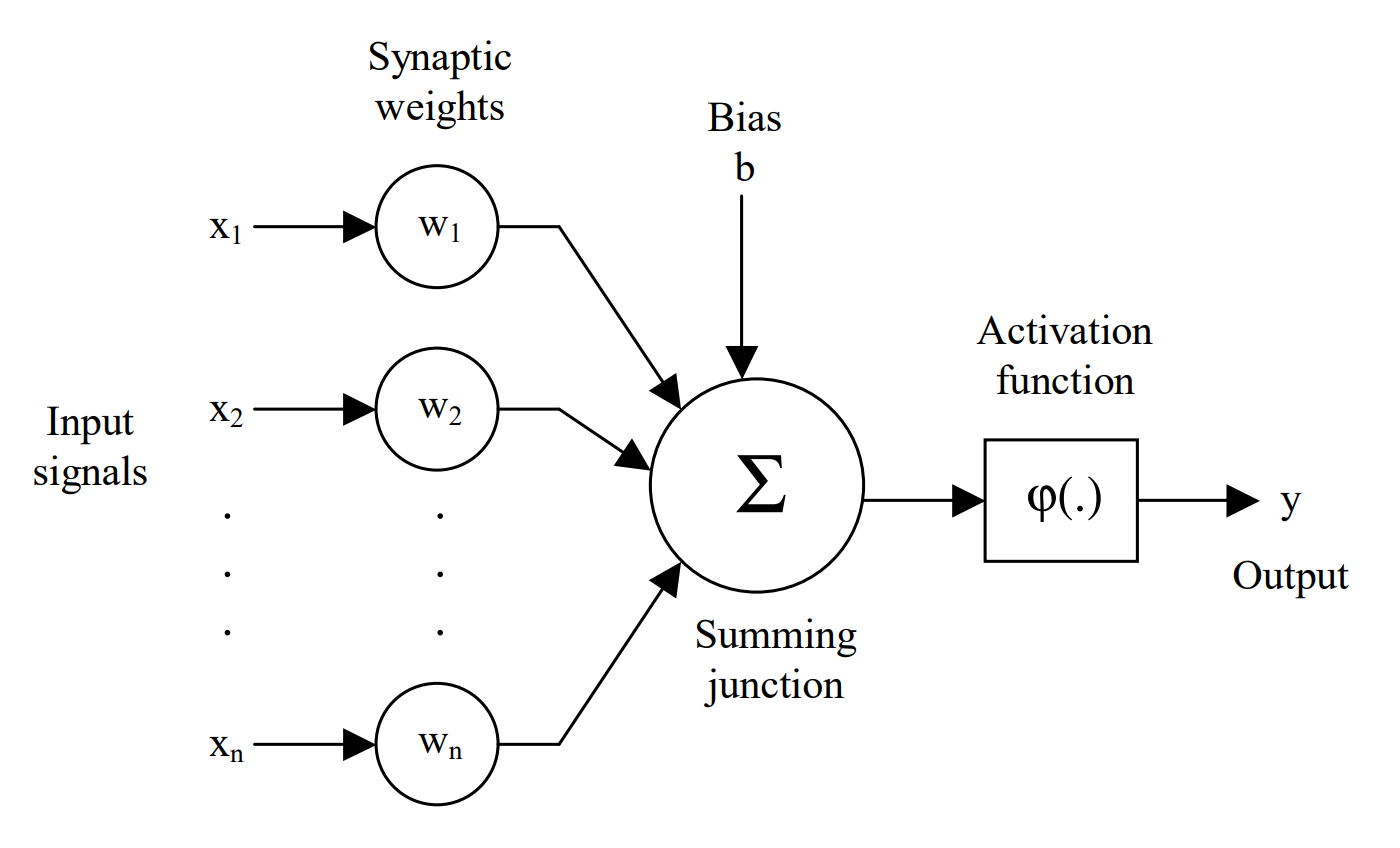
\includegraphics[width=0.7\textwidth]{figures/images/neuron.png}
  \caption[Single neuron]{Data flow and operations through single neuron \cite{csaji2001approximation}}
  \label{fig:neuron}
\end{figure}


A forward pass through the neural network is conducted layer by layer, with the
output of one layer becoming the input to the nodes in the next layer. The
final output of the MLP is the output of the last layer, which could represent
action probabilities, value estimations, etc.

Training the MLP means optimizing the weights and biases to maximize the
reward, which is done using backpropagation. This involves computing the
gradient of the reward function with respect to the weights, and using a
gradient descent method to update them, in order to reduce the difference
between the predicted output and actual output and thus improve the neural
network's prediction capabilities.

\subsubsection{Fully Connected Layers} \label{sec:connected_layers}

Due to the requirement of fully connected layers\footnote{We also refer to
  fully connected layers as "dense" layers, as this project uses Keras to
  implement the neural networks; all of the concepts are transferrable to any
  other framework}, these networks are prone to overfitting\footnote{Overfitting
  occurs when a model gives accurate predictions for the training data, but
  inaccurate predictions for unseen data} to the input and are therefore less
generalizable to novel inputs. Techniques to mitigate this issue include:

\begin{itemize}
  \item \textbf{Regularization} -- adding a penalty term (usually proportional to the weights) to the loss function, forcing the network to have sparse weights \cite{krogh1991simple}
  \item \textbf{Dropout} -- randomly "removing" neurons during training, preventing the network from relying too heavily on any one neuron \cite{srivastava2014dropout}
  \item \textbf{Batch normalization} -- normalizing the input of each layer to the neural network to have zero mean and unitary standard deviation, improving training stability and speed \cite{ioffe2015batch}
\end{itemize}

\subsubsection{Activation Functions} \label{sec:activation_functions}

The primary reason for using activation functions in MLPs is to introduce
non-linearity into the network \cite{sharma2017activation}. Without using them,
the output of a neural network can be described as a linear combination of the
input vector; activation functions allow us to model the complex non-linear
relationships between the network's inputs and outputs. Additionally,
activation functions help to introduce sparsity into the neural network, by
setting some neuron activations to zero; this can be useful in reducing
overfitting and improving the network's generalization.

Every activation function has its strengths and weaknesses. Commonly used
activation functions include:

\begin{itemize}
  \item \textbf{Rectified linear unit (ReLU)} -- returns 0 for any negative input and the input value for any positive input; often used in between convolution layers in convolutional neural networks
        $$\text{ReLU}(x) = \max(0,~x)$$
  \item \textbf{Softmax} -- maps input values to a probability distribution over the output classes, ensuring that the sum of the probabilities is equal to 1; often used in the output layer of neural networks that produce probability values
        $$\sigma(\vec{z})_i = \frac{e^{z_i}}{\sum_{j=1}^K e^{z_j}}$$
  \item \textbf{Tanh} --  maps inputs to a value between -1 and 1; often used in the fully connected hidden layers of a neural network as it can produce both positive and negative values
        $$\tanh(x) = \frac{e^x - e^{-x}}{e^x + e^{-x}}$$
\end{itemize}

We can see the graphical representation of these functions in
\autoref{fig:activation_functions}.

\begin{figure}[H]
  \centering
  \begin{subfigure}{0.27\linewidth}
    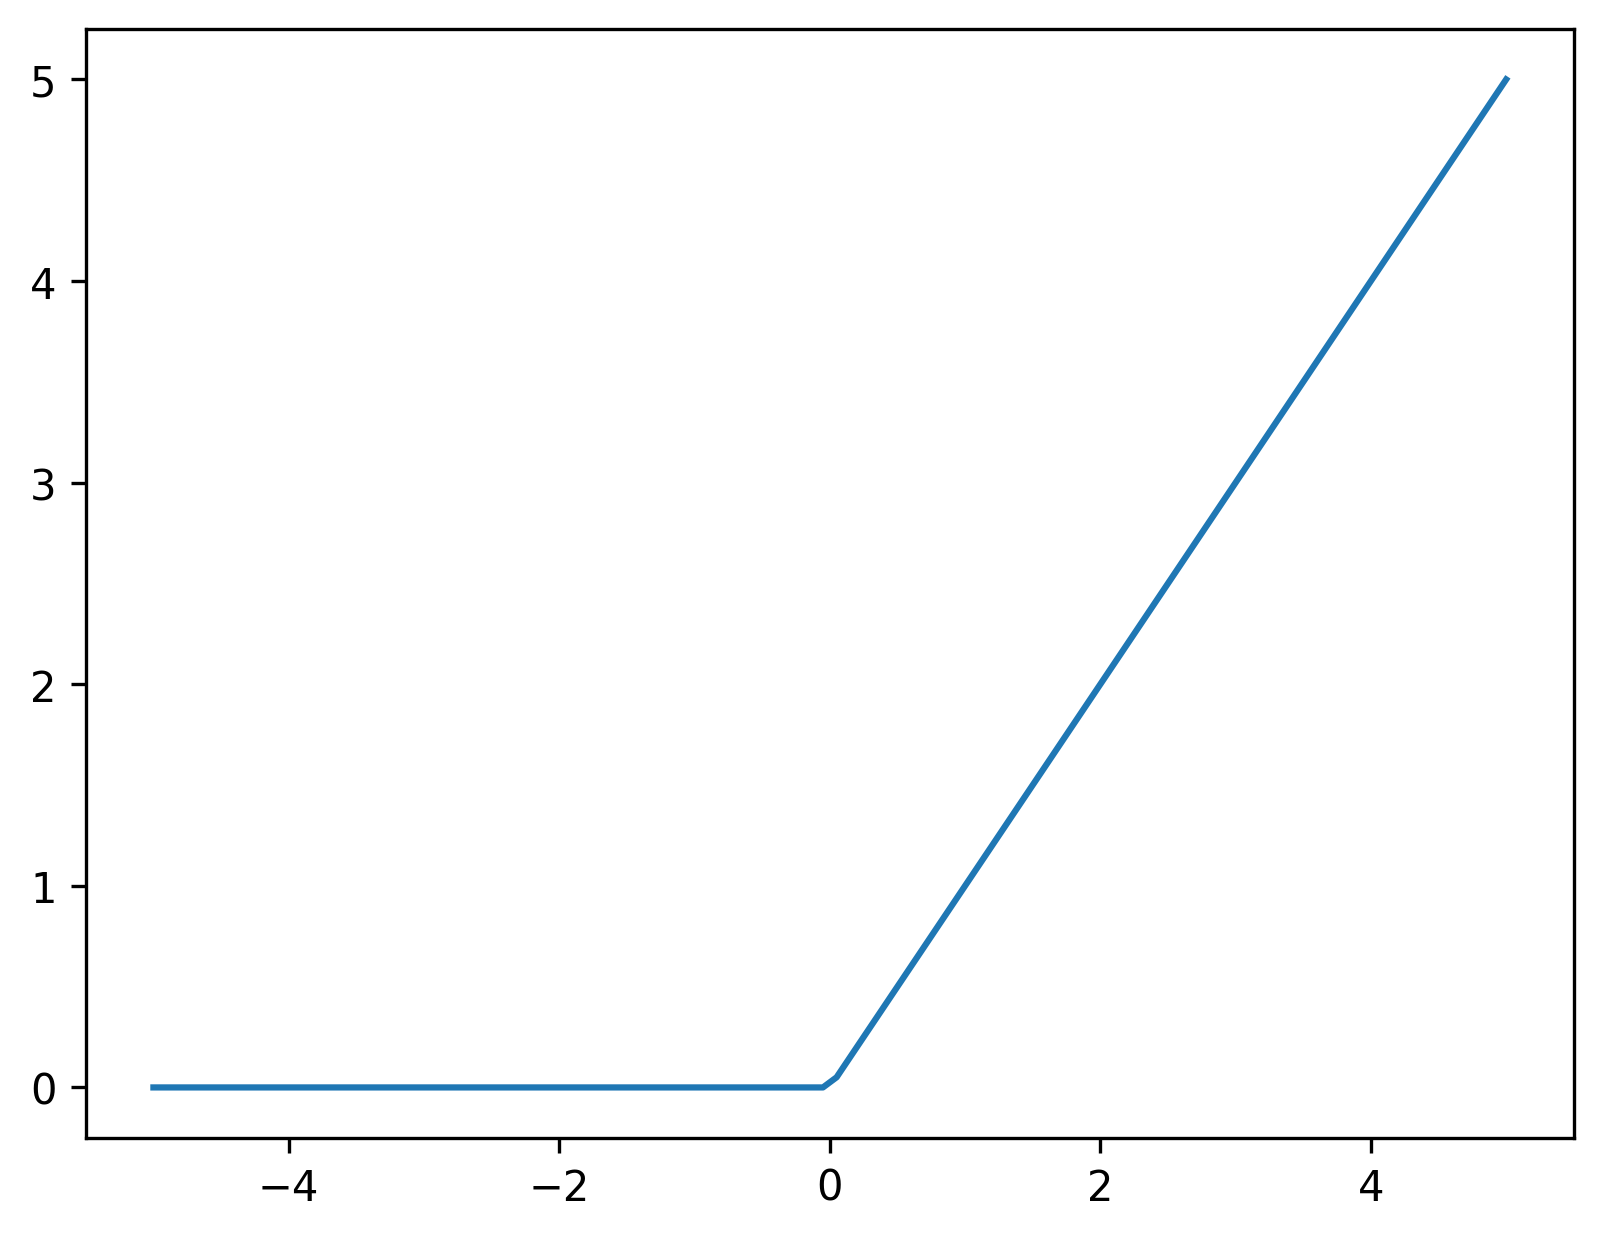
\includegraphics[height=3cm]{figures/images/relu.png}
    \caption{ReLU}
  \end{subfigure}
  \hfill
  \begin{subfigure}{0.28\linewidth}
    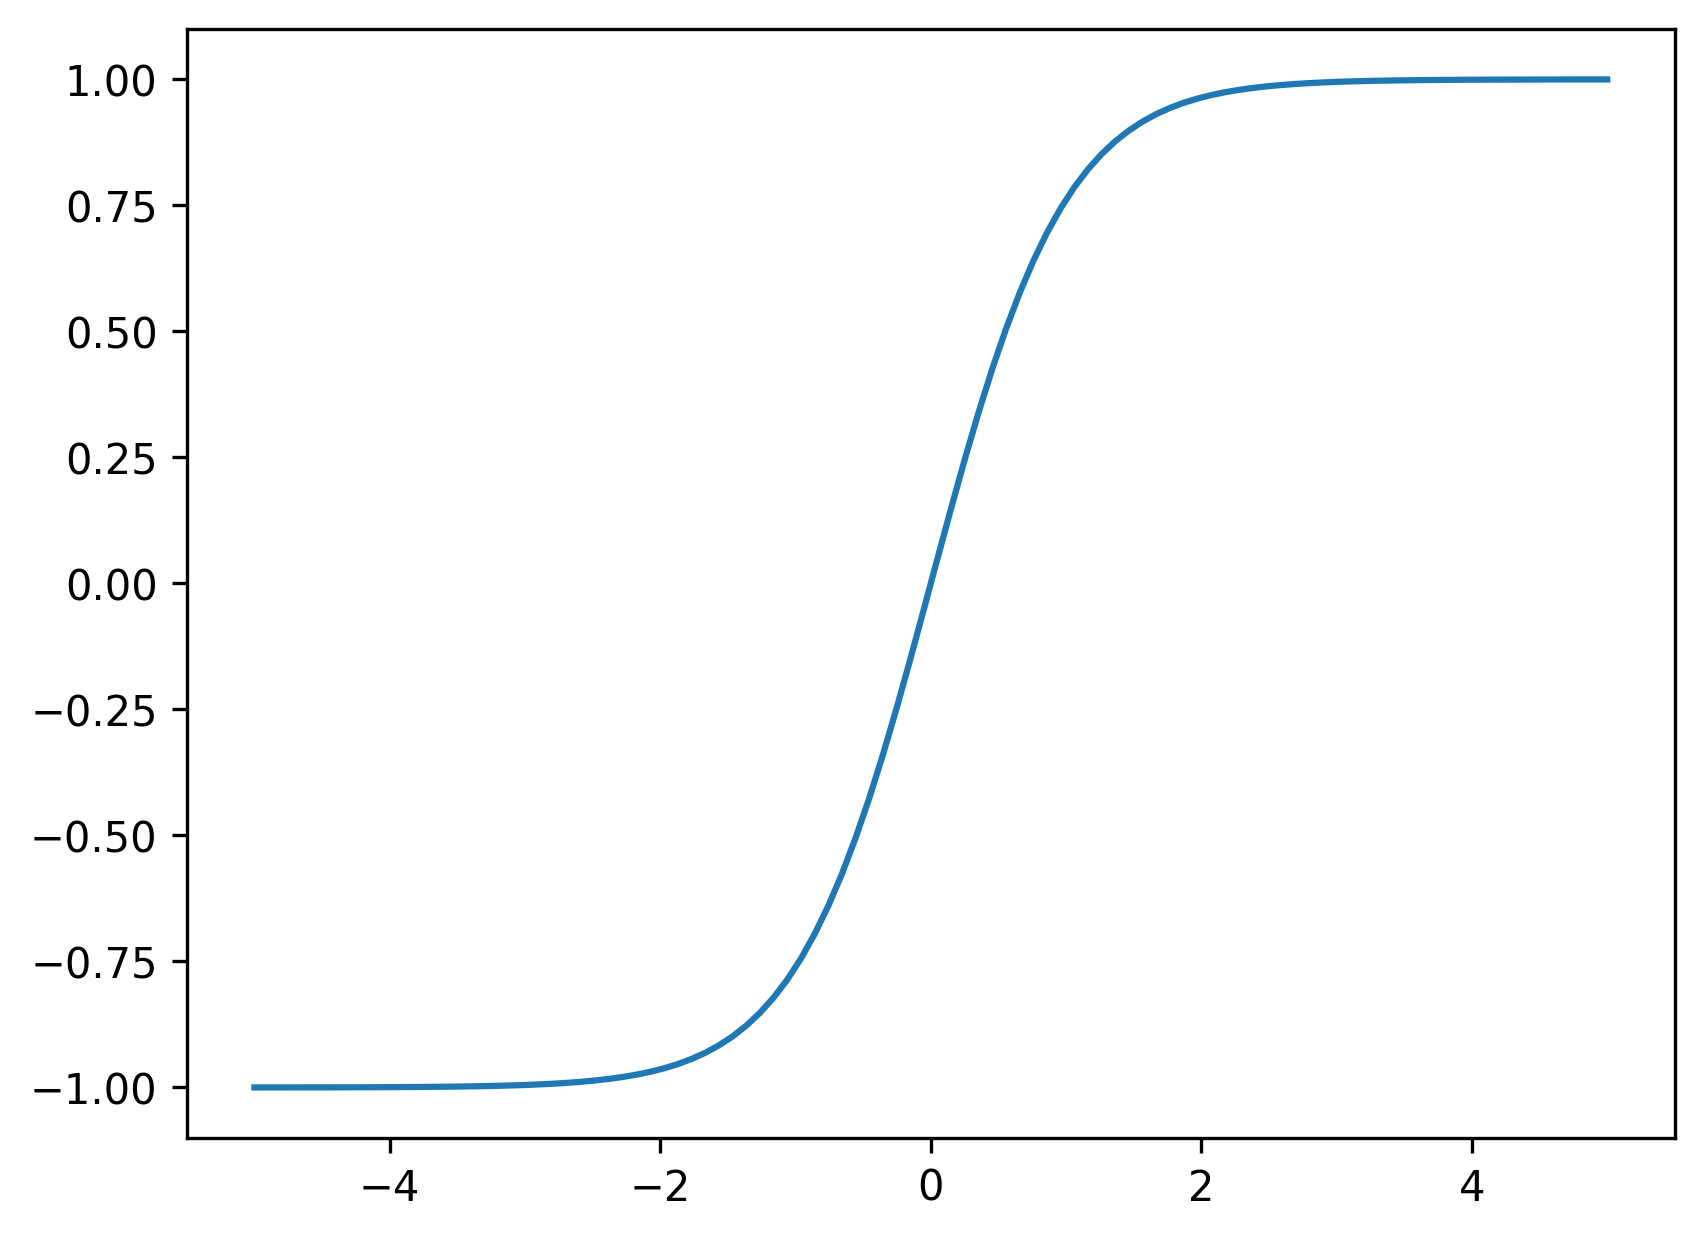
\includegraphics[height=3cm]{figures/images/tanh.png}
    \caption{Tanh}
  \end{subfigure}
  \hfill
  \begin{subfigure}{0.28\linewidth}
    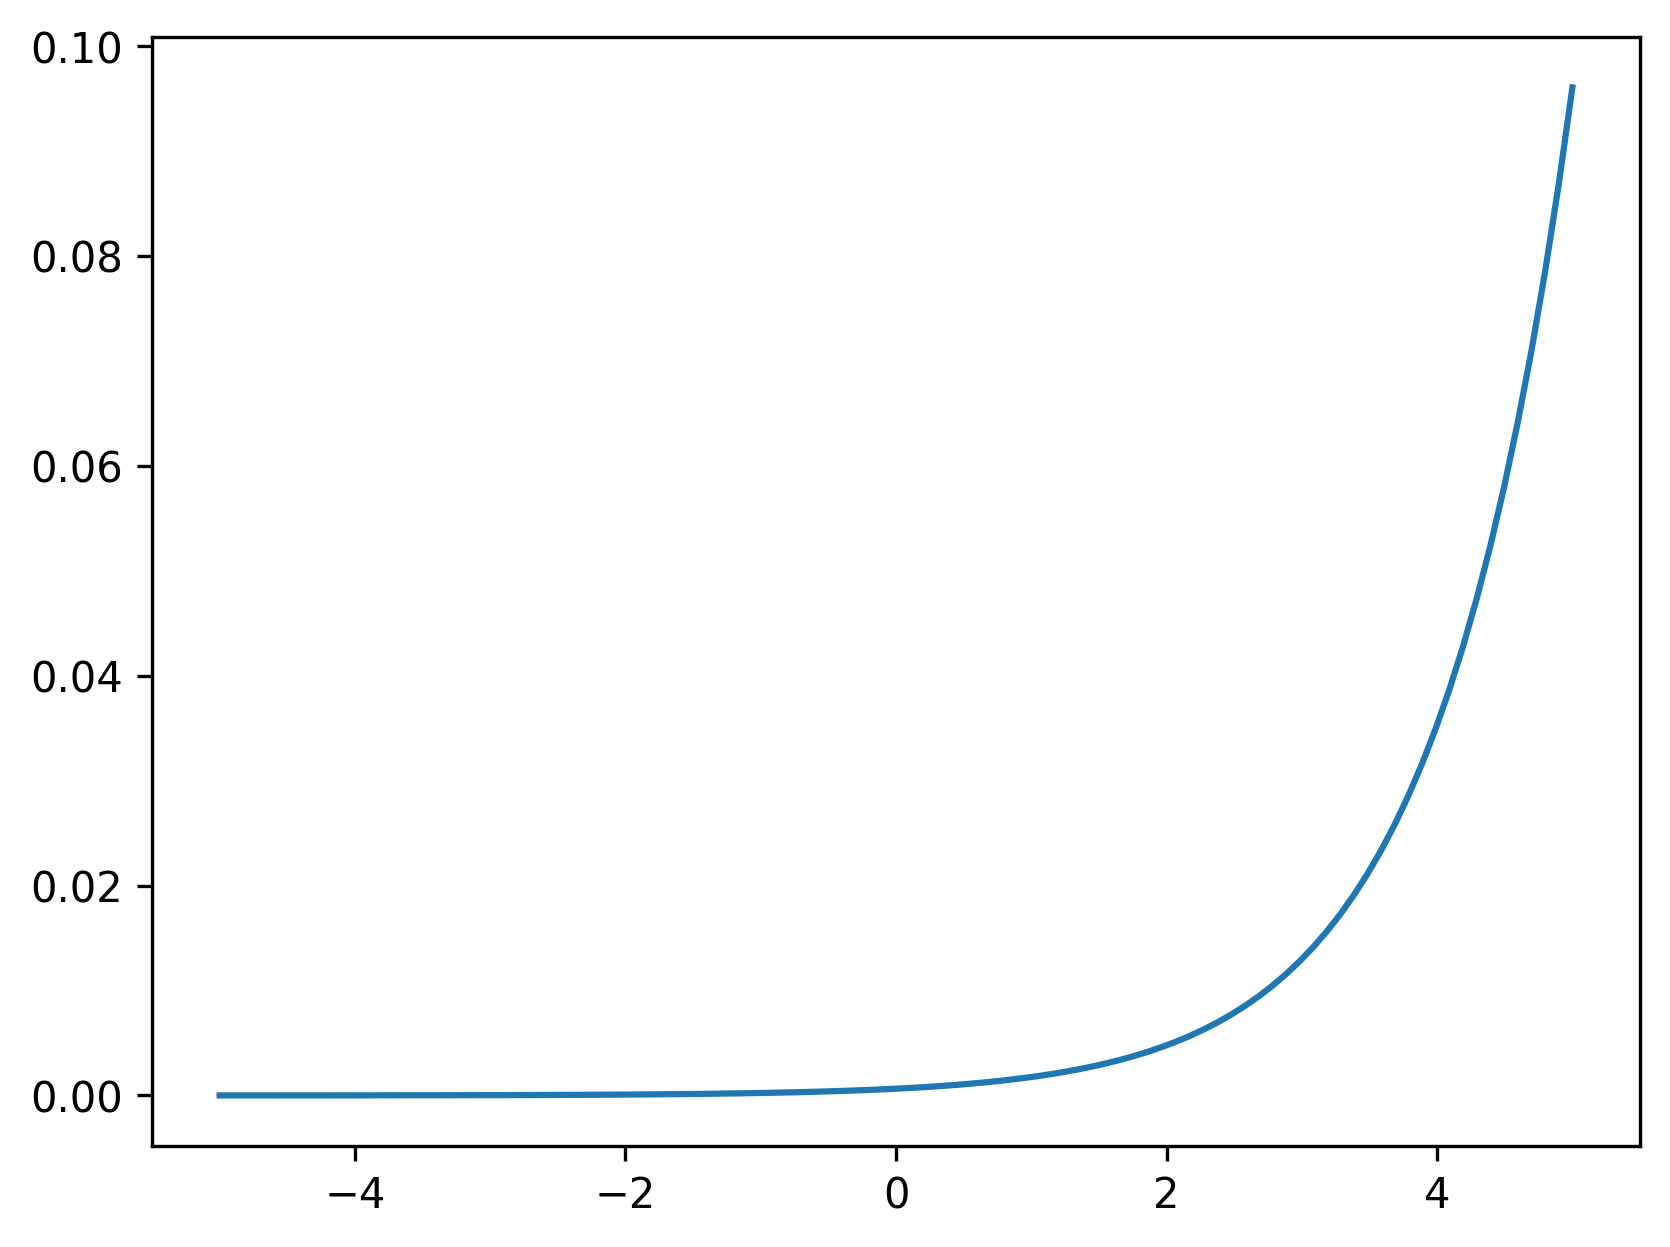
\includegraphics[height=3cm]{figures/images/softmax.png}
    \caption{Softmax}
  \end{subfigure}
  \caption[Activation functions]{Commonly used activation functions}
  \label{fig:activation_functions}
\end{figure}


\subsection{Convolutional Neural Network}

While it is possible to acquire vectorized data about the direct properties of
the environment and agent (for example, car position and velocity in Mountain
Car), this is not always the case. We often only have access to observational
image data (such as the bird's eye view in Car Racing), and we need to make
decisions based on this limited subset of information. Due to the
multidimensional nature of images, we need to extend the functionality of our
neural networks to support these types of inputs; convolutional neural networks
(CNN) provide a way for us to do this\footnote{The functionality provided by
  CNNs can technically be implemented using MLPs, though it is much more
  difficult}. These networks maintain the spatial structure of the input image
data, and can take better advantage of localized features by using
convolutional filters and pooling layers, explained further below.

\subsubsection{Filters}

The cornerstone of CNNs is the convolutional filter. It is an $n\times n$ grid
of values; the dot product is computed between the filter weights and the input
values, as shown in \autoref{fig:conv}.

\begin{figure}[H]
  \centering
  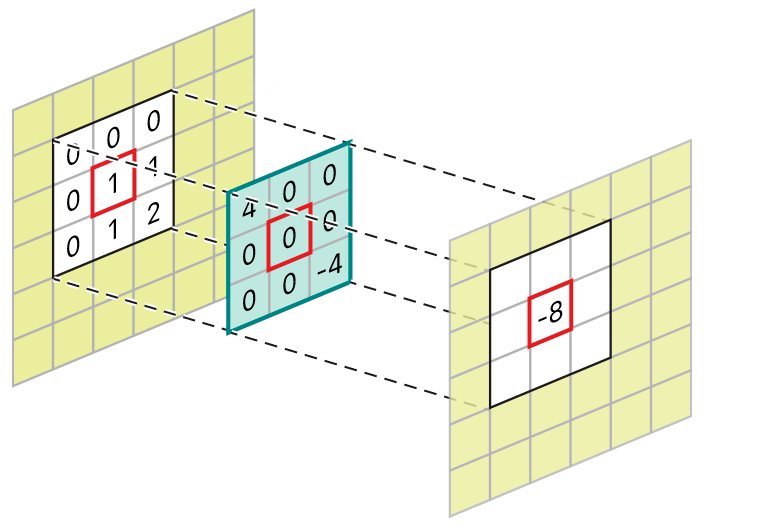
\includegraphics[width=0.5\textwidth]{figures/images/conv.png}
  \caption[Convolution filter]{Convolution filter of size $3\times 3$ being applied to an image \cite{apple0000blurring}}
  \label{fig:conv}
\end{figure}


These filters scan the input, similar to a sliding window. The step size of the
window is determined by its stride $s$, which denotes how many values to move
the filter by at each step during the convolution operation.

For each convolutional layer in a CNN, we usually have multiple filters, the
result of which is a separate layer for the output of each of the filters, as
shown in \autoref{fig:cnn}.

The weights of the filters are learnable; they are analogous to the node
connection weights in MLPs, and are optimized through gradient descent
algorithms.

\begin{figure}[H]
  \centering
  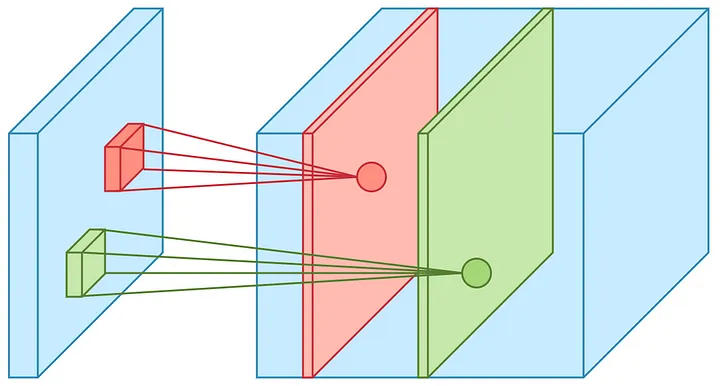
\includegraphics[width=0.5\textwidth]{figures/images/cnn.png}
  \caption[Convolutional neural network output]{Result of convolutional neural network with multiple filters applied to an input \cite{dertat2017applied}}
  \label{fig:cnn}
\end{figure}


\subsubsection{Layer Types}

The most common types of layers used in CNNs and their roles in the network are
described below:

\begin{itemize}
  \item \textbf{Convolution} -- uses a set of learnable filters to extract features and create a feature map, from either the input image or intermediary convolutional layers \cite{o2015introduction}
  \item \textbf{Pooling} -- downsamples the feature maps produced by the convolutional layers; reduces the spatial dimensions of the feature map while retaining the important information, for example max pooling, which involves taking the maximum values within specific regions of the feature map \cite{lecun2015deep}
  \item \textbf{Activation} -- applies a non-linear activation function to the output of the convolutional and pooling layers, usually ReLU
  \item \textbf{Flattening} -- converts the multidimensional output of convolutional, pooling, and activation layers into a 1D vector that can be processed by a dense layer
  \item \textbf{Dense} -- connects the output of the convolutional and pooling layers to the output layer of the network; the same as the fully connected layers in MLPs
\end{itemize}

We can see an example of the VGG16 CNN architecture in \autoref{fig:cnn_vgg},
which uses multiple sets of convolutional layers with ReLU activation and max
pooling layers, followed in the end by a series of fully connected layers. This
type of architecture is commonly used across the field of computer vision and
pattern recognition research \cite{simonyan2014very, lecun2015deep}.

\begin{figure}[H]
  \centering
  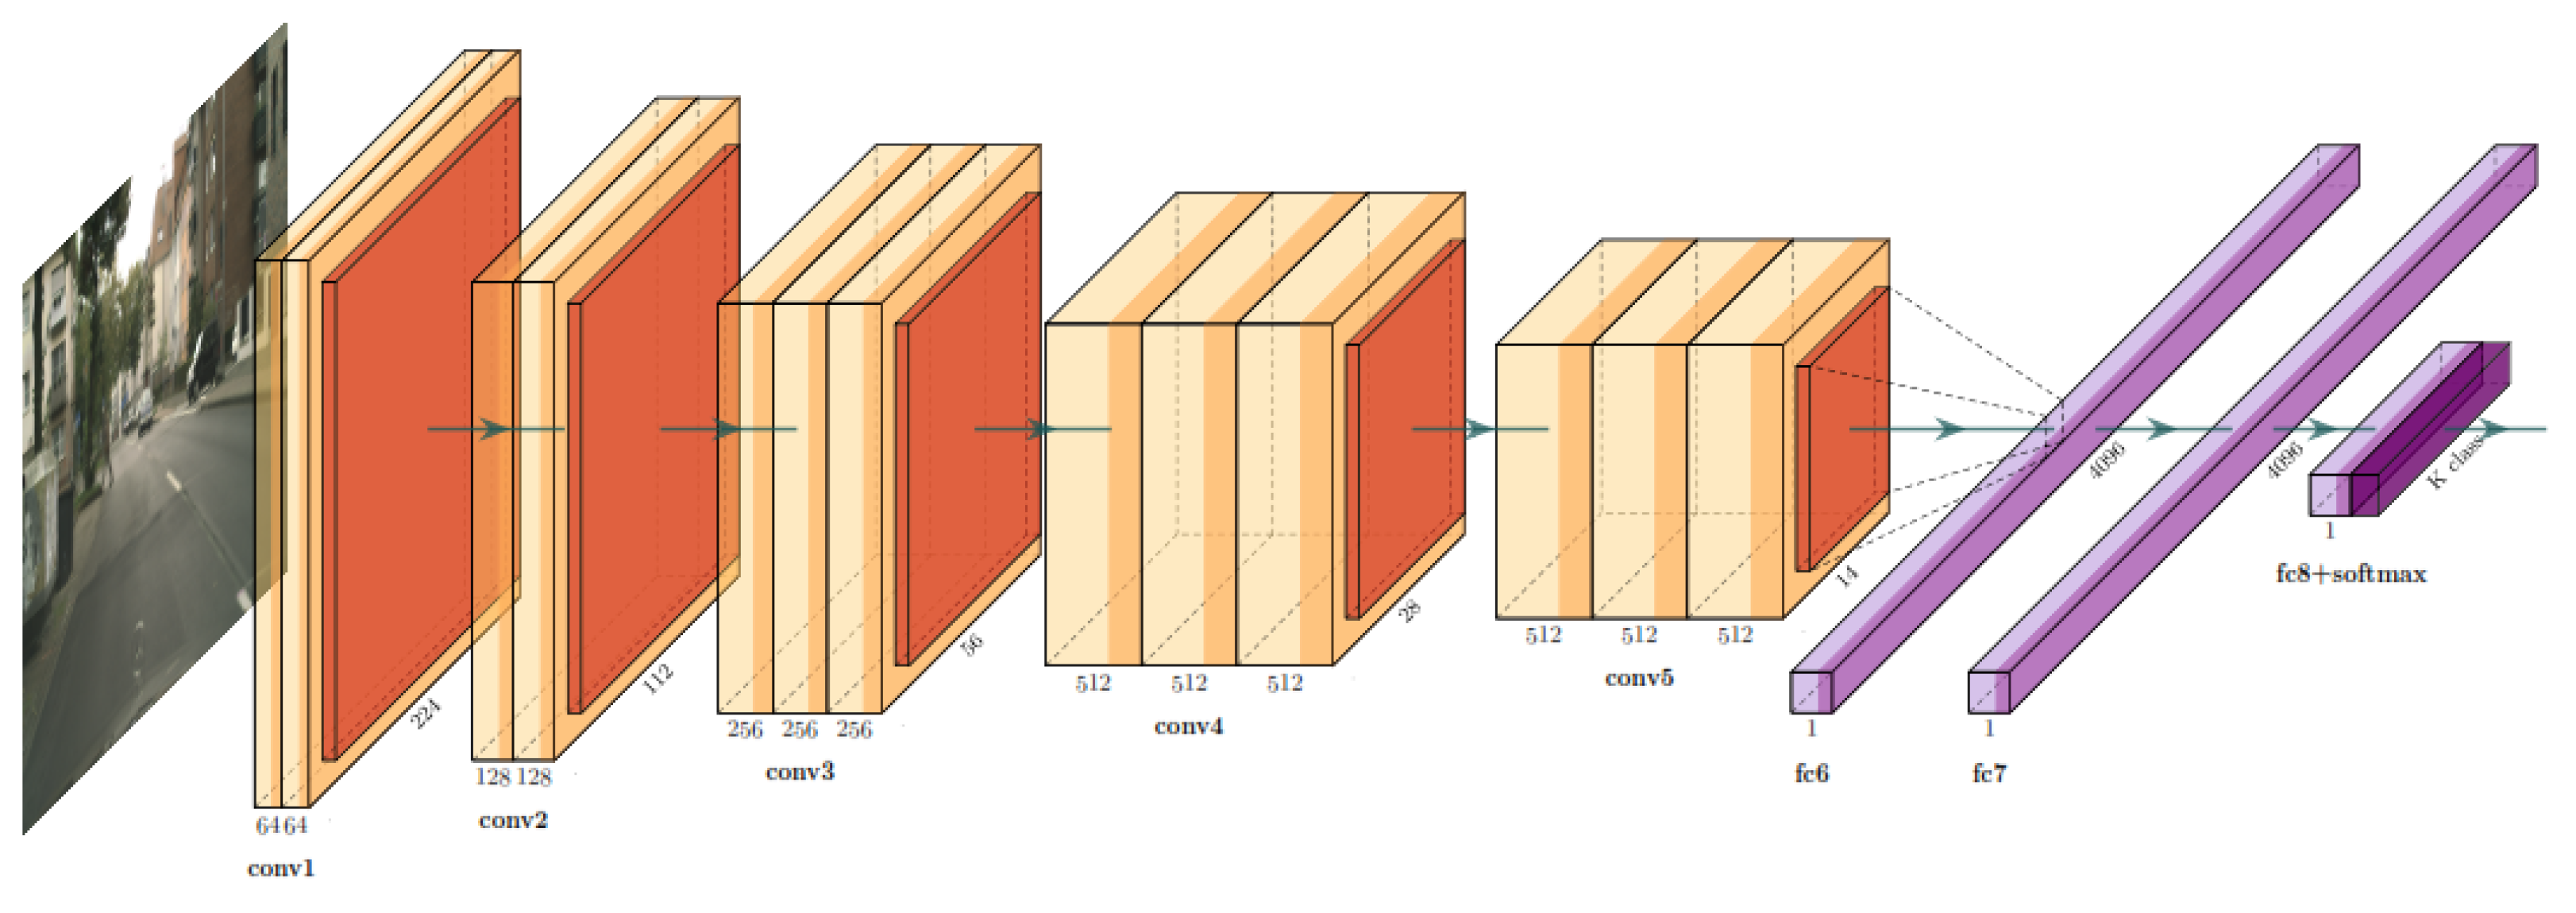
\includegraphics[width=0.9\textwidth]{figures/images/cnn_vgg.png}
  \caption[VGG16 CNN architecture]{VGG16 CNN architecture \cite{cardenas2022complex}}
  \label{fig:cnn_vgg}
\end{figure}


\newpage

\section{Reinforcement Learning} \label{sec:reinforcement_learning}

Reinforcement learning (RL) is an area of machine learning that focuses on
teaching agents to make decisions in environments, by rewarding desired
behaviours and punishing undesired ones. The goal of RL is to find the set of
actions to take in each state to maximize the cumulative reward over time,
called the policy. \autoref{fig:rl} shows the data flow through the various
components of reinforcement learning methods.

\begin{figure}[H]
  \centering
  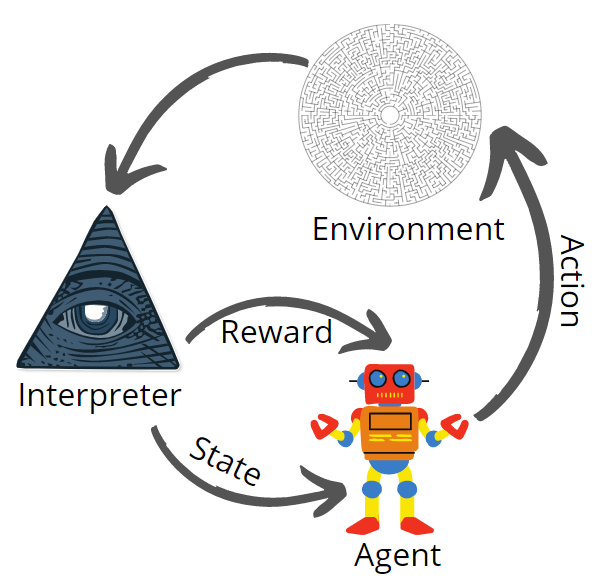
\includegraphics[width=0.4\textwidth]{figures/images/rl.png}
  \caption[Reinforcement learning flow]{Components and data flow of reinforcement learning, showing the interaction between the agent and environment; the agent takes an action based on the current state, receives a new state and a reward, and incrementally improves \cite{erainnovator2021reinforcement}}
  \label{fig:rl}
\end{figure}


The focus of this project is model-free algorithms, which means that the agent
is able to learn through trial and error by receiving and processing rewards,
without any external input. Unlike model-based algorithms, it does not rely on
an explicit model of the environment's dynamics or the reward function. The
details of model-based algorithms are not covered in this report.

\subsection{Markov Decision Process}

Markov decision processes (MDPs) are a formalization of the problem of learning
an optimal policy for an agent to take actions in an environment. The following
definitions pertaining to Markov decision processes are adapted from David
Silver's lecture series on Reinforcement Learning \cite{silver2015lecture}.

\begin{definition}
  A \textit{Markov decision process} is a tuple $\langle\mathcal{S}, \mathcal{A}, \mathcal{P}, \mathcal{R}, \gamma\rangle$
  \begin{itemize}[label={}]
    \item $\mathcal{S}$, finite set of states
    \item $\mathcal{A}$, finite set of actions
    \item $\mathcal{P}$, state transition probability matrix
          \begin{itemize}[label={}]
            \item $\mathcal{P}_{ss'}^a = \mathbb{P}~[S_{t+1}=s'\mid S_t=s,~A_t=a]$
          \end{itemize}
    \item $\mathcal{R}$, reward function
          \begin{itemize}[label={}]
            \item $\mathcal{R}_{s}^a = \mathbb{E}~[R_{t+1}\mid S_t=s,~A_t=a]$
          \end{itemize}
    \item $\gamma$, discount factor
          \begin{itemize}[label={}]
            \item $\gamma\in[0,1]$
          \end{itemize}
  \end{itemize}
\end{definition}

The state transition probability matrix $\mathcal{P}$ defines the probability
of moving from one state to another state when the agent takes a specific
action. The reward function $\mathcal{R}$ defines the immediate reward
(positive or negative) the agent receives for taking a particular action in any
given state. The discount factor $\gamma$ determines how much the system values
future rewards; $\gamma = 1$ means that future rewards are valued equally to
immediate rewards, while $\gamma = 0$ means only the immediate reward is
valued. The discount factor is a hyperparameter optimized during training, with
common values being $\gamma\in[0.95,0.99]$.

\begin{definition}
  A \textit{policy} $\pi$ is a distribution over actions given states
  $$\pi(a\mid s)=\mathbb{P}~[A_t=a\mid S_t=s]$$
\end{definition}

The policy $\pi$ is a decision-making strategy, used by the agent to determine
which action to take. It can either be a stochastic function that provides the
agent with a probability distribution over the set of possible actions for the
given state, or a deterministic function, meaning it maps the given state to a
specific action. A key feature of MDPs is that the agent's behaviour depends
only on the current state, excluding all previous states. The implications of
this are discussed in \autoref{sec:markov_property}.

\begin{definition}
  The \textit{return} $G_{t}$ is the total discounted reward from time-step $t$
  $$G_{t}=R_{t+1}+\gamma\cdot R_{t+2}+\ldots=\sum_{k=0}^{\infty}\gamma^{~k}\cdot R_{t+k+1}$$
\end{definition}

\begin{definition} \label{def:state_value_function}
  The \textit{state-value function} $v_\pi(s)$ of an MDP is the expected return starting from state $s$, and then following policy $\pi$
  $$v_\pi(s)=\mathbb{E}_{\pi}~[G_{t}\mid S_{t}= s]$$
\end{definition}

\begin{definition} \label{def:action_value_function}
  The \textit{action-value function} $q_\pi(s,~a)$ of an MDP is the expected return starting from state $s$, taking action $a$, and then following policy $\pi$
  $$q_\pi(s,~a)=\mathbb{E}_{\pi}~[G_{t}\mid S_{t}= s,~A_{t}= a]$$
\end{definition}

\begin{definition}
  The \textit{optimal state-value function} is the maximum value function over all policies
  $$v_*(s)=\max_\pi v_\pi(s)$$
\end{definition}

\begin{definition}
  The \textit{optimal action-value function} is the maximum action-value function over all policies
  $$q_*(s,~a)=\max_\pi q_\pi(s,~a)$$
\end{definition}

The goal of an MDP is to find the optimal action-value function, by finding a
policy $\pi$ that maximizes the return $G_{t}$. Once this is found, the MDP can
be considered solved, as we know which actions in any given state lead to the
highest reward.

\subsubsection{Markov Property} \label{sec:markov_property}

Simply put, the Markov property can be described as follows: the future state
of the system is independent of its past history, given its current state
\cite{markov1954theory}. We formalize this in the definition below.

\begin{definition}
  The \textit{Markov property} is a property of Markov (decision) processes
  $$\mathbb{P}~[S_{t+1}=s~|~S_t,~S_{t-1},\ldots, S_1] = \mathbb{P}~[S_{t+1}=s~|~S_t]$$
\end{definition}

This property is also known as memorylessness, because the system has no
recollection of any past states. However, this also raises the issue where the
network might not have enough information to make a decision. For example, in
\autoref{fig:car_racing_frame}, the speed of the car can not be deduced from a
single frame.

\begin{figure}[H]
  \centering
  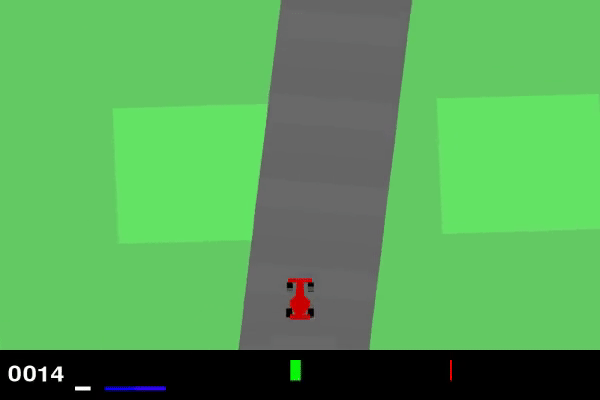
\includegraphics[width=0.5\textwidth]{figures/images/car_racing_frame.png}
  \caption[Car Racing frame]{Single frame from the Car Racing environment}
  \label{fig:car_racing_frame}
\end{figure}


To solve this, a frame stack can be used; the frame stack stores a rolling
history of states, which is then passed to the network instead of just a single
frame\footnote{A frame stack was not required for Mountain Car as the agent
  receives exact information about the car's speed and position}. This provides
the network with sufficient information to predict the optimal action. The size
of the frame stack is another hyperparameter to be optimized during training.

\subsection{Policy-Based vs Value-Based}

There are two prominent approaches to solving RL problems: policy-based
methods, and value-based methods. Hybrid methods, such as actor-critic,
incorporate components from both methods.

Policy-based methods, such as proximal policy optimization
\cite{schulman2017proximal}, focus on directly learning the policy that the
agent should follow to maximize the cumulative reward. These methods optimize
the policy using gradient descent, where the objective is to maximize the
return $G_t$. They are highly effective in continuous action space
environments, but suffer from high variance in the policy updates, leading to
learning instability.

Value-based methods, such as (deep) Q-learning, instead focus on learning the
value function, which estimates the expected cumulative reward from a given
state or state-action pair. The goal is to find the optimal state-value or
action-value function, which can be used to derive an optimal policy. Value
based methods have much more stable learning, however, they can only learn
deterministic policies.

\subsection{On-Policy vs Off-Policy} \label{sec:on_vs_off_policy}

The difference between on-policy and off-policy algorithms is whether the
behaviour policy\footnote{Behaviour policy refers to the policy used to
  determine the action to be taken in the environment} is the same as the target
policy\footnote{Target policy refers to the policy that is being "trained" in
  the neural network, which is the one we would like to optimize}. A2C is an
example of an on-policy algorithm, while DQNs are off-policy algorithms.

In an on-policy algorithm, the agent updates its target policy only using
experience generated by the same target policy. The benefit of on-policy
algorithms is that they provide more stable learning compared to off-policy
algorithms, since the same policy is used throughout the whole process.
However, it can also be less sample-efficient\footnote{Sample efficiency is the
  capability of an agent to learn with few samples}, as the collected data can
only be used once: to update the current policy.

An off-policy algorithm updates its target policy using experience generated by
a different behaviour policy. The advantage of this is that the agent can reuse
past experiences for faster learning through techniques like experience replay,
explored further in \autoref{sec:experience_replay}. However, it can also be
more challenging to stabilize the learning process, as the target policy can be
misaligned with the behaviour policy, making it a moving target.

\subsection{Exploration vs Exploitation}

The exploration-exploitation trade-off is a critical concept in RL. It
determines how the agent balances the need for exploiting the current knowledge
to maximize the reward with the need for deviating from the policy and
gathering new information for a potentially higher reward.

Too much exploration can lead to suboptimal policies and inefficient learning,
while too little exploration can lead to a lack of diversity in actions and a
failure to discover better policies. In this project, we used the
$\epsilon$-greedy approach for the DQN, and entropy regularization for the A2C
algorithm; we discuss the implementation details of these methods further in
\autoref{sec:epsilon_greedy} and \autoref{sec:entropy_regularization}
respectively.

These methods work extremely well: $\epsilon$-greedy has been shown to produce
scores better than humans \cite{mnih2013playing} in DQNs, and entropy
regularization with A2C also produces superhuman performance on similar tasks
\cite{mnih2016asynchronous}.

A few of the more advanced exploration methods include upper confidence bounds,
optimistic initialization, Boltzmann exploration, model-based exploration, and
Thompson sampling \cite{mcfarlane2018survey, ladosz2022exploration,
  gou2019dqn}; these have not been implemented in this project.

\subsection{Q-Learning} \label{sec:q_learning_background}

Q-learning is an instance of TD learning that focuses on learning an
action-value function \cite{watkins1989learning}; it is an algorithm that uses
a Q-table to store the expected future rewards, or the Q-values of taking each
action in a given state. An example of a Q-table for Mountain Car is shown in
\autoref{table:q}.

\begin{table}[H]
  \centering
  \begin{tabular}{|c|c|c|c|c|}
    \hline
    \multicolumn{2}{|c|}{\multirow{2}{*}}                    & \multicolumn{3}{c|}{\textbf{Action}}                                                      \\
    \cline{3-5}
    \multicolumn{2}{|c|}{\multirow{-2}{*}{\textbf{Q-table}}} & \textbf{Left (0)}                    & \textbf{Nothing (1)} & \textbf{Right (2)}          \\
    \hline
    \multirow{4}{*}{\textbf{State}}
                                                             & \bm{$S_0$}                           & -0.5                  & -0.2                & -0.8    \\
                                                             & \bm{$S_1$}                           & -0.1                  & -0.7                & -0.5   \\
                                                             & \textbf{\vdots}                      & \vdots               & \vdots             & \vdots \\
                                                             & \bm{$S_n$}                           & -1.0                 & -0.5                & -0.2    \\
    \hline
  \end{tabular}
  \caption[Q-table example]{Q-table showing hypothetical state-action pairs for Mountain Car}
  \label{table:q}
\end{table}


The algorithm starts with a randomly initialized table, and as the agent
interacts with the environment, it updates the table by estimating the expected
future reward for each state-action pair.

Below are the formal definitions of the Q-learning temporal difference (TD)
error and the Q-value update function.

\begin{definition} \label{def:td_error_q_learning}
  The Q-learning \textit{temporal difference (TD) error}
  $$\delta = r_t+\gamma\cdot\max_{a_{t+1}} Q(s_{t+1},~a_{t+1}) - Q(s_t,~a_t)$$
  \begin{itemize}[label={}]
    \item $r_t$, immediate reward
    \item $\gamma$, discount factor of future reward
          \begin{itemize}[label={}]
            \item $\gamma\in[0,1]$
          \end{itemize}
    \item $\max\limits_{a_{t+1}} Q(s_{t+1},~a_{t+1})$, estimate of optimal future reward for next state
    \item $Q(s_t,~a_t)$, Q-value for state-action pair
  \end{itemize}

\end{definition}

The value $r_t+\gamma\cdot\max_{a_{t+1}} Q(s_{t+1},~a_{t+1})$ is formally known
as the \textit{TD target}.

\begin{definition} \label{def:q_value_update}
  The \textit{Q-value update function}
  $$Q(s_{t},~a_{t})\leftarrow Q(s_{t},~a_{t})+\alpha\cdot\delta$$
  \begin{itemize}[label={}]
    \item $Q(s_t,~a_t)$, Q-value for state-action pair
    \item $\alpha$, learning rate
    \item $\delta$, temporal difference error
  \end{itemize}
\end{definition}

The Q-value function is semantically equivalent to the action-value function
defined previously in \autoref{def:action_value_function}.

Due to the iterative nature of this algorithm, the Q-table is updated after
each action taken by the agent. Below is the pseudocode for the Q-learning
algorithm, which demonstrates this concept.

\begin{algorithm}[H]
  \caption{Tabular Q-Learning}
  \label{alg:q_learning}
  \begin{algorithmic}
    \State Initialize Q-table $Q(s,~a)$ with random values
    \For{episode $i$ in $1:N$}
    \State Set initial state $s_t$
    \While{$s_t$ is not terminal}
    \State{
      $
        a_t =
        \begin{cases}
          \max\limits_{a_t} Q(s_t, a_t) & \text{with probability } 1-\epsilon \\
          \text{a random action }       & \text{with probability } \epsilon
        \end{cases}
      $
    }
    \State Take action $a_t$ and observe reward $r_t$ and new state $s_{t+1}$
    \State Compute TD error $\delta \gets r_t+\gamma\cdot\max\limits_{a_{t+1}} Q(s_{t+1},~a_{t+1}) - Q(s_t,~a_t)$
    \State Update Q-table values $Q(s_{t},~a_{t})\leftarrow Q(s_{t},~a_{t})+\alpha\cdot\delta$
    \State Update state $s_t \gets s_{t+1}$
    \EndWhile
    \EndFor
  \end{algorithmic}
\end{algorithm}


\subsection{Actor-Critic Method} \label{sec:actor_critic_method_background}
The actor-critic method is a hybrid reinforcement learning algorithm,
incorporating ideas from both TD learning and policy gradient methods. It
consists of two components: the actor, which decides what action the agent
takes (policy gradient), and the critic, which evaluates the quality of the
actions taken by the actor (TD learning).

Below are the formal definitions of the actor-critic temporal difference (TD)
error and both the actor and critic update functions.

\begin{definition} \label{def:td_error_actor_critic}
  The actor-critic \textit{temporal difference (TD) error}
  $$\delta = r_t+\gamma\cdot V(s_{t+1}) - V(s_t)$$
  \begin{itemize}[label={}]
    \item $r_t$, immediate reward
    \item $\gamma$, discount factor of future reward
          \begin{itemize}[label={}]
            \item $\gamma\in[0,1]$
          \end{itemize}
    \item $V(s_t)$, estimate of cumulative reward from current state
    \item $V(s_{t+1})$, estimate of cumulative reward from next state
  \end{itemize}
\end{definition}

\begin{definition} \label{def:actor_update}
  The \textit{actor update function}
  $$\pi(a_t~|~s_t) \gets \pi(a_t~|~s_t) + \alpha_\text{actor}\cdot\delta\cdot\log\pi(a_t~|~s_t)$$
  \begin{itemize}[label={}]
    \item $\pi(a_t~|~s_t)$, policy
    \item $\alpha_\text{actor}$, actor learning rate
    \item $\delta$, temporal difference error
  \end{itemize}
\end{definition}

\begin{definition} \label{def:critic_update}
  The \textit{critic update function}
  $$V(s_t) \gets V(s_t) + \alpha_\text{critic}\cdot\delta$$
  \begin{itemize}[label={}]
    \item $V(s_t)$, estimate of cumulative reward from current state
    \item $\alpha_\text{critic}$, critic learning rate
    \item $\delta$, temporal difference error
  \end{itemize}
\end{definition}

The critic is logically equivalent to the state-value function defined
previously in \autoref{def:state_value_function}. The actor and critic can be
updated either after each action, called one-step
actor-critic\footnote{One-step actor-critic is also known as episodic
  actor-critic}, or after $n$ actions, called $n$-step actor-critic
\cite{sutton2018reinforcement}. This project uses the one-step variation of the
actor-critic method, the pseudocode for which is shown below.

\begin{algorithm}[H]
  \caption{Tabular Actor-Critic}
  \label{alg:actor_critic}
  \begin{algorithmic}
    \State Initialize actor $\pi(a~|~s)$ with random values
    \State Initialize critic $V(s)$ with random values
    \For{episode $i$ in $1:N$}
    \State Set initial state $s_t$
    \While{$s_t$ is not terminal}
    \State Select action $a_t$ from policy $\pi(a_t~|~s_t)$ using weighted random sampling
    \State Take action $a_t$ and observe reward $r_t$ and new state $s_{t+1}$
    \State Compute TD error $\delta \gets r_t+\gamma\cdot V(s_{t+1}) - V(s_t)$
    \State Update critic values $V(s_t) \gets V(s_t) + \alpha_\text{critic}\cdot\delta$
    \State Update actor values $\pi(a_t~|~s_t) \gets \pi(a_t~|~s_t) + \alpha_\text{actor}\cdot\delta\cdot\log\pi(a_t~|~s_t)$
    \State Update state $s_t \gets s_{t+1}$
    \EndWhile
    \EndFor
  \end{algorithmic}
\end{algorithm}


We can observe the data flow between the different components of the
actor-critic algorithm in \autoref{fig:actor_critic_architecture}.

\begin{figure}[H]
  \centering
  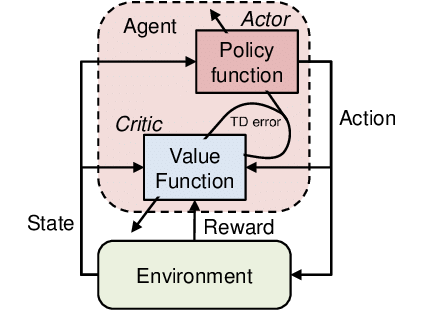
\includegraphics[width=0.5\textwidth]{figures/images/actor_critic_architecture.png}
  \caption[Actor-critic architecture]{Components and interactions in the actor-critic method \cite{fuji2018deep}}
  \label{fig:actor_critic_architecture}
\end{figure}


\section{Deep Reinforcement Learning} \label{sec:deep_rl_background}

As the name suggests, deep reinforcement learning is the combination of deep
learning and reinforcement learning. \autoref{fig:deep_rl} shows the general
architecture of a deep reinforcement learning algorithm; the agent contains a
neural network which determines the next action to be taken, and the agent
interacts with the environment receiving rewards and updating the neural
network.

\begin{figure}[H]
  \centering
  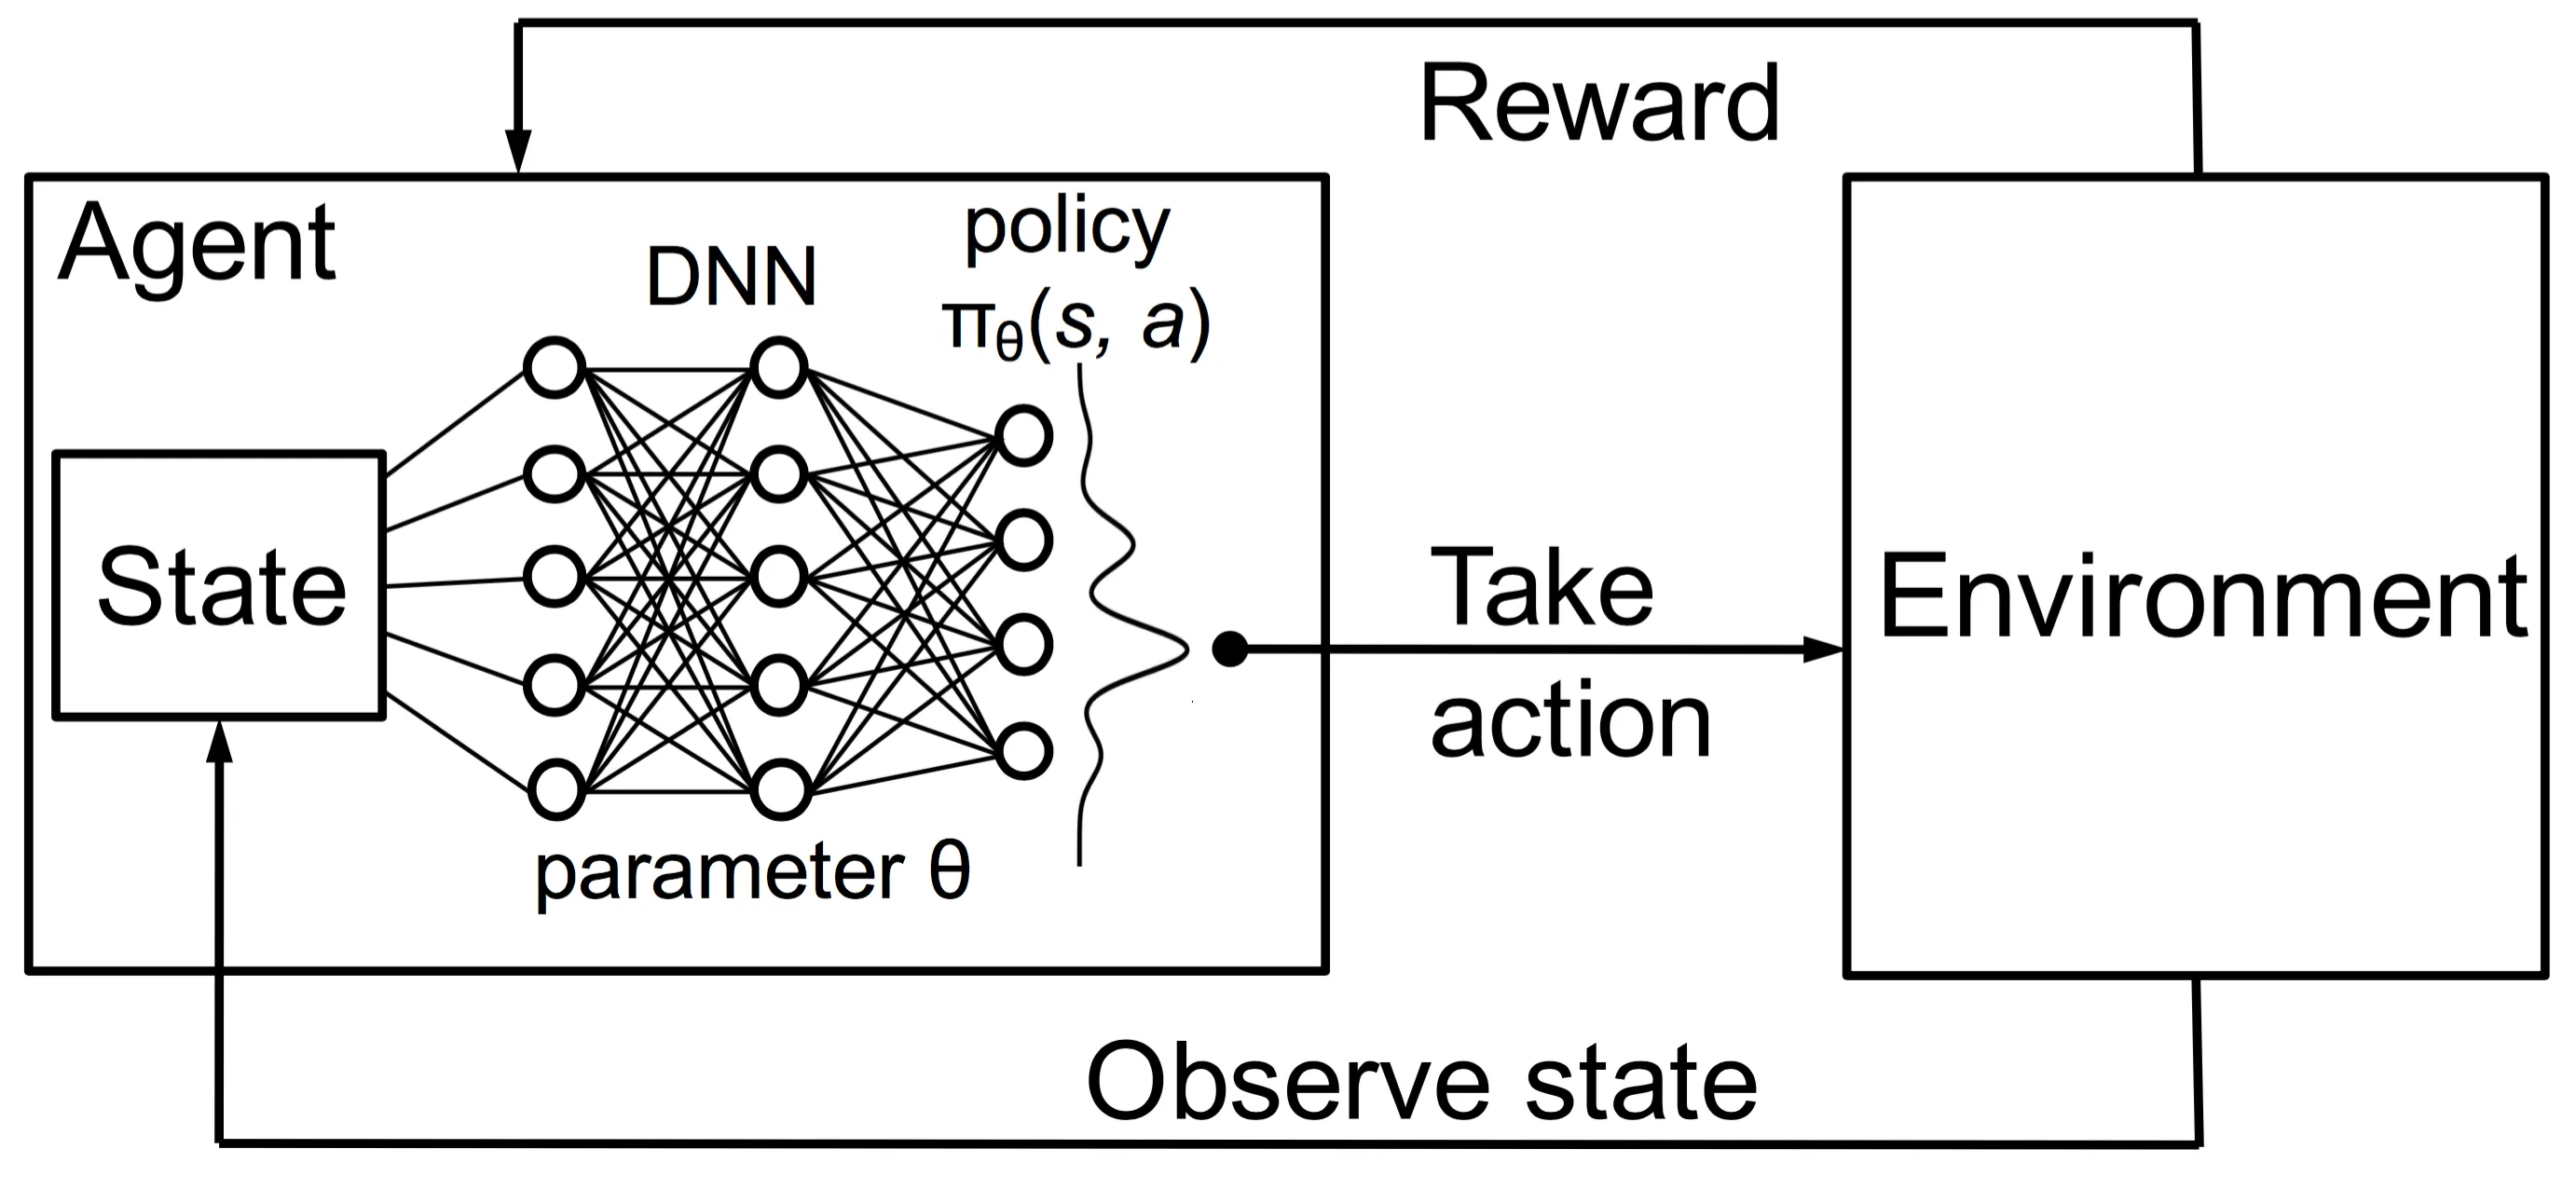
\includegraphics[width=0.6\textwidth]{figures/images/deep_rl.png}
  \caption[Deep reinforcement learning flow]{Deep reinforcement learning components and data flow, showing the interaction between the agent and environment \cite{jakhar2020reinforcement}}
  \label{fig:deep_rl}
\end{figure}


Traditional reinforcement learning methods, as described in
\autoref{sec:reinforcement_learning}, use tabular methods to approximate the
state-value or action-value function; this table becomes too large when the
observation and action space increase in size. Simple function approximators
such as linear functions can be used, although it can be very difficult to
capture the nuances of the environment using these methods.

We can overcome this obstacle with deep reinforcement learning, by instead
using a neural network to approximate the functions necessary for the chosen
algorithm; deep neural networks can handle high dimensional input, and their
size doesn't scale directly with the size of the observation and action space,
unlike tabular methods.

\chapter{Design \& Implementation} \label{chp:design_implementation}
This chapter explores the design and specific techniques used in this project.
We first look at the overall system architecture, and then dive deeper into the
chosen reinforcement learning algorithms, agents, neural networks, and
graphical user interface.

\section{Architecture}
This section describes the architectural design of the implementation. The
system consists of two overarching components: the graphical user interface
(GUI), and the Python notebooks used to train the models. There are two shared
folders used by both the user interface and training notebooks. Additionally,
there is a suite of utilities that is shared between all of the components,
\lstinline{utils.py}, for operations such as logging, file load and save
functions, and string processing functions.

We can see the connections between these components and the data flow in
\autoref{fig:project_schematic}; the filled arrowheads represent data flowing
in the specified direction, while the hollow arrowheads represent component and
function calls.

\begin{figure}[H]
  \centering
  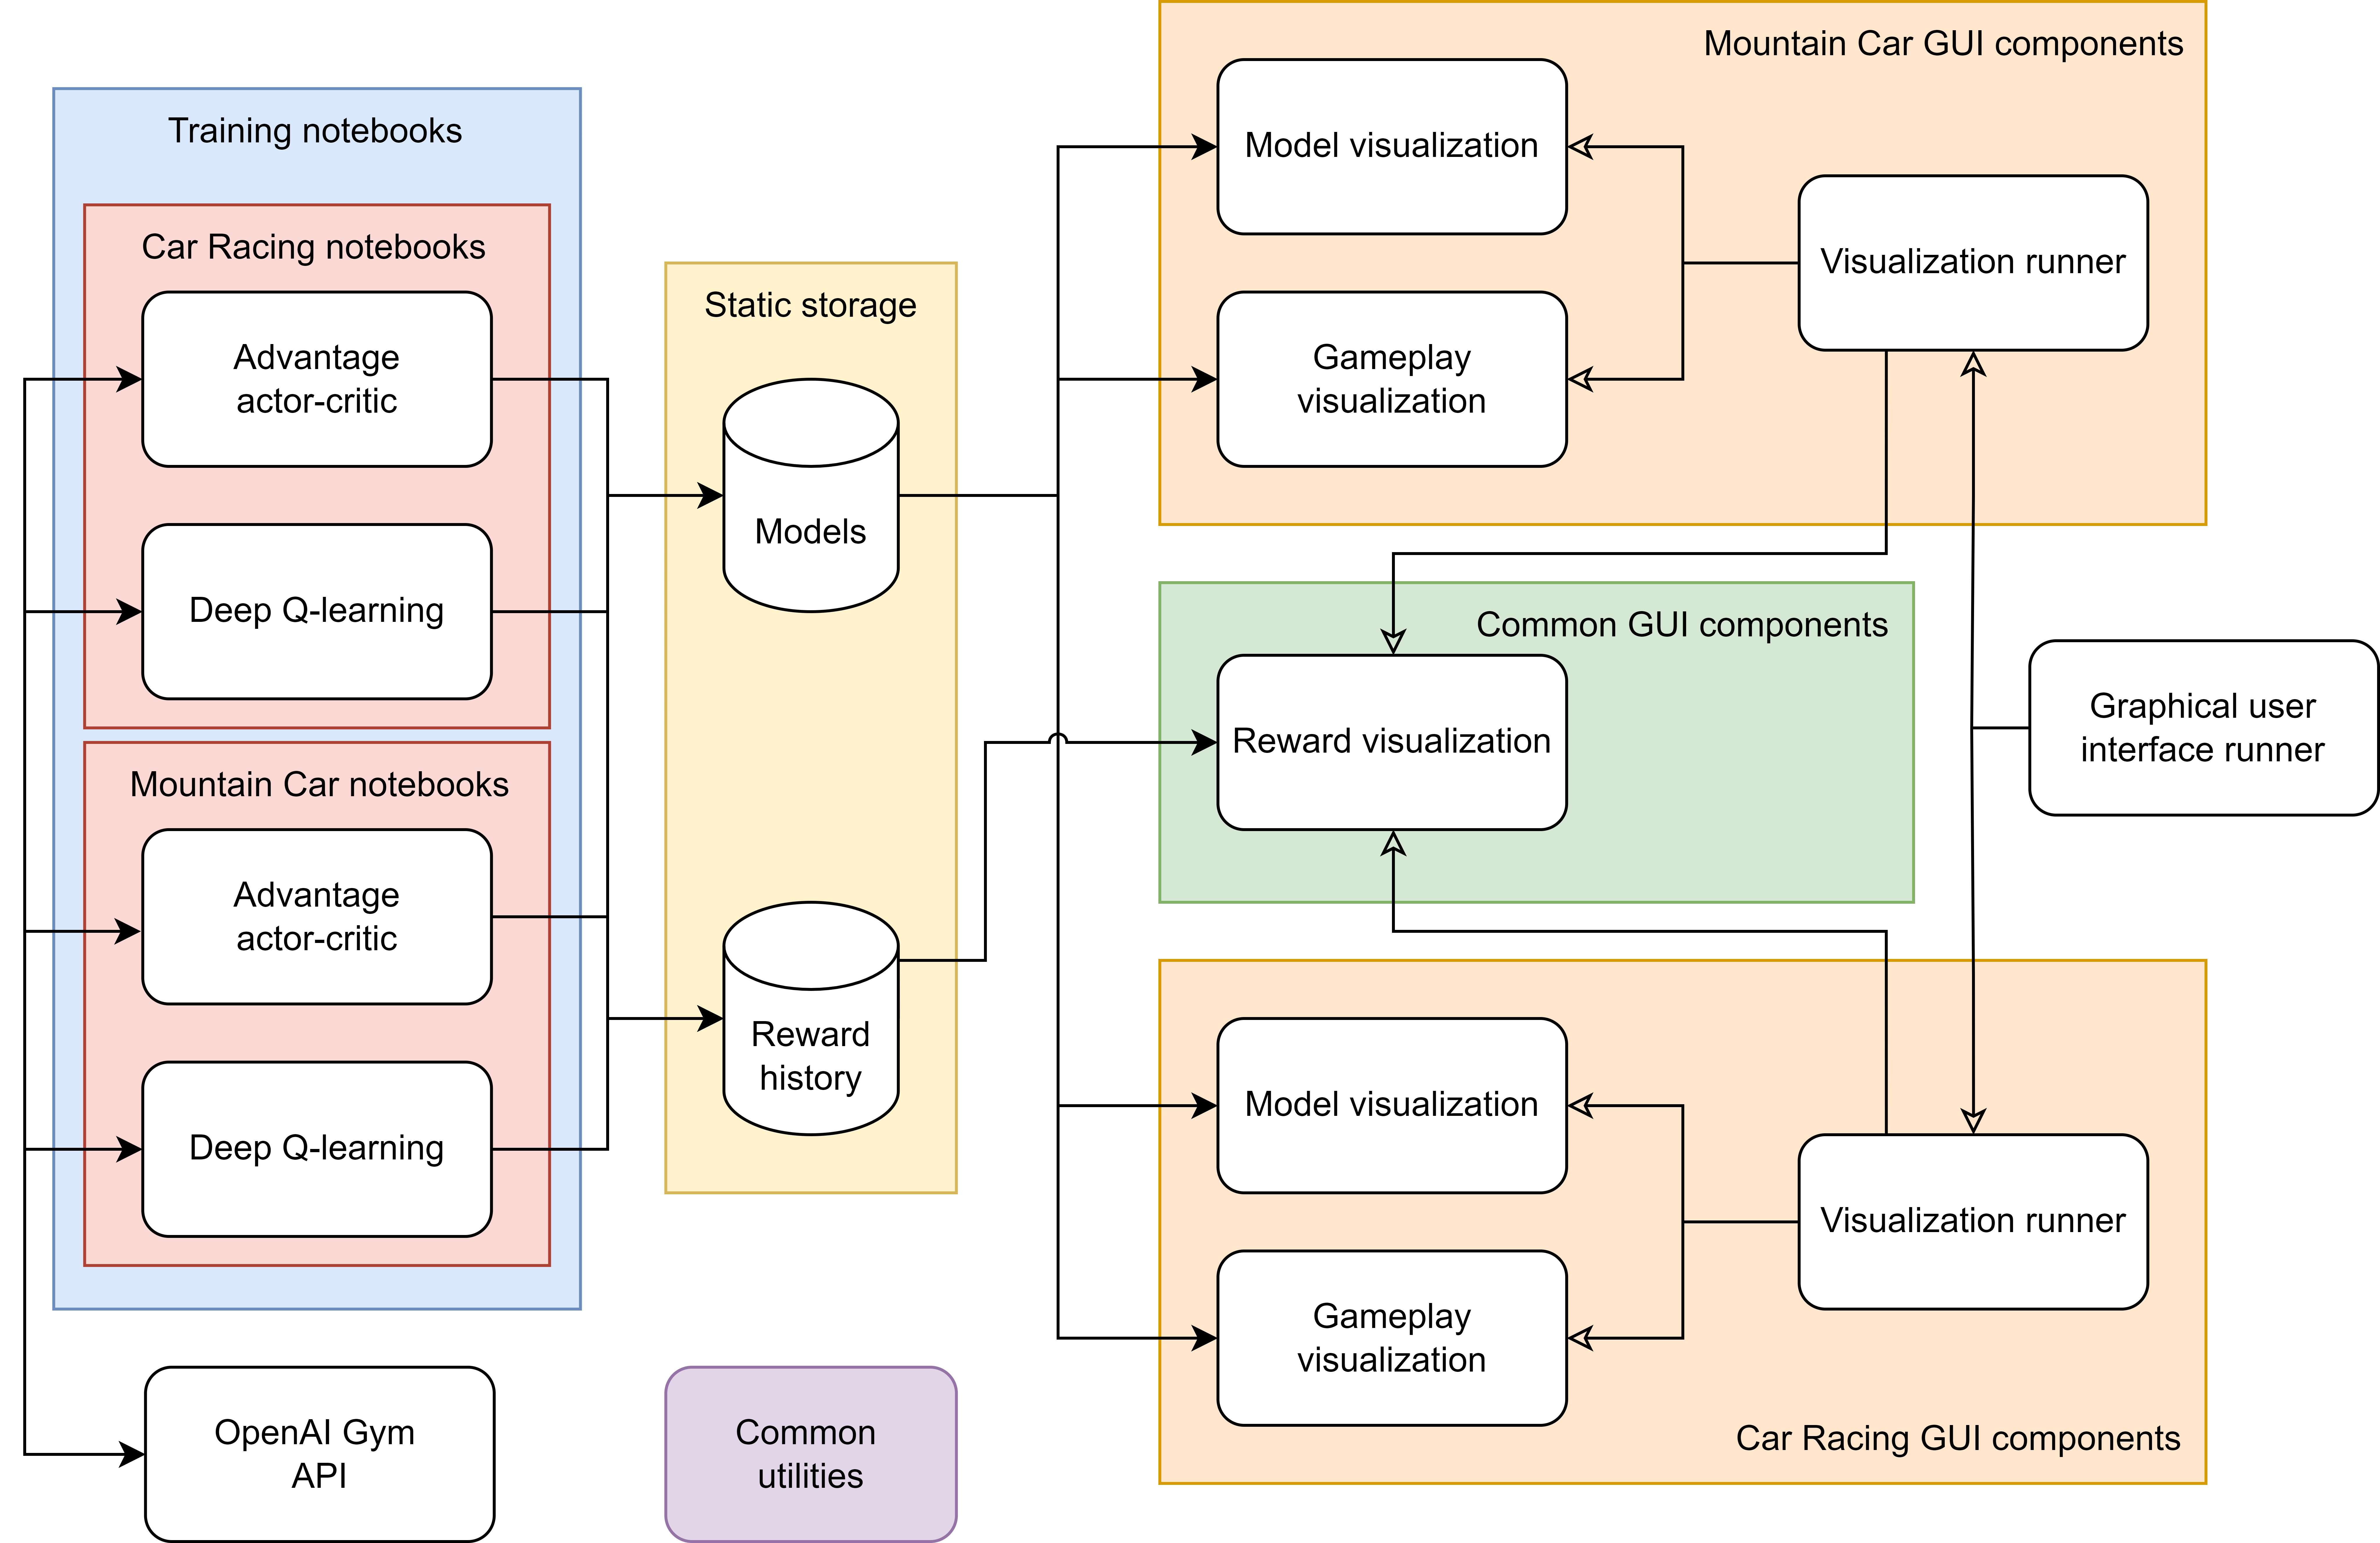
\includegraphics[width=1\textwidth]{figures/images/project_schematic.png}
  \caption[Project architecture schematic]{Schematic of the architecture of the project, showing the components and data flow between the training notebooks and GUI}
  \label{fig:project_schematic}
\end{figure}


\subsection{Training Notebooks}
As the name suggests, the training notebooks are used to train the agents;
there is a separate file for each game-agent pair, as that allows us to fine
tune the code for the relevant environment. The shared functions have been
abstracted to the utilities file, leaving only the core functionality of the
neural network and agent in the respective notebooks. These notebooks use
TensorFlow 2 to implement the neural networks, and they use the Gym API to
facilitate the agent's interactions with the environment; this process is
explained further in \autoref{sec:gym_environment}.

\subsection{Shared File Storage}
The training notebooks and user interface share two common storage folders:
\lstinline{models} and \lstinline{reward_history}. The Python notebooks produce
\lstinline{.h5} model files, which are the saved Keras models representing the
network's weights and any other data required to recreate the exact same model
when loaded. The notebooks also produce \lstinline{.npy} files, which contain a
numpy array of the total reward from every episode during training; this allows
us to plot visualizations containing a reward history graph with a slider to
control the rolling average window size.

\subsection{Graphical User Interface}
We have a master graphical user interface runner file, \lstinline{gui.py},
which calls separate user interface runners for each of the games; this was
required due to the differences between the games and therefore the differences
in network architectures. When the user selects a visualization, the
corresponding files read the required data from the shared folders and display
the selected visualization. This is described in further detail in
\autoref{sec:visualization_design}.

\subsection{Environment}

\subsubsection{Conda}
In order to ensure consistency and reliability during the development process,
we used a \lstinline{conda} environment to run the project. This allowed us to
install the required version of Python and the imported packages, without
interference from an existing Python installation on the machine.

\subsubsection{OpenAI Gym} \label{sec:gym_environment}

This project uses Gym, a Python toolkit developed by OpenAI that provides a
standardized environment for training and testing ML models. It also provides
implementations for both of the chosen games, and many more classic control
games and complex environments \cite{brockman2016gym}. The efficiency and
extensibility of this library allows us to focus on the implementation of the
neural networks and the experimentation of the hyperparameters.

The Python code in \autoref{lst:mountain_car_environment} shows basic usage of
the API to create and interact with the Mountain Car environment. The
environment is first initialized with the selected game, and it is reset for
each episode. We have the option to set a seed for testing to ensure equal
environments and starting states for both agents, although we would like
randomness during training for generalization in newly generated environments.
We pass the state to our agent, which then chooses an action. This is used to
step through the environment, until the game is solved, or the maximum number
of timesteps is reached, as described in \autoref{sec:mountain_car_background}
and \autoref{sec:car_racing_background}. After the episode is finished, the
environment is closed.

\begin{lstlisting}[style=codestyle, basicstyle=\ttfamily\footnotesize, caption={Using OpenAI Gym with the Mountain Car environment}, label=lst:mountain_car_environment]
import gym

EPISODES = 500

env = gym.make("MountainCar-v0")

for e in range(EPISODES):
    # Reset the environment and variables for each episode
    state = env.reset()
    t = 0
    done = False
    total_reward = 0

    while not done:
        # Randomly sample the action space
        action = env.action_space.sample()

        # Take the action
        next_state, reward, done, info = env.step(action)

        state = next_state
        total_reward += reward
        t += 1

    print(f"Episode {e+1} finished after {t} timesteps "
          f"with {total_reward} reward")

env.close()
\end{lstlisting}


Both environments use a discrete action space; this is a conscious decision, as
the DQN algorithm can't work with continuous action spaces, while A2C can.
Choosing discrete variations of the games instead of the continuous ones
ensures both algorithms are trained and tested under the exact same conditions.
Due to the difference in the input and output space of the games, separate
agents are used for each game.

Since one of the primary aims of this project is to decrease training time for
the neural networks, we set the hyperparameter for the maximum number of
episodes to 500.

\section{Deep Q-Learning}
As the name suggests, deep Q-learning is the combination of Q-learning with
deep neural networks; these networks are used as function approximators for the
Q-value function. \autoref{fig:q_vs_dq} shows the difference between both of
these techniques.

\begin{figure}[H]
  \centering
  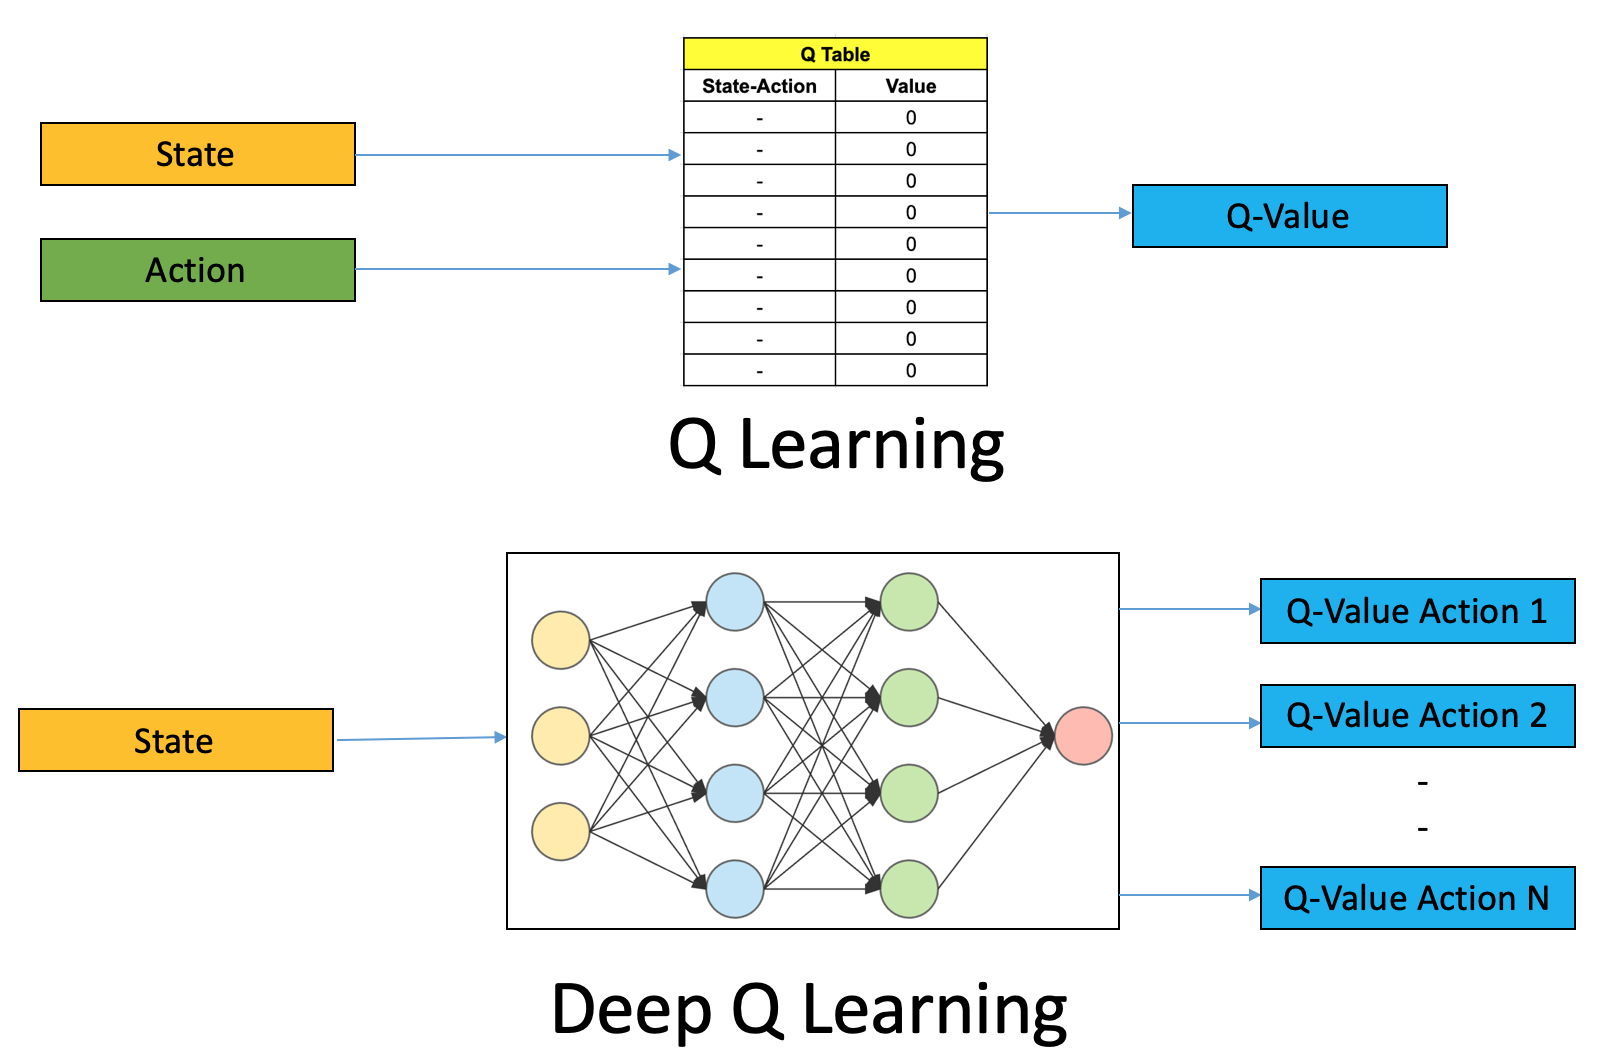
\includegraphics[width=0.7\textwidth]{figures/images/q_vs_dq.png}
  \caption[Q-learning vs deep Q-learning]{Comparison between Q-learning and deep Q-learning, showing their different structures and outputs  \cite{vidhya2019introduction}}
  \label{fig:q_vs_dq}
\end{figure}


\newpage

We use $\theta$ to represent the neural network's weights. We need to define a
loss function in order to update the weights and train the neural network.

\begin{definition}
  The \textit{loss function}
  $$L(\theta)=\mathbb{E}\left[\left(r_t+\gamma\cdot\max_{a_{t+1}}Q(s_{t+1},~a_{t+1};~\theta)-Q(s_{t},~a_{t};~\theta)\right)^{2}\right]$$
  \begin{itemize}[label={}]
    \item $Q(s_t,~a_t;~\theta)$, Q-value for state-action pair
    \item $r_t$, immediate reward
    \item $\gamma$, discount factor of future reward
    \item $\max\limits_{a_{t+1}} Q(s_{t+1},~a_{t+1};~\theta)$, estimate of optimal future reward for next state
  \end{itemize}
\end{definition}

The loss function is the same as the square of the TD error, defined in
\autoref{def:td_error_q_learning}. Taking the derivative of the loss function
with respect to the network weights gives us a gradient, which can be
optimized.

\begin{definition}
  The \textit{gradient}
  $$\frac{\partial{L(\theta)}}{\partial
      \theta}=\mathbb{E}\left[\left(r_t+\gamma\cdot\max_{a_{t+1}}Q(s_{t+1},~a_{t+1};~\theta)-Q(s_{t},~a_{t};~\theta)\right)\frac{\partial{Q(s_{t},~a_{t};~\theta)}}{\partial\theta}\right]$$
\end{definition}

\subsection{Epsilon Greedy} \label{sec:epsilon_greedy}
$\epsilon$-greedy is a commonly used exploration technique for balancing the exploration-exploitation
tradeoff in off-policy algorithms. The hyperparameter $\epsilon$ is used to
determine the probability with which the agent explores. An action $a$ is selected as follows:

$$
  a =
  \begin{cases}
    \underset{a~\in~A}{\arg\max}~Q(a) & \text{with probability } 1-\epsilon \\
    \text{a random action }           & \text{with probability } \epsilon
  \end{cases}
$$

The value of $\epsilon$ decays as the number of episodes increases; it
eventually reaches a lower bound value, where it stays for the rest of the
training process.

The idea behind decaying $\epsilon$ is that the agent becomes more confident in
its policy as training progresses, slowly reducing the need to choose random
actions. An example of a decay graph is shown in \autoref{fig:epsilon_decay}.

\begin{figure}[H]
  \centering
  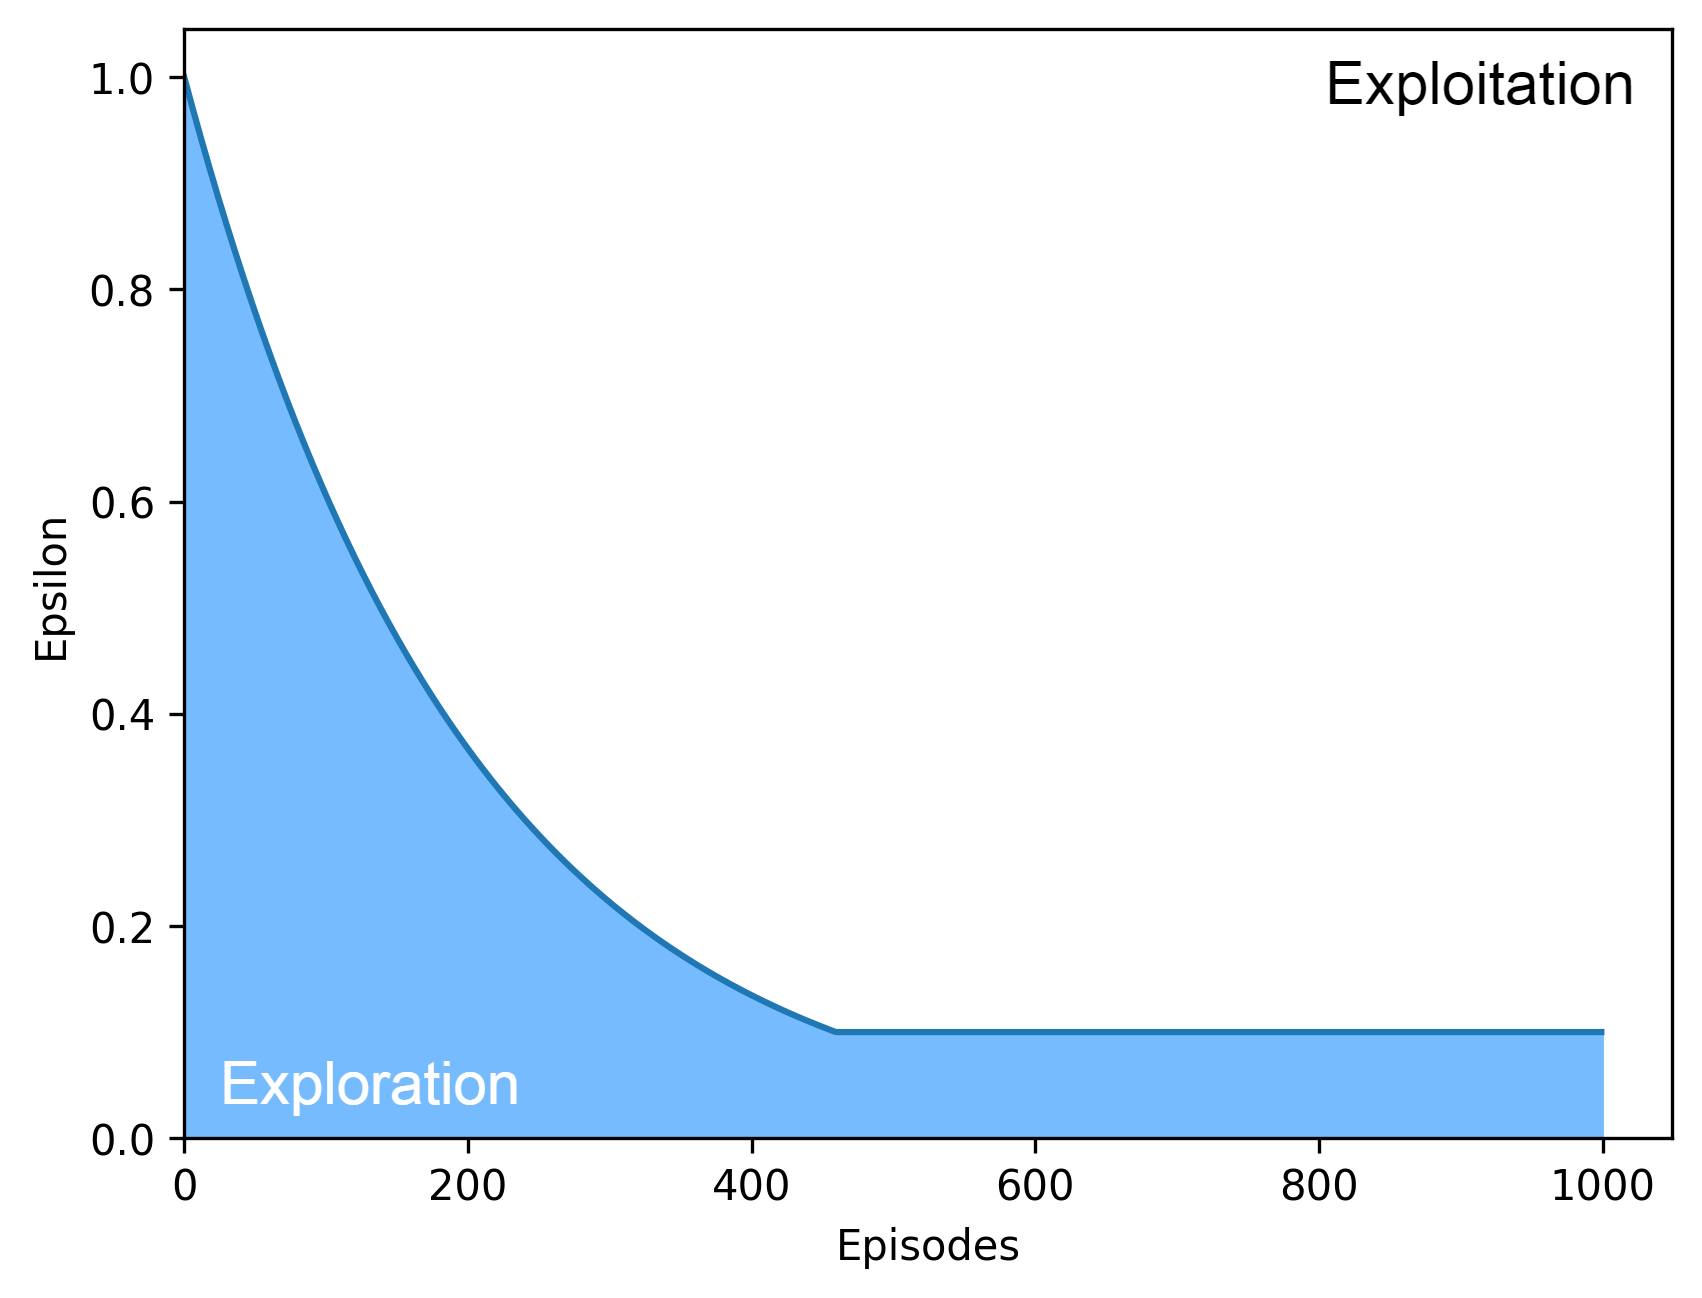
\includegraphics[width=0.6\textwidth]{figures/images/epsilon_decay.png}
  \caption[Epsilon decay graph]{Graph showing an $\epsilon$-decay multiplier of 0.995 every episode with minimum $\epsilon=0.1$, over 1000 episodes}
  \label{fig:epsilon_decay}
\end{figure}


\subsection{Experience Replay} \label{sec:experience_replay}

Experience replay is a technique used to improve the efficiency and stability
of the training process. Instead of using each experience\footnote{Experience
  refers to a transition from one state to another, and the associated action and
  reward} only once, this technique involves storing the agent's experiences in a
replay buffer $\mathcal{D}$. These experiences are then uniformly sampled in
minibatches during training, $U(\mathcal{D})$, which allows the agent to learn
from experiences that occurred in different parts of the state space, helping
with the network's generalization for new situations as it is not simply
learning from successive experiences. Improving generalization also helps with
the moving targets problem, described in earlier in
\autoref{sec:on_vs_off_policy}. We can provide an updated definition for our
loss function, incorporating experience replay.

\begin{definition}
  The \textit{loss function with experience replay}
  $$L(\theta)=\mathbb{E}_{(s_t,~a_t,~r_t,~s_{t+1})~\thicksim ~U(\mathcal{D})}\left[\left(r_t+\gamma\cdot\max_{a_{t+1}}Q(s_{t+1},~a_{t+1};~\theta)-Q(s_{t},~a_{t};~\theta)\right)^{2}\right]$$
\end{definition}

This project implements uniformly sampled experience replay, the technique
described above, as it provides excellent results \cite{mnih2013playing}. There
are many advanced variations of experience replay, including prioritized
experience replay \cite{schaul2015prioritized} and hindsight experience replay
\cite{andrychowicz2017hindsight}, which optimize this method further.

Below, we can see both a schematic and code implementation of the deep Q
learning algorithm, including all of the aforementioned improvements.

\begin{figure}[H]
  \centering
  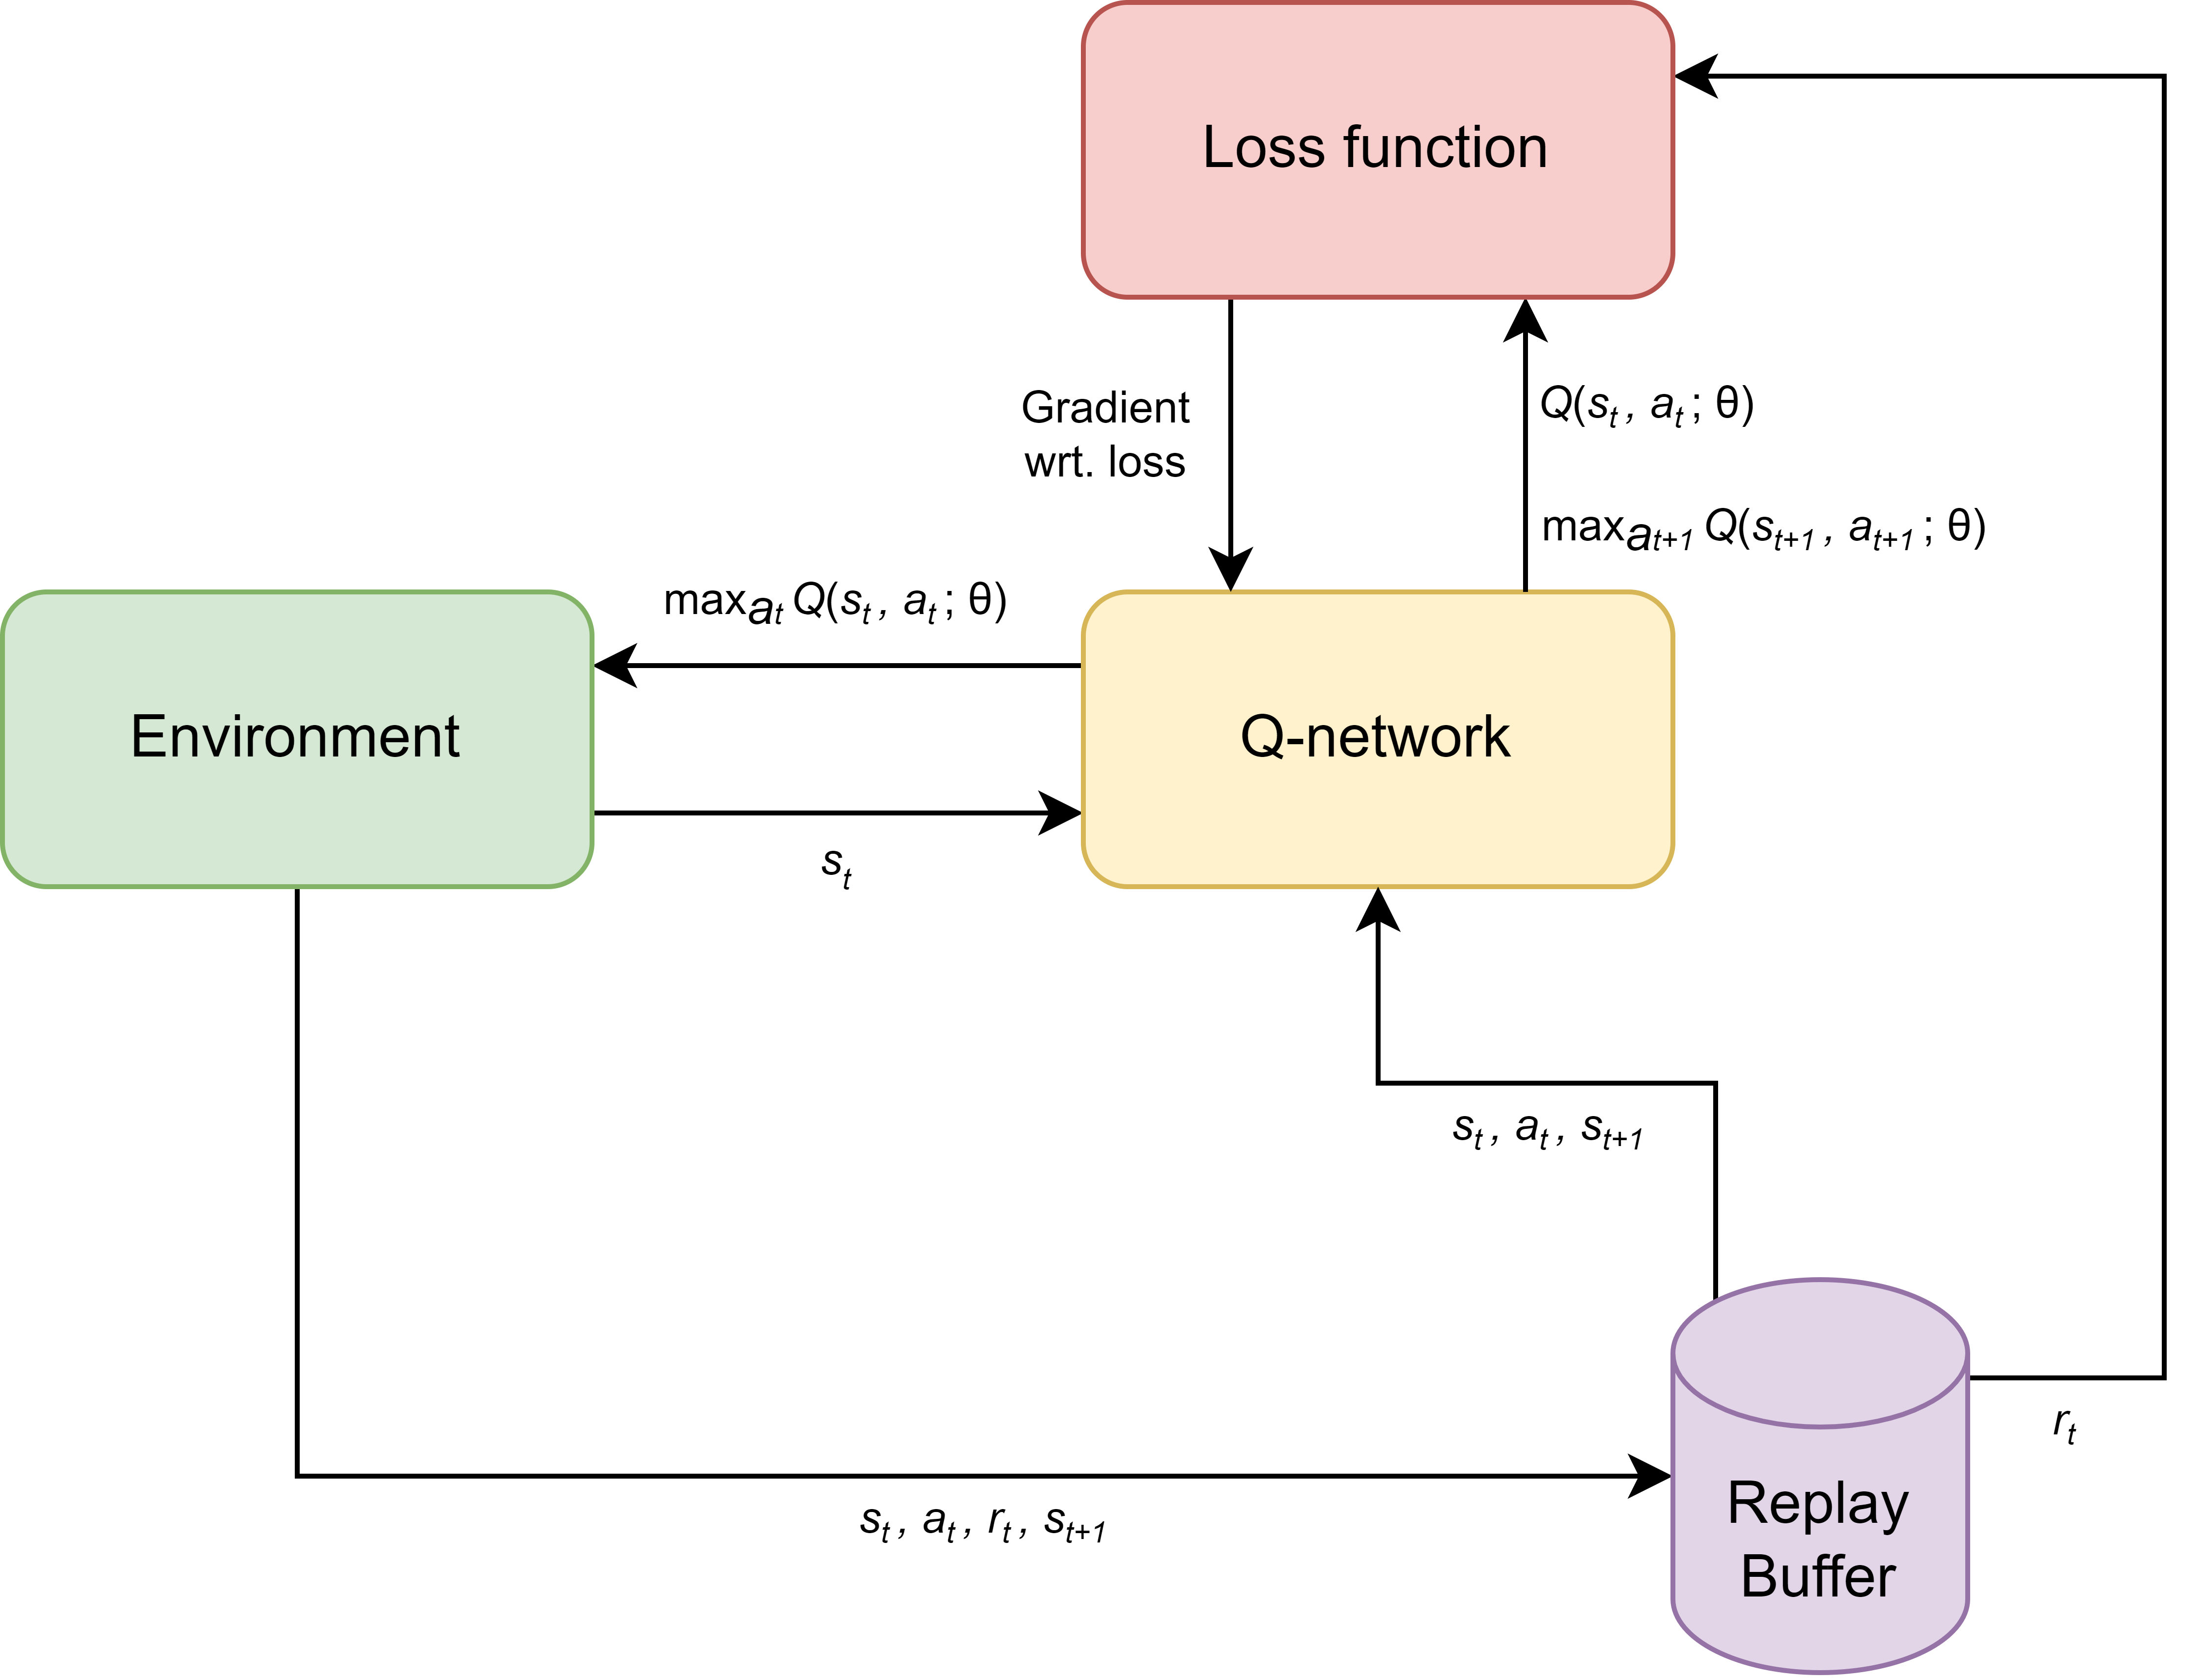
\includegraphics[width=0.8\textwidth]{figures/images/dqn_architecture.png}
  \caption[Deep Q-learning architecture]{Components and their interactions in the deep Q-learning algorithm with experience replay}
  \label{fig:dqn_architecture}
\end{figure}


\begin{algorithm}[H]
  \caption[Deep Q-Learning]{Deep Q-Learning with Experience Replay}
  \label{alg:deep_q_learning}
  \begin{algorithmic}
    \State Initialize Q-network with random weights $\theta$
    \For{episode $i$ in $1:N$}
    \State Set initial state $s_t$
    \While{$s_t$ is not terminal}
    \State{
      $
        a_t =
        \begin{cases}
          \max\limits_{a_t} Q(s_t, a_t;~\theta) & \text{with probability } 1-\epsilon \\
          \text{a random action }               & \text{with probability } \epsilon
        \end{cases}
      $
    }
    \State Take action $a_t$ and observe reward $r_t$ and new state $s_{t+1}$
    \State Store transition $(s_t,~a_t,~r_t,~s_{t+1})$ in $\mathcal{D}$
    \State Sample a random batch of transitions $(s_j,~a_j,~r_j,~s_{j+1})$ from $\mathcal{D}$
    \State{
      $
        y_j =
        \begin{cases}
          r_j                                                              & \text{for terminal } s_{j+1}     \\
          r_j +\gamma\cdot\max\limits_{a_{j+1}}Q(s_{j+1},~a_{j+1};~\theta) & \text{for non-terminal } s_{j+1}
        \end{cases}
      $
    }
    \State Perform gradient descent on $(y_j - Q(s_j,a_j;~\theta))^2$ wrt. the network weights $\theta$
    \State Update state $s_t \gets s_{t+1}$
    \EndWhile
    \EndFor
  \end{algorithmic}
\end{algorithm}


\newpage

\section{Advantage Actor-Critic}

Advantage actor-critic (A2C) is an instance of the actor-critic method, using
neural networks to approximate the actor and critic functions. We make some
improvements to the generic one-step actor-critic algorithm, by using entropy
regularization to encourage exploration, discussed in
\autoref{sec:entropy_regularization}. A2C was chosen due to its stability and
sample-efficiency compared to similar algorithms, such as Asynchronous
Advantage Actor-Critic (A3C) \cite{wu2017scalable}. We can define an advantage
function, which in the case of the one-step algorithm is equivalent to the TD
error in \autoref{def:td_error_actor_critic}.

\begin{definition} \label{def:td_error_a2c}
  The \textit{advantage}
  $$A(s_t, a_t) = r_t+\gamma\cdot V(s_{t+1}) - V(s_t)$$
  \begin{itemize}[label={}]
    \item $r_t$, immediate reward
    \item $\gamma$, discount factor of future reward
          \begin{itemize}[label={}]
            \item $\gamma\in[0,1]$
          \end{itemize}
    \item $V(s_t)$, estimate of cumulative reward from current state
    \item $V(s_{t+1})$, estimate of cumulative reward from next state
  \end{itemize}
\end{definition}

We can use this advantage function to compute the losses for both the actor and
the critic.

\begin{definition}
  The \textit{actor loss function}
  $$L_{actor}=-\log (\pi(a_t~|~s_t)) \cdot A(s_t, a_t)$$
\end{definition}

\begin{definition}
  The \textit{critic loss function}
  $$L_{\text{critic}} = A(s_t, a_t)^2$$
\end{definition}

\subsection{Stochastic Policy Exploration}
By using a stochastic policy rather than the deterministic variant, we
encourage the agent to explore, as we select an action based on the weighted
probability rather than taking the action with the maximum probability, like in
the Q-learning methods. The policy is initialized with random values, allowing
this technique to increase the probability of the agent exploring with new
state-action pairs in the beginning of the training process.

\subsection{Entropy Regularization} \label{sec:entropy_regularization}
Entropy regularization further encourages exploration by adding an entropy term
to the loss function of the actor, which is derived from the probability
distribution over the actions. This entropy term "flattens" the distribution,
forcing exploration by increasing the chances of an action with a lower
probability according to the actor network being chosen.

\begin{definition}
  The \textit{entropy} of the policy distribution
  $$H_t=-\log(\pi(a_t~|~s_t)) \cdot \pi(a_t~|~s_t)$$
\end{definition}

\begin{definition}
  The \textit{actor loss function with entropy regularization}
  $$L_{actor}=-\log (\pi(a_t~|~s_t)) \cdot A(s_t, a_t) - \beta\cdot H_t$$
\end{definition}

$\beta$ represents the entropy coefficient; a value of 0 means that no entropy regularization is used. As we increase this value, we increase the amount of regularization applied. The factor
is a hyperparameter optimized during training, with common values being
$\beta\in[0.01,0.50]$. We can see a visual representation of this in \autoref{fig:entropy_regularization}.

\begin{figure}[H]
  \captionsetup[subfigure]{justification=centering}
  \centering
  \begin{subfigure}[t]{0.47\linewidth}
    {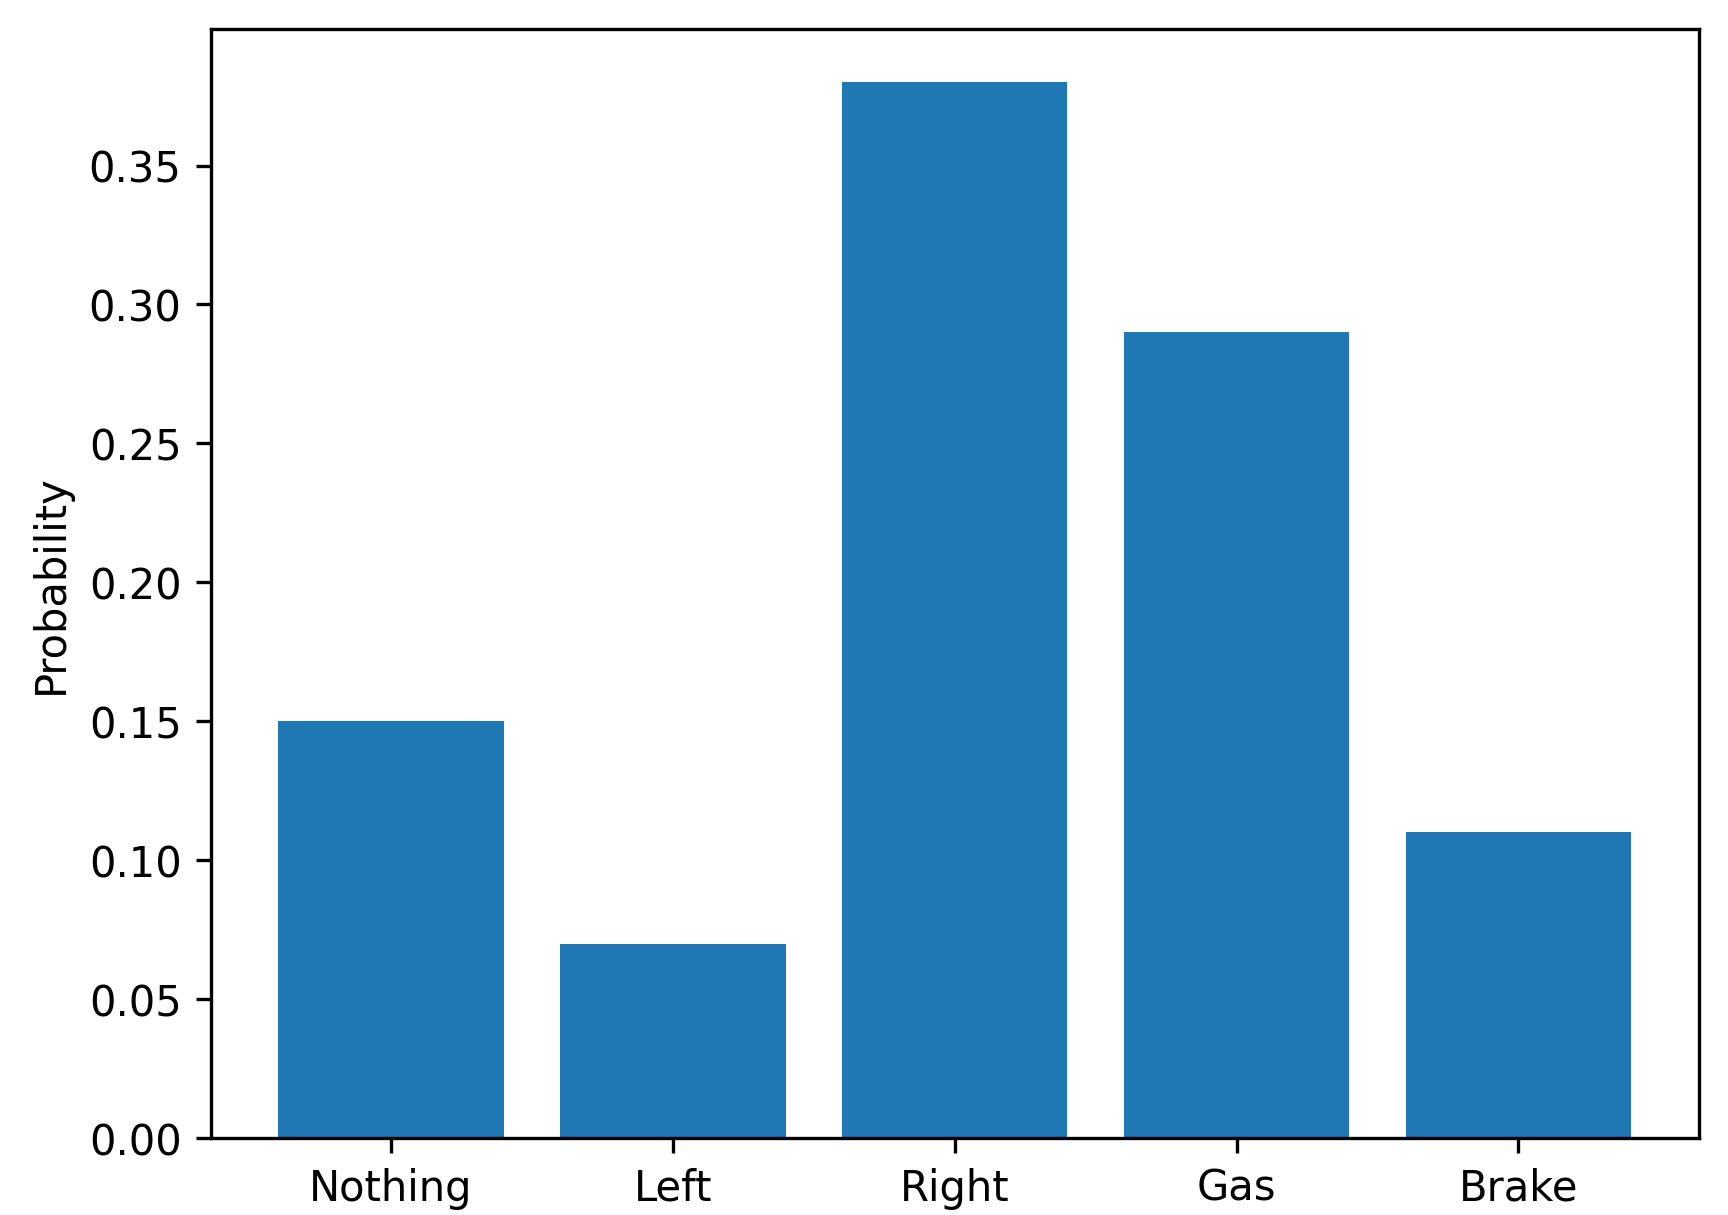
\includegraphics[height=5cm]{figures/images/unregularized.png}}
    \caption{Without regularization}
  \end{subfigure}
  \hfill
  \begin{subfigure}[t]{0.47\linewidth}
    {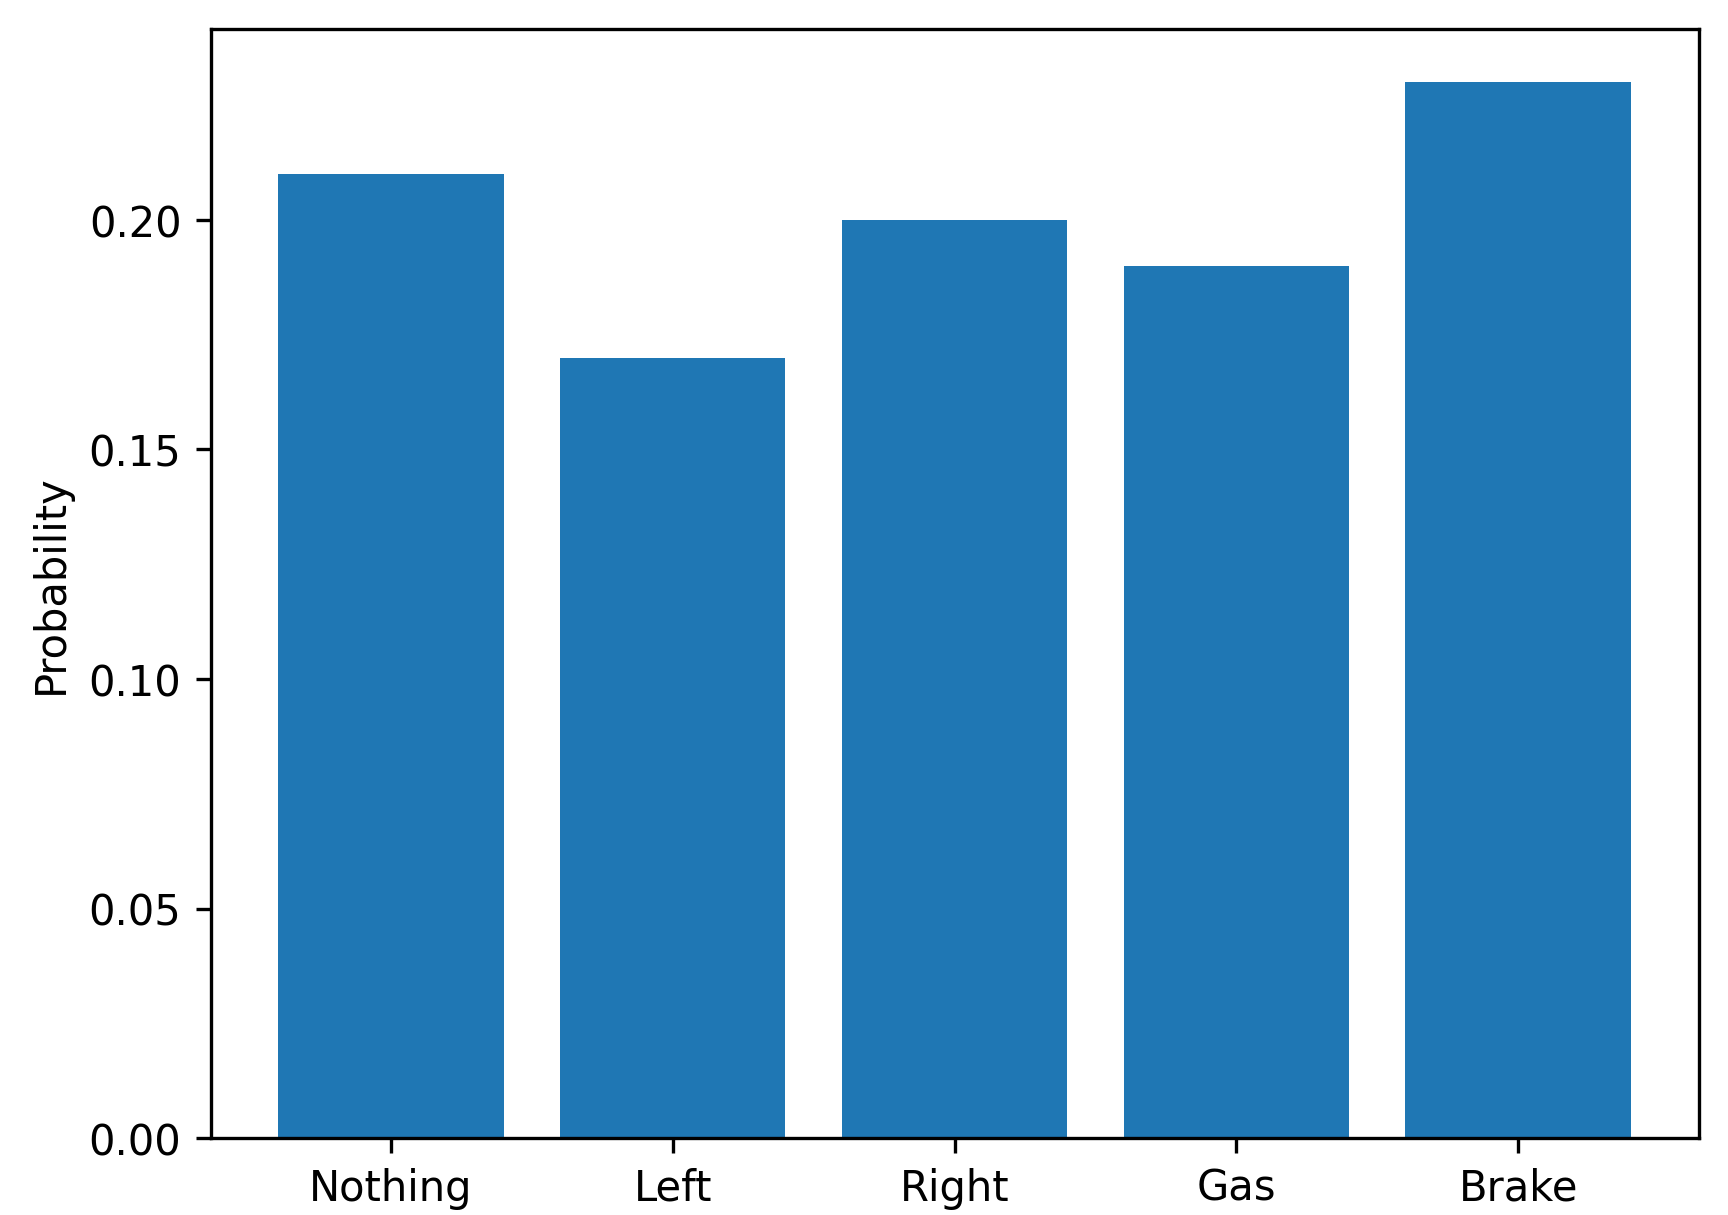
\includegraphics[height=5cm]{figures/images/regularized.png}}
    \caption{With regularization}
  \end{subfigure}
  \caption[Entropy regularization graphs]{Example of entropy regularization actor output for Car Racing}
  \label{fig:entropy_regularization}
\end{figure}


Below, we have the pseudocode for the advantage actor-critic algorithm with
entropy regularization.

\begin{algorithm}[H]
  \caption[Advantage Actor-Critic]{Advantage Actor-Critic with Entropy Regularization}
  \label{alg:advantage_actor_critic}
  \begin{algorithmic}
    \State Initialize actor network with random weights $\theta_{actor}$
    \State Initialize critic network with random weights $\theta_{critic}$
    \For{episode $i$ in $1:N$}
    \State Set initial state $s_t$
    \While{$s_t$ is not terminal}
    \State Select action $a_t$ from policy $\pi_{\theta_{actor}}(a_t~|~s_t)$ using weighted random sampling
    \State Take action $a_t$ and observe reward $r_t$ and new state $s_{t+1}$
    \State Compute advantage $A(s_t, a_t) \gets r_t+\gamma\cdot V(s_{t+1}) - V(s_t)$
    \State Compute entropy $H_t\gets-\log(\pi(a_t~|~s_t)) \cdot \pi(a_t~|~s_t)$
    \State Perform gradient descent on $-\log (\pi(a_t~|~s_t)) \cdot A(s_t, a_t) - \beta\cdot H_t$
    \State \hspace{1cm} wrt. the actor network weights $\theta_{actor}$ and update network
    \State Perform gradient descent on $A(s_t, a_t)^2$
    \State \hspace{1cm} wrt. the critic network weights $\theta_{critic}$ and update network
    \State Update state $s_t \gets s_{t+1}$
    \EndWhile
    \EndFor
  \end{algorithmic}
\end{algorithm}


\section{Agents}

This section outlines the implementation details of the agents, and it includes
the design of the neural networks; they have been implemented in Python 3.7
exactly as described in \autoref{alg:deep_q_learning} and
\autoref{alg:advantage_actor_critic}.

The network structure was not the basis of experimentation, so it was kept
relatively constant during the evaluation process. Model architectures were
inspired and adapted from other applications with similar input and output
structures.

The networks used in this project were trained using the "Adam" gradient
descent optimizer, as it has been shown to outperform alternative methods such
as stochastic gradient descent (SGD) and RMSProp \cite{kingma2014adam}.

\subsection{Mountain Car}

\subsubsection{Neural Networks}
Data is received from the environment, and it is inputted directly into the
dense (fully connected) layers of the neural network. For Mountain Car, three
layers were used for the Q-network and actor network, and two layers were used
for the critic network. We can see the networks' details in the tables below.

\begin{table}[H]
  \centering
  \begin{tabular}{|c|c|c|c|c|c|c|}
    \hline
    \textbf{Layer} & \textbf{Input} & \textbf{Activation} & \textbf{Output} \\
    \hline
    Dense          & 2              & ReLU                & 32              \\
    Dense          & 32             & ReLU                & 64              \\
    Dense          & 64             & ReLU                & 3               \\
    \hline
  \end{tabular}
  \caption[Mountain Car DQN structure]{Mountain Car deep Q-network layers and parameters}
  \label{table:mountain_car_dqn}
\end{table}


\begin{table}[H]
  \centering
  \subfloat[Actor]{
    \begin{tabular}{|c|c|c|c|c|c|c|}
      \hline
      \textbf{Layer} & \textbf{Input} & \textbf{Activation} & \textbf{Output} \\
      \hline
      Dense          & 2              & ReLU                & 32              \\
      Dense          & 32             & ReLU                & 64              \\
      Dense          & 64             & ReLU                & 3               \\
      \hline
    \end{tabular}
  }
  \subfloat[Critic]{
    \begin{tabular}{|c|c|c|c|c|c|c|}
      \hline
      \textbf{Layer} & \textbf{Input} & \textbf{Activation} & \textbf{Output} \\
      \hline
      Dense          & 2              & ReLU                & 32              \\
      Dense          & 32             & ReLU                & 1               \\
      \hline
    \end{tabular}
  }
  \caption[Mountain Car A2C network structure]{Mountain Car advantage actor-critic layers and parameters}
  \label{table:mountain_car_a2c}
\end{table}


\subsubsection{Reward Shaping} \label{sec:reward_shaping}

The Mountain Car environment has sparse rewards, so it benefits greatly in
terms of training performance to shape the reward function during training. The
same idea cannot be applied to Car Racing, as we only have access to an image
of the current frame. For this reason, we apply reward shaping in Mountain Car
to improve training speed and final scores.

In Mountain Car, the agent receives a reward of -1 for every timestep, without
any indication on performance until the episode is finished, or the goal is
reached. This means that learning is greatly diminished, as the agent can not
learn anything meaningful in the timesteps before the end of the episode. To
combat this issue, we can use reward shaping to guide the agent towards the
goal. We define a reward shaping function as shown in
\autoref{lst:reward_shaping}.

\begin{lstlisting}[style=codestyle, basicstyle=\ttfamily\footnotesize, caption={Mountain Car reward shaping}, label=lst:reward_shaping]
def shape_reward(state, next_state, reward):
  return reward + 300 * (abs(next_state[1]) - abs(state[1]))
\end{lstlisting}


This reward function takes into account the speed of the car before and after
the action, \lstinline{state[1]} and \lstinline{next_state[1]} respectively. By
adding the scaled difference in speed to the reward, the agent is incentivized
to gain more speed than had previously. The multiplier value 300 was found to
produce the highest scores after training.

\subsection{Car Racing}

\subsubsection{Frame Skipping}

A very important aspect of this environment is the idea of using a frame skip.
Without frame skipping, the frames in the frame stack are very similar as they
are consecutive, so they provide little information to the neural network about
the car's dynamics. To combat this, the agent repeats the action chosen $n + 1$
times instead of just once, and only the final state observed is added to the
frame stack. This means that consecutive images on the frame stack are further
apart in the game, and provide more information to the network about the car.
This is shown in visually \autoref{fig:frame_skip}. We can define a
\mbox{\lstinline{take_action()}} function as shown in \autoref{lst:frame_skipping}
and call this function instead of directly calling \lstinline{env.step()} in
the main episode loop for the Car Racing agents.

\begin{figure}[H]
  \centering
  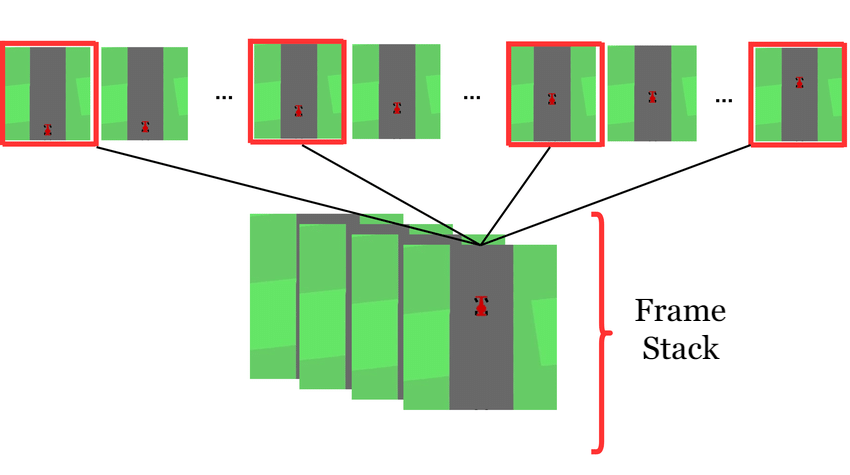
\includegraphics[width=0.75\textwidth]{figures/images/frame_skip.png}
  \caption[Car Racing frame skip]{Car Racing frame skip \cite{montoya2021decoupling}}
  \label{fig:frame_skip}
\end{figure}


\newpage

\begin{lstlisting}[style=codestyle, basicstyle=\ttfamily\footnotesize, caption={Car Racing frame skipping}, label=lst:frame_skipping]
def take_action(env, action):
  reward = 0

  for _ in range(FRAME_SKIP + 1):
      next_state, frame_reward, done, info = env.step(action)

      reward += frame_reward
      if done:
          break

  return next_state, reward, done, info
\end{lstlisting}


\subsubsection{Input Preprocessing}

For the Car Racing agent, we need to process the image before it can be passed
to the Dense layers of the network. This section is not applicable for the
Mountain Car environment, as we receive direct data about the car's position
and velocity.

The state returned by the Gym environment is a $96\times 96$ RGB image, which
contains:

\begin{itemize}
  \item A dynamically coloured car at a fixed coordinate position in the image
  \item A polychromatic gray track and green grass surrounding the track
  \item Red and white curbs on the track corners (not visible in the figure) black
  \item A "dashboard" at the bottom with metadata about the car
\end{itemize}

Most of these details are unnecessary, and would require more extensive and
complex neural networks to extract features relevant to the policy. We can
therefore process the image before passing it to the network. Below are the
steps used in this project for doing so, and their corresponding line of code
in \autoref{lst:car_racing_image_processing}. OpenCV and numpy were used for
this, as shown in the code sample.

\begin{itemize}
  \item \textbf{Desaturation} -- converts the image to greyscale reducing the
        computational load by turning a $96\times 96\times 3$ image to $96\times
          96\times 1$, without losing any necessary detail
  \item \textbf{Masking} -- draws a black box to emphasize the car and
        reduce unwanted interference from the car's details and changing colour between
        episodes
  \item \textbf{Colour homogenization} -- homogenizes the different colour shades of
        the track (including curbs) and grass, which add unnecessary complexity; these
        details are not required to find the optimal policy
  \item \textbf{Cropping} -- crops the "dashboard" area, as it is not required and adds
        an unwanted artefact to the image; the square ratio is maintained by cropping
        the sides of the image, as these areas mostly only contain grass
  \item \textbf{Normalization} -- scales pixel values to be in the range $[0, 1]$,
        helping the optimization algorithm navigate the parameter space
\end{itemize}

\newpage

\begin{lstlisting}[style=codestyle, basicstyle=\ttfamily\footnotesize, caption={Car Racing state image preprocessing}, label=lst:car_racing_image_processing]
def process_state(state):
  # Desaturation
  state = cv2.cvtColor(state, cv2.COLOR_BGR2GRAY).astype(float)

  # Masking
  cv2.rectangle(state, (45, 66), (50, 76), 0, -1)

  # Colour homogenization
  state[np.where((state >= 160) & (state < 180))] = 255
  state[np.where((state >= 90) & (state < 160))] = 100

  # Cropping
  state = state[0:84, 6:90]

  # Normalization
  state /= 255.0

  return state
\end{lstlisting}


The result of this image processing can be seen in
\autoref{fig:car_racing_state_processing}. Note that the grey border is not
part of the image passed to the neural network, and has been added for image
edge clarity.

\begin{figure}[H]
  \centering
  \begin{subfigure}{0.22\linewidth}
    {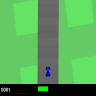
\includegraphics{figures/images/car_racing_state_original.png}}
    \caption{Original state}
  \end{subfigure}
  \qquad\tikz[baseline=-4\baselineskip]\draw[ultra thick,->] (0,0) -- ++ (1,0);\qquad
  \begin{subfigure}{0.2\linewidth}
    \fbox{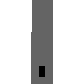
\includegraphics{figures/images/car_racing_state_processed.png}}
    \caption{Processed state}
  \end{subfigure}
  \caption[Car Racing state preprocessing]{Preprocessing of the Car Racing input state image}
  \label{fig:car_racing_state_processing}
\end{figure}


\subsubsection{Neural Networks}

Images are added to the frame stack after they have been preprocessed, and the
entire data structure is passed to the neural network. The frame stack allows
the network to deduce the car's speed and direction, as explained in
\autoref{sec:markov_property}.

The first step performed by the neural networks is a convolution with ReLU
activation, paired with a max pooling layer. This is then repeated once again
with different filter sizes, after which a flatten layer linearizes the data.
The linear data is then passed to the two dense layers of the neural network.

This structure is common across the deep Q-network and both the actor and
critic networks, with the only difference being the output size. Below are
tables with the exact parameters used in the neural networks for both
algorithms.

\begin{table}[H]
  \centering
  \subfloat{
    \small
    \begin{tabular}{|c|c|c|>{\centering\arraybackslash}p{1cm}|c|c|>{\centering\arraybackslash}p{1.5cm}|c|}
      \hline
      \textbf{Layer} & \textbf{Input}        & \textbf{Filters} & \textbf{Filter Size} & \textbf{Stride} & \textbf{Activation} & \textbf{Regular-ization} & \textbf{Output}       \\
      \hline
      Conv           & $84\times 84\times 3$ & 8                & $7\times 7$          & 4               & ReLU                & L2                       & $20\times 20\times 8$ \\
      MaxPooling     & $20\times 20\times 8$ & -                & $2\times 2$          & 2               & -                   & -                        & $10\times 10\times 8$ \\
      Conv           & $10\times 10\times 8$ & 16               & $3\times 3$          & 1               & ReLU                & L2                       & $8\times 8\times 16$  \\
      MaxPooling     & $8\times 8\times 16$  & -                & $2\times 2$          & 2               & -                   & -                        & $4\times 4\times 16$  \\
      Flatten        & $4\times 4\times 16$  & -                & -                    & -               & -                   & -                        & 256                   \\
      Dense          & 256                   & -                & -                    & -               & ReLU                & L2                       & 512                   \\
      Dense          & 512                   & -                & -                    & -               & Linear              & L2                       & 5                     \\
      \hline
    \end{tabular}
  }
  \caption[Car Racing DQN structure]{Car Racing deep Q-network layers and parameters}
  \label{table:car_racing_dqn}
\end{table}


\begin{table}[H]
  \centering
  \subfloat[Actor]{
    \small
    \begin{tabular}{|c|c|c|>{\centering\arraybackslash}p{1cm}|c|c|>{\centering\arraybackslash}p{1.5cm}|c|}
      \hline
      \textbf{Layer} & \textbf{Input}        & \textbf{Filters} & \textbf{Filter Size} & \textbf{Stride} & \textbf{Activation} & \textbf{Regular-ization} & \textbf{Output}       \\
      \hline
      Conv           & $84\times 84\times 3$ & 8                & $7\times 7$          & 4               & ReLU                & L2                       & $20\times 20\times 8$ \\
      MaxPooling     & $20\times 20\times 8$ & -                & $2\times 2$          & 2               & -                   & -                        & $10\times 10\times 8$ \\
      Conv           & $10\times 10\times 8$ & 16               & $3\times 3$          & 1               & ReLU                & L2                       & $8\times 8\times 16$  \\
      MaxPooling     & $8\times 8\times 16$  & -                & $2\times 2$          & 2               & -                   & -                        & $4\times 4\times 16$  \\
      Flatten        & $4\times 4\times 16$  & -                & -                    & -               & -                   & -                        & 256                   \\
      Dense          & 256                   & -                & -                    & -               & ReLU                & L2                       & 512                   \\
      Dense          & 512                   & -                & -                    & -               & Linear              & L2                       & 5                     \\
      \hline
    \end{tabular}
  }
  \vspace{0.8cm}
  \subfloat[Critic]{
    \small
    \begin{tabular}{|c|c|c|>{\centering\arraybackslash}p{1cm}|c|c|>{\centering\arraybackslash}p{1.5cm}|c|}
      \hline
      \textbf{Layer} & \textbf{Input}        & \textbf{Filters} & \textbf{Filter Size} & \textbf{Stride} & \textbf{Activation} & \textbf{Regular-ization} & \textbf{Output}       \\
      \hline
      Conv           & $84\times 84\times 3$ & 8                & $7\times 7$          & 4               & ReLU                & L2                       & $20\times 20\times 8$ \\
      MaxPooling     & $20\times 20\times 8$ & -                & $2\times 2$          & 2               & -                   & -                        & $10\times 10\times 8$ \\
      Conv           & $10\times 10\times 8$ & 16               & $3\times 3$          & 1               & ReLU                & L2                       & $8\times 8\times 16$  \\
      MaxPooling     & $8\times 8\times 16$  & -                & $2\times 2$          & 2               & -                   & -                        & $4\times 4\times 16$  \\
      Flatten        & $4\times 4\times 16$  & -                & -                    & -               & -                   & -                        & 256                   \\
      Dense          & 256                   & -                & -                    & -               & ReLU                & L2                       & 512                   \\
      Dense          & 512                   & -                & -                    & -               & Linear              & L2                       & 1                     \\
      \hline
    \end{tabular}
  }
  \caption[Car Racing A2C network structure]{Car Racing advantage actor-critic layers and parameters}
  \label{table:car_racing_a2c}
\end{table}


\newpage

\section{Visualization} \label{sec:visualization_design}
As this project was coded in Python using Tensorflow 2, there were a couple
options considered for the visualization. The first was a web based GUI using
Tensorflow.js, although this would have required an emulation system to be able
to see the gameplay in the browser, making it a needlessly complicated option.

The method implemented for this project was a Tkinter\footnote{Tkinter is a
  Python standard library GUI toolkit} based GUI. In order to make the user
interface look modern, we used the Ttk styling module, which is included in the
standard Tkinter installation.

The GUI consists of two modes for each of the game-algorithm pairs: gameplay
visualization, allowing the user to view the chosen agent play an episode of
the chosen game with a model that has been trained for a specified number of
episodes; and model/reward visualization, which shows the user the progression
of the model's weights and biases as training progresses, alongside a reward
graph. \autoref{fig:gui} shows the main menu of the GUI, where the user can
select the aforementioned visualization modes.

\begin{figure}[H]
  \centering
  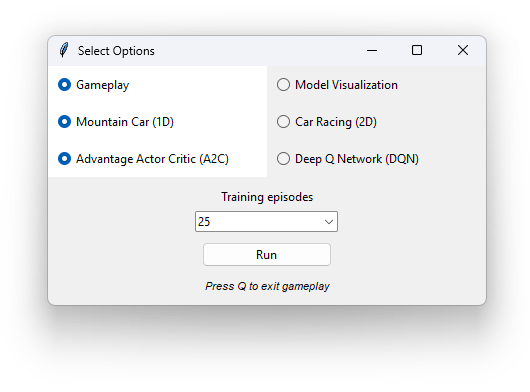
\includegraphics[width=0.45\textwidth]{figures/images/gui.png}
  \caption[Visualization GUI]{Graphical user interface for accessing the visualization suite}
  \label{fig:gui}
\end{figure}


In \autoref{fig:mountain_car_gui}, we can see the visualizations for Mountain
Car. On the left, have a visualization of the reward history graph with a
slider to control the rolling average window size. On the right, we have both a
weight distribution histogram and node connection graph side by side. The
slider below controls which model to use for the graphs, based on the number of
training episodes.

\autoref{fig:car_racing_gui} shows the Car Racing visualization GUI. Similarly to the Mountain Car visualization, we have a reward history graph. This works in exactly the same way as described above, as it is using the same runner file to load the GUI, with different data. The difference lies in the model visualization, where we can see the filters of the first layer of the CNN instead.

The GUI dynamically updates to reflect the changes in the graphs when either of
the sliders is used.

\begin{figure}[H]
  \centering
  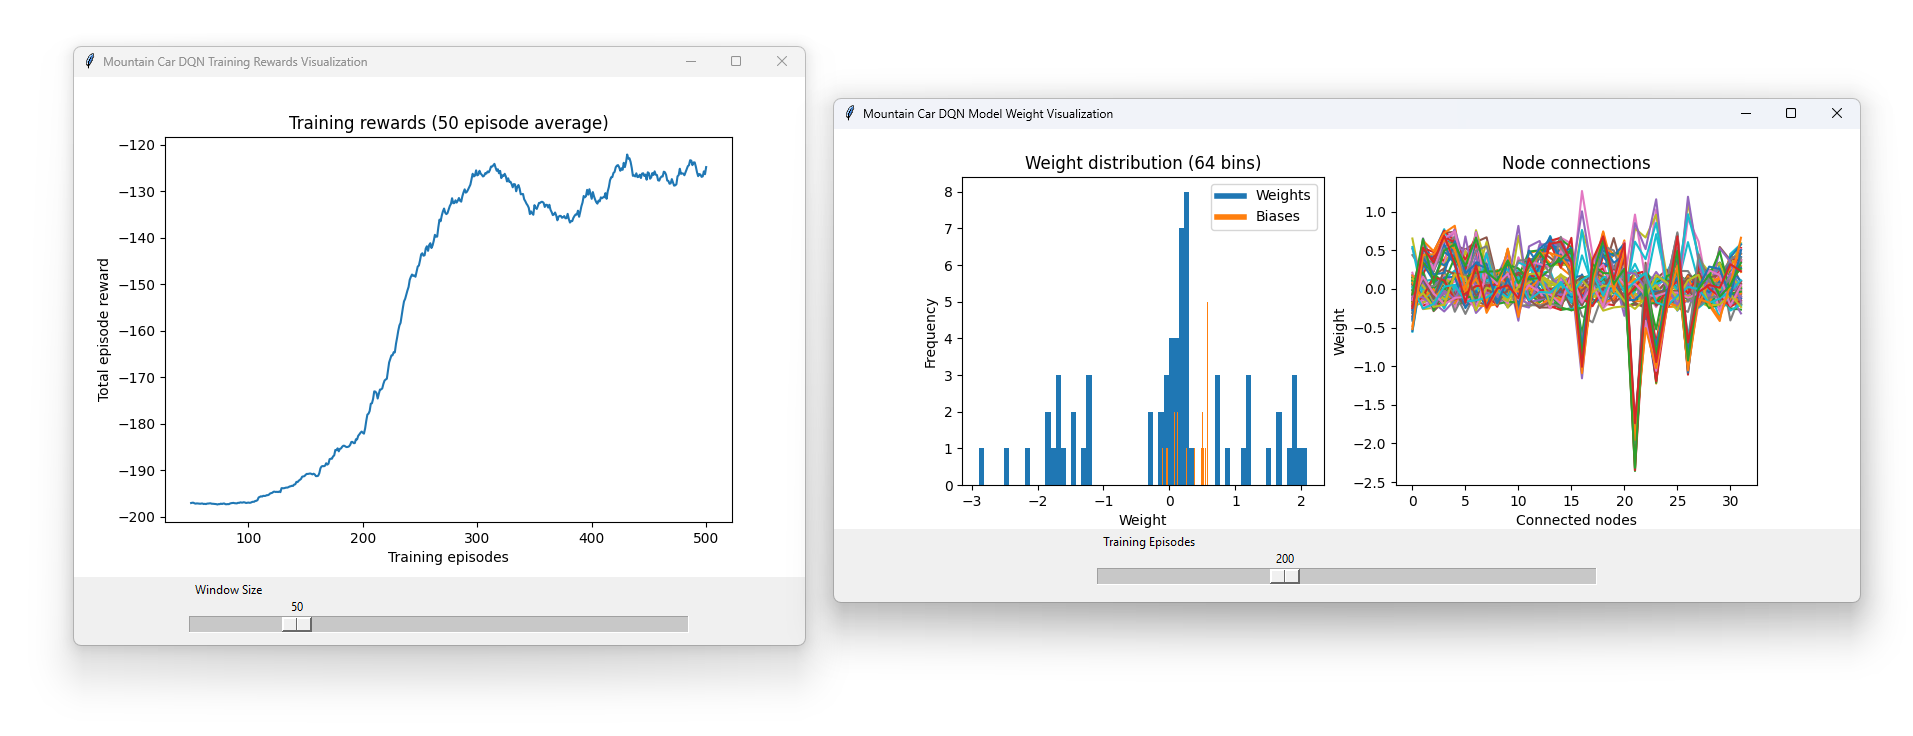
\includegraphics[width=1\textwidth]{figures/images/mountain_car_gui.png}
  \caption[Mountain Car DQN model visualization GUI]{Model visualization GUI for Mountain Car DQN}
  \label{fig:mountain_car_gui}
\end{figure}


\begin{figure}[H]
  \centering
  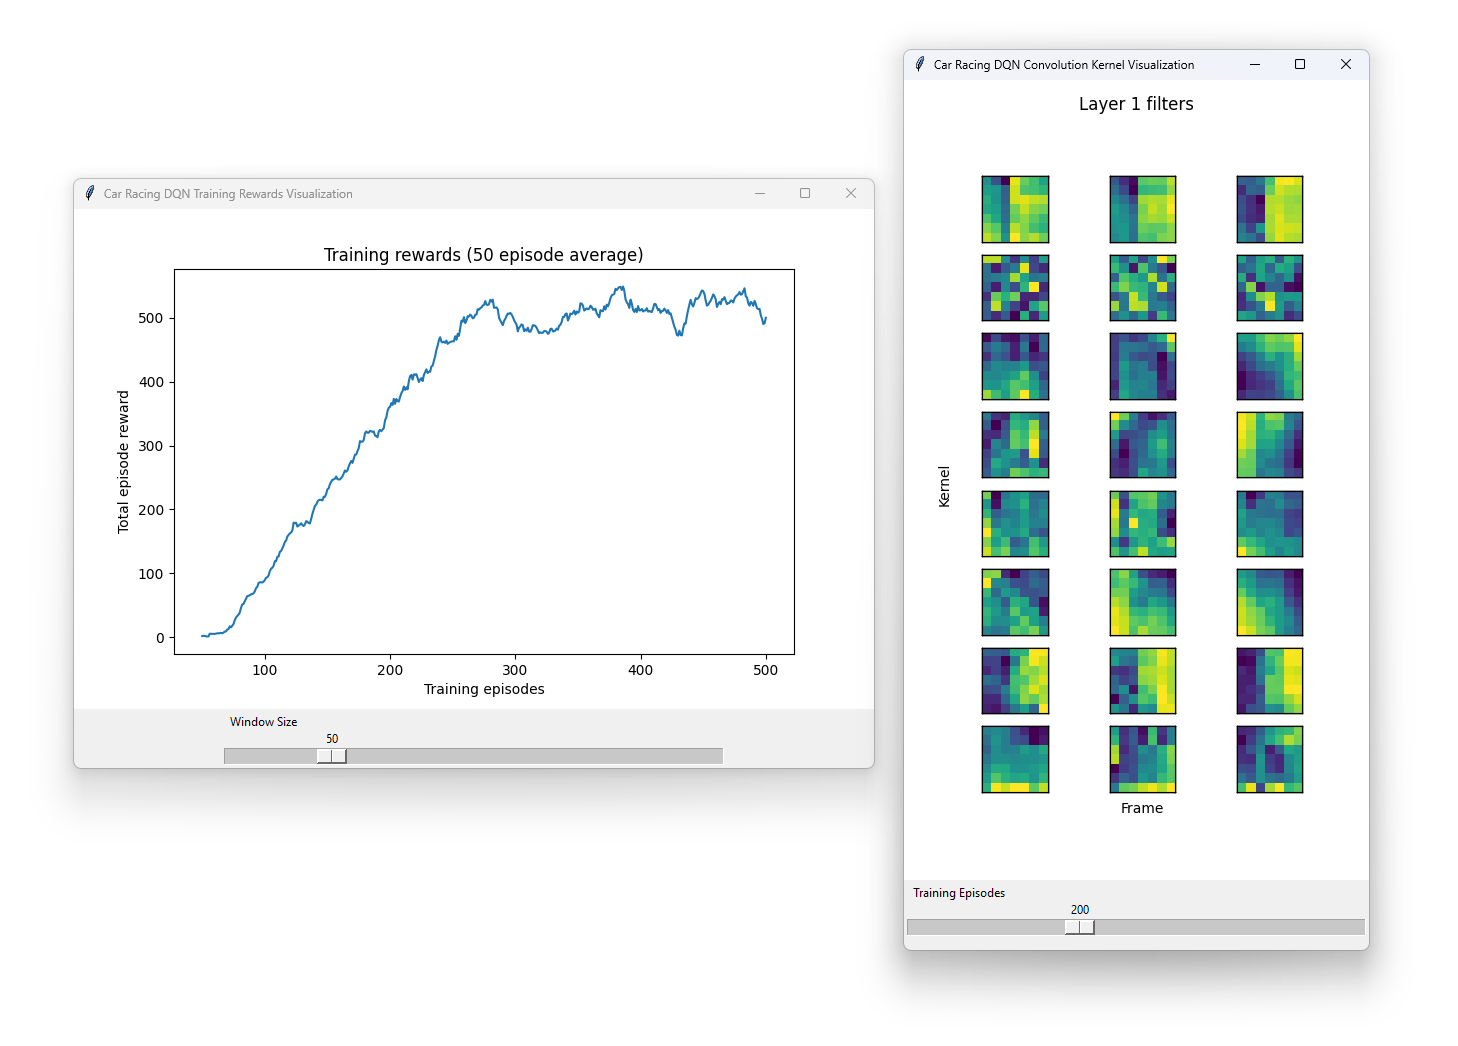
\includegraphics[width=0.8\textwidth]{figures/images/car_racing_gui.png}
  \caption[Car Racing DQN model visualization GUI]{Model visualization GUI for Car Racing DQN}
  \label{fig:car_racing_gui}
\end{figure}


\chapter{Experimentation \& Evaluation}
This chapter focuses on the evaluating the experiments with each agent, and the
results obtained doing so. We analyse the reasoning behind the results, and
propose potential mechanisms to improve them. The architecture of the neural
networks was kept relatively constant throughout the process, as this was not
the basis of the experiments.

\section{Hyperparameter Selection}

Due to the hyperparameter sensitivity of the deep Q-network (DQN) and the
advantage actor-critic (A2C) algorithm, paired with the long training time for
the agents, experimentation required a wealth of thought and effort channeled
precisely towards the correct direction. As mentioned in the abstract, the aim
of this project was to reduce training time, so we make comparisons using the
results after training the agents for 500 episodes. All of the hyperparameters
used in the algorithms are provided in \autoref{chp:hyperparameters}.

The learning rates for the all of the networks except the Car Racing A2C were
kept at $1\times 10^{-3}$; this value was found to produce relatively fast
convergence without compromising too much on the stability. For the Car Racing
A2C agent, this value was found to be too high; the agent would quickly
converge to the "gas" for all of the states as a "master action", so the
learning rate was set to $1\times 10^{-5}$.

A critical hyperparameter for the deep Q-learning algorithm was the
$\epsilon$-decay multiplier; we found that a value of 0.99 struck the balance
between enough exploration, while still allowing the agent to exploit its
discovered strategies enough within 500 episodes.

Although it has been found that large batch sizes improve training performance
\cite{stooke2018accelerated}, this would require high end compute resources,
especially a lot of memory and CPU cache. Due to this constraint, we found the
maximum batch size of 32 for the deep Q-learning algorithm to be high enough to
train the agent without negatively impacting quality substantially, while being
low enough to not crash the training machine due to excessive resource usage.

\begin{table}[H]
  \centering
  \begin{tabular}{|c|c|c|c|}
    \hline
    \multicolumn{2}{|c|}{\multirow{2}{*}}                        & \multicolumn{2}{c|}{\textbf{Game}}                                                                             \\
    \cline{3-4}
    \multicolumn{2}{|c|}{\multirow{-2}{*}{\textbf{Score Table}}} & \textbf{Mountain Car}                                                & \textbf{Car Racing}                     \\
    \hline
    \multirow{4}{*}{\textbf{Agent}}
                                                                 & \textbf{Random}                                                      & $-200\pm 0$         & $-65\pm 6$        \\
                                                                 & \textbf{DQN}                                                         & $-137\pm21$         & $\bm{623\pm 182}$ \\
                                                                 & \textbf{A2C}                                                         & $\bm{-135\pm 32}$   & $-17\pm 47$       \\
                                                                 & \textbf{Research} \cite{hernandez2019understanding, ha2018recurrent} & $-151 \pm 18$       & $343 \pm 18$      \\
    \hline
  \end{tabular}
  \caption[DQN and A2C testing results]{Average rewards after 500 episodes of training (1000 episode testing mean). The highest score for each game is in \textbf{bold}.}
  \label{table:results}
\end{table}


\section{Mountain Car}

\subsection{Model Evaluation}

As we can see from the rolling mean reward graph in
\autoref{fig:mountain_car_rewards}, both algorithms start to converge to a
solution by 500 episodes. A2C initially learns much quicker than the DQN, but
the DQN catches up by 450 episodes.

\begin{figure}[H]
  \centering
  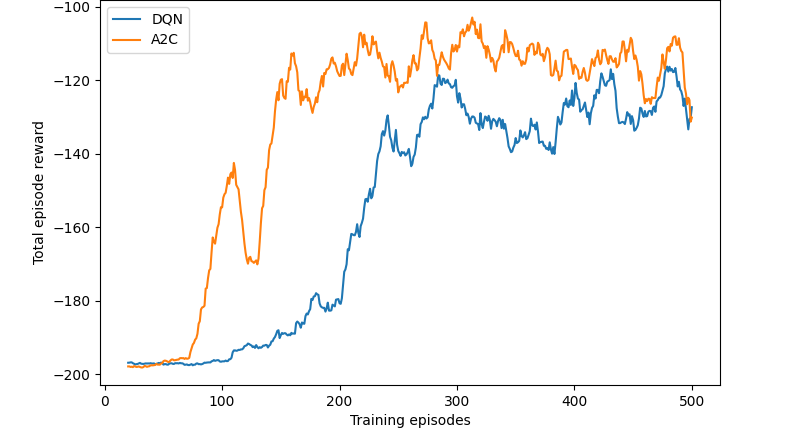
\includegraphics[width=0.75\textwidth]{figures/images/mountain_car_rewards.png}
  \caption[Mountain Car training rewards]{Mountain Car training rewards for DQN and A2C agents, with 20 episode rolling average}
  \label{fig:mountain_car_rewards}
\end{figure}


The first column in \autoref{table:results} shows the average scores for the
Mountain Car agents with 1000 test episodes; both of the algorithms perform
extremely similarly in terms of raw score. They both greatly outperform both
the research value and random action\footnote{This is the score of an agent
  that chooses completely random actions} value by over 13 points, which equates
to approximately a 9\% improvement in score. The standard deviation in the
score for the DQN agent is very similar to the research value; the same can not
be said about the A2C agent, which displays approximately a 50\% higher
standard deviation compared to the research and DQN values. This indicates that
the DQN is more confident in its policy, while the A2C is much less stable.

\subsection{Visualization Evaluation}
For Mountain Car, the visualization presents a histogram of the neural
network's weights as shown in \autoref{fig:mountain_car_w_viz}, and a line
graph with the weights values from one node to all of it's connected nodes as
shown in \autoref{fig:mountain_car_n_viz}. These are the middle layer's weights
for the deep Q-network and the A2C's actor network. They can be controlled
using a slider, to use a snapshot of the network at the selected the number of
training episodes. In \autoref{fig:mountain_car_w_viz} and
\autoref{fig:mountain_car_n_viz}, we can see the progression of the neural
network from 25 training episodes to 500; the network's improvement is clear,
from randomly selecting actions as the weights are relatively uniformly spread,
to wider distribution of a few weights with a high density of weights around 0
indicating learned features.

\begin{figure}[H]
  \captionsetup[subfigure]{justification=centering}
  \centering
  \begin{subfigure}[t]{0.47\linewidth}
    {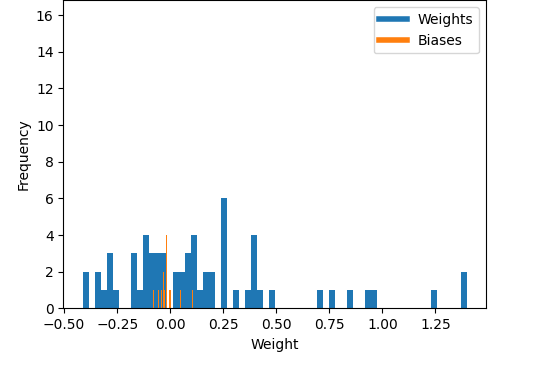
\includegraphics[height=5cm]{figures/images/mountain_car_weights_25.png}}
    \caption{After 25 episodes}
  \end{subfigure}
  \hfill
  \begin{subfigure}[t]{0.47\linewidth}
    {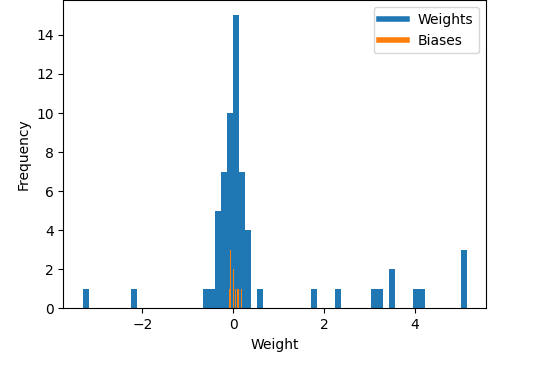
\includegraphics[height=5cm]{figures/images/mountain_car_weights_500.png}}
    \caption{After 500 episodes}
  \end{subfigure}
  \caption{Mountain Car weight distribution graphs}
  \label{fig:mountain_car_w_viz}
\end{figure}


\begin{figure}[H]
  \captionsetup[subfigure]{justification=centering}
  \centering
  \begin{subfigure}[t]{0.47\linewidth}
    {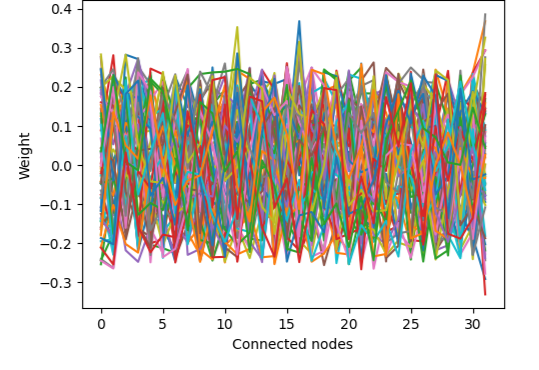
\includegraphics[height=5cm]{figures/images/mountain_car_nodes_25.png}}
    \caption{After 25 episodes}
  \end{subfigure}
  \hfill
  \begin{subfigure}[t]{0.47\linewidth}
    {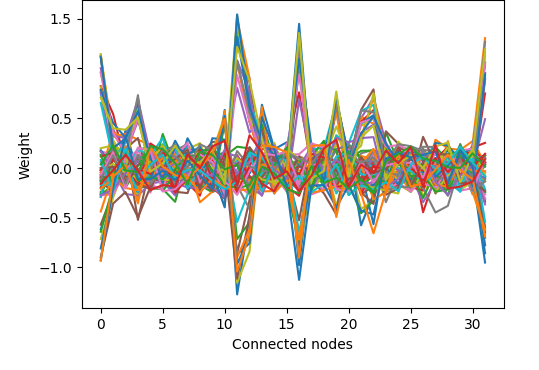
\includegraphics[height=5cm]{figures/images/mountain_car_nodes_500.png}}
    \caption{After 500 episodes}
  \end{subfigure}
  \caption{Mountain Car node connection graphs}
  \label{fig:mountain_car_n_viz}
\end{figure}


\subsection{Gameplay Findings}

Viewing the gameplay indicated which actions the agents were taking; it was
observed that both agents would accelerate too much towards the left and bump
into the environment boundary, instead of reversing acceleration earlier on the
hill. This is likely a result of the reward shaping function defined in
\autoref{sec:reward_shaping}, as it always promotes increasing speed without
consideration for the agent's position. An optimization would be a more nuanced
reward function, that for example disincentivizes speeds over a certain
threshold when the agent's state is on the left hill.

\subsection{Catastrophic Forgetting}

At around 100 episodes, the A2C agent's score suddenly drops by a substantial
amount, as we can see in \autoref{fig:mountain_car_rewards}. This is likely due
to the phenomenon of catastrophic forgetting \cite{parisi2019continual}, which
happens because the agent drastically updates the weights in the network when
learning a new strategy because of exploring new experiences. Mitigating this
issue could involve an approach such as implementing progressive neural
networks \cite{rusu2016progressive} or dynamic self-organizing maps
\cite{lo2019overcoming}.

\subsection{Exploration Action Probabilities}

A major revelation for the DQN agent was setting a custom probability
distribution for the $\epsilon$-greedy exploration; instead of sampling the
action from a uniform distribution, we specified an array with the probability
for each action which allowed exploration to be biased towards actions that
usually lead to higher rewards; in this case, that is the "left" and "right"
actions rather than doing nothing. We can find the custom probability
distribution for the Mountain Car actions in
\autoref{table:mountain_car_dqn_probs}.

\begin{table}[H]
  \centering
  \begin{tabular}{|c|c|c|c|c|c|c|}
    \hline
    \textbf{Action}      & Left & Nothing & Right \\
    \hline
    \textbf{Probability} & 0.4  & 0.2     & 0.4   \\
    \hline
  \end{tabular}
  \caption{Mountain Car DQN action probabilities} \label{table:mountain_car_dqn_probs}
\end{table}


Since we are not using an $\epsilon$-greedy policy for the advantage
actor-critic algorithm, the same distribution could not be applied to it.

\section{Car Racing}

\subsection{Model Evaluation}

The complexity of this environment posed a challenge to both of the algorithms,
though the A2C agent struggled more to start converging to a policy; as we can
see in \autoref{fig:car_racing_rewards}, the DQN just starts to converge by the
end of the 500 training episodes, as the variation in episode rewards starts to
decrease slowly. However, the A2C agent is severely lagging behind; it was
trained for longer to ensure there wasn't a fault in the algorithm, and it
started improving in performance by 750 episodes.

\begin{figure}[H]
  \centering
  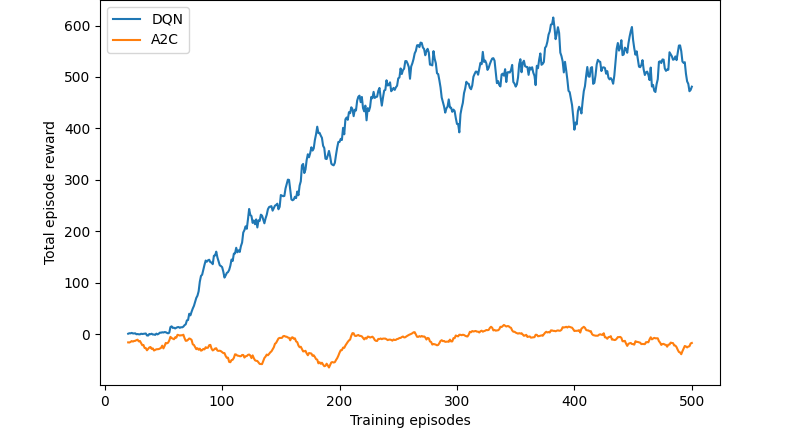
\includegraphics[width=0.75\textwidth]{figures/images/car_racing_rewards.png}
  \caption[Car Racing training rewards]{Car Racing training rewards for DQN and A2C agents, with 20 episode rolling average}
  \label{fig:car_racing_rewards}
\end{figure}


The second column in \autoref{table:results} shows the average scores for the
Car Racing agents with 1000 test episodes; the DQN agent far outperforms all of
the other agents, including the A2C agent, the research value and the random
action value. It must also be noted that the standard deviation for the DQN
agent is far higher than any of the others, indicating that the training is
still very unstable, and that the agent hasn't fully converged to an optimal
Q-function. Looking at final scores, the DQN agent outperforms the research
value approximately 86\%; while the A2C agent doesn't reach this score within
500 episodes, it performs as well as the DQN agent after 1000 episodes.

One reason why the A2C algorithm takes longer to converge could be due to the
one-step nature of the algorithm. We define a custom reward function for
Mountain Car, so it's not a problem in that environment, but one-step lookahead
severely limits the capability of Car Racing agent. The benefit to looking
ahead further to compute the expected return is that it would allow the agent
to make moves based on longer term changes in the track, such as a corner "out
of sight" for the one-step algorithm.

\subsection{Visualization Evaluation}
For Car Racing, the visualization shows the progression of the filters from the
first convolution layer of the network; in the case of the A2C agent, it shows
the actor's filters. In \autoref{fig:car_racing_filter_viz}, we can see the
change in the CNN filters; the vertical axis represents the filter, and the
horizontal represents which frame in the frame stack the filter corresponds to.
While slightly less informative than the visualization for Mountain Car, it is
still indicative of the change in the filters after training. We can also see
these filters applied to a frame of the game, in
\autoref{fig:car_racing_frame_viz}; this shows the filters' corresponding
feature maps\footnote{Note that the feature map visualization was not included
  in the final code submission}, where the road is clearly distinguished from the
rest of the image. Similarly to the Mountain Car visualization, a slider can be
used to select the number of episodes to determine which neural network to use.

\begin{figure}[H]
  \captionsetup[subfigure]{justification=centering}
  \centering
  \begin{subfigure}{0.44\linewidth}
    {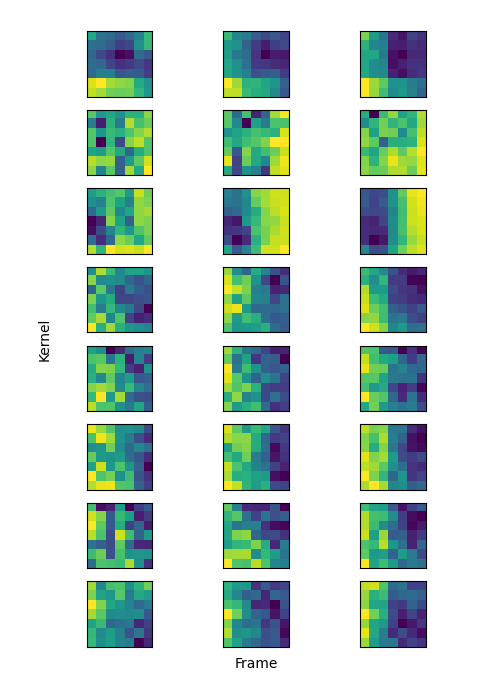
\includegraphics[height=9cm]{figures/images/car_racing_filters_25.png}}
    \caption{After 25 episodes}
  \end{subfigure}
  \hfill
  \begin{subfigure}{0.44\linewidth}
    {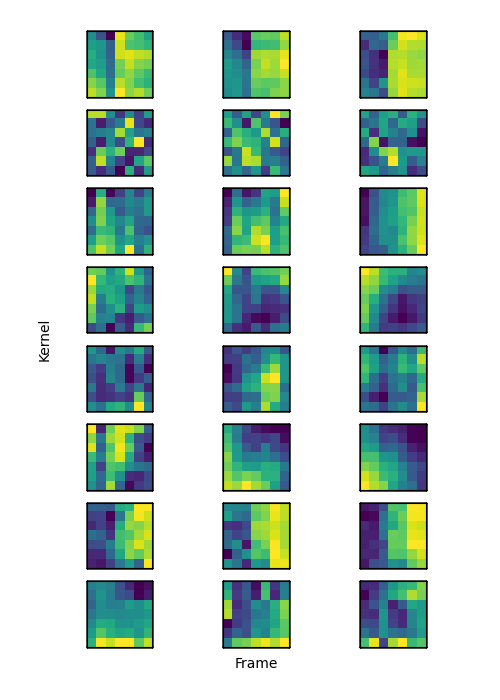
\includegraphics[height=9cm]{figures/images/car_racing_filters_500.png}}
    \caption{After 500 episodes}
  \end{subfigure}
  \caption[Car Racing filter plots]{Car Racing layer 1 filter plots}
  \label{fig:car_racing_filter_viz}
\end{figure}


\begin{figure}[H]
  \captionsetup[subfigure]{justification=centering}
  \centering
  \begin{subfigure}{0.44\linewidth}
    {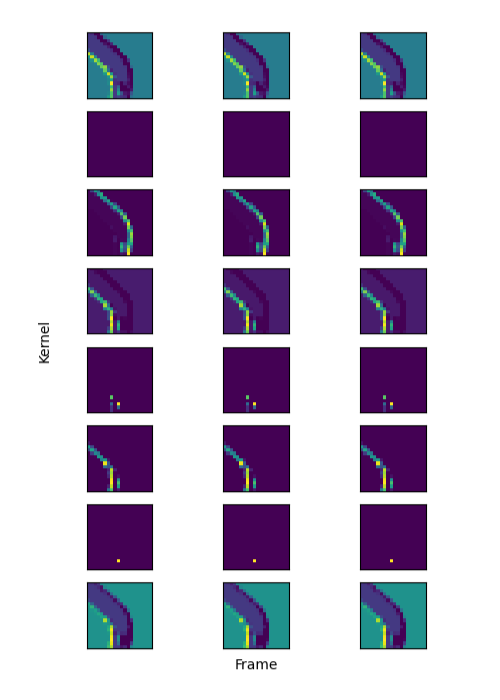
\includegraphics[height=9cm]{figures/images/car_racing_frames_25.png}}
    \caption{After 25 episodes}
  \end{subfigure}
  \hfill
  \begin{subfigure}{0.44\linewidth}
    {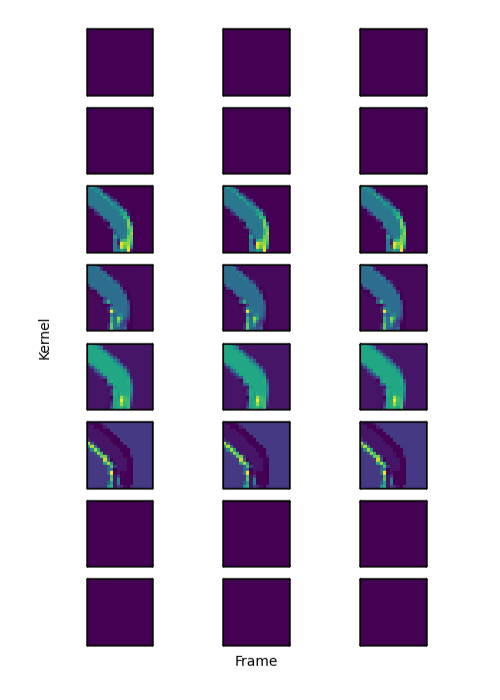
\includegraphics[height=9cm]{figures/images/car_racing_frames_500.png}}
    \caption{After 500 episodes}
  \end{subfigure}
  \caption[Car Racing feature map plots]{Car Racing layer 1 feature map plots}
  \label{fig:car_racing_frame_viz}
\end{figure}


\subsection{Gameplay Findings}
The gameplay for Car Racing was very insightful; as training progressed, the
agents learned to cut sharp corners, but they also started to very slowly veer
off the edge of the track, losing points. The main reason the agents couldn't
complete the track was spinning out of control, and they would usually not
recover from this. They would end up on a part of the environment with only
grass, or if they found their way back to the track, they would not know which
way was forward as there is no indication of direction in the environment. This
can be mitigated by training for more than 500 episodes, as the agents would
reach a more stable and optimal policy.

\subsection{Negative Reward Break}
A major finding during experimentation was that the episodes would last
extremely long, with the agent's consistently losing points, especially in the
early stages of training. To mitigate this issue, a negative reward break was
implemented. If the agent receives a negative reward consecutively for a
threshold number of steps, the episode is terminated.

A threshold value of 100 was found to provide a balance between the episodes
not lasting too long, and the agent learning to recover from minor errors that
would result in a few steps of consecutive negative rewards.

\subsection{Exploration Action Probabilities}
Similarly to the DQN used for Mountain Car, biasing the agent towards certain
actions helped in the training speed of the algorithm. The car benefits from
exploring the "gas" action the most, which is expected as it needs to move
forward to pass more tiles on the track. We can find the custom probability
distribution for the Car Racing actions in
\autoref{table:car_racing_dqn_probs}.

\begin{table}[H]
  \centering
  \begin{tabular}{|c|c|c|c|c|c|c|}
    \hline
    \textbf{Action}      & Nothing & Left & Right & Gas & Brake \\
    \hline
    \textbf{Probability} & 0.0     & 0.2  & 0.2   & 0.5 & 0.1   \\
    \hline
  \end{tabular}
  \caption{Car Racing DQN action probabilities}
  \label{table:car_racing_dqn_probs}
\end{table}


\subsection{Frame Skipping}
With the highly dynamic and fast-paced nature of this environment, the commonly
used value in research of skipping $n = 3$ frames \cite{bellemare2013arcade}
turned out to be too high; the agent would go off course by repeating the same
move for too long, due to the high speed of the car. A value of skipping $n =
  2$ frames yielded the optimal balance between reducing correlative frame data
without overextending the single chosen action. Note that reward was still
measured for the skipped frames, and used by the agent in training the
networks.

\chapter{Conclusion}

\section{Achievements}
We have successfully achieved our goals for this project; we have shown the
vast improvement that domain specific techniques such as input preprocessing,
negative reward breaks, custom exploration action probabilities and reward
shaping can bring to advantage actor-critic and deep Q-learning techniques. We
achieved over 9\% improvement in score for the Mountain Car environment and
86\% improvement in score for the Car Racing environment, within 500 episodes
for three agents and 1000 episodes for the fourth. We have also shown the
benefit of a robust visualization system in helping with the fine tuning of our
neural network's hyperparameters.

This project has been very insightful in terms of researching, understanding,
and optimizing a range of reinforcement learning algorithms, and their
applications to game playing environments; I have learned a great deal about
reinforcement learning and its constantly expanding capabilities.

\section{Limitations}

Any project would not be complete without its weaknesses, and this project is
no different. A major finding from the experimentation was the limitation of
restricting training episodes; while we were successful in improving model
performance with the constraints, these results came with a cost to the
stability of the model, most prevalently but not exclusively to the Car Racing
deep Q-network.

We also needed more than 500 episodes to reach performance comparable to the
research values in Car Racing with the advantage actor-critic agent; this
clearly indicates room for improvement in the algorithm.

\newpage

\section{Future Work}

Improving reinforcement learning model stability is a key area of research to
allow these algorithms to be applied to more complex scenarios. Predictability
is of utmost importance in real world situations such as vision based
self-driving vehicles \cite{liang2018cirl, sallab2016end} and multi-robot path
planning \cite{yang2020multi}. This could be done using techniques such as
target networks with soft network updates \cite{lillicrap2015continuous},
stochastic weight averaging \cite{nikishin2018improving}, and gradient clipping
\cite{mai2021stability}.

Another area for future development could be to investigate the impact of
$n$-step advantage actor-critic algorithms, where $n$ is the primary
hyperparameter under test. The lack of direct research in this field makes it
an excellent topic for further investigation.

Looking beyond the scope of this project, the recent proposals of using quantum
agents in reinforcement learning through techniques such as quantum Q-learning,
which uses parametrized quantum circuit instead of traditional neural networks
\cite{skolik2022quantum}, are an extremely thrilling prospect which I intend to
pursue in the near future.

\nocite{*}

\printbibliography[notkeyword={fig}, heading=bibintoc, title={References}]
\printbibliography[keyword={fig}, heading=bibintoc, title={References for Figures}]
\appendix
\chapter{Training Hyperparameters} \label{chp:hyperparameters}
\subsection*{Mountain Car DQN}
\begin{itemize}
  \item \textbf{Episodes} -- 500
  \item \textbf{Learning rate} -- $1 \times 10^{-3}$
  \item \textbf{$\gamma$} -- 0.99

  \item \textbf{$\epsilon$ initial value} -- 1.00
  \item \textbf{$\epsilon$ decay multiplier} -- 0.99
  \item \textbf{$\epsilon$ minimum} -- 0.01
  \item \textbf{Action probabilities} -- $[0.4, 0.2, 0.4]$ for $\left[\text{left}, \text{nothing},
            \text{right}\right]$

  \item \textbf{Batch size} -- 32
  \item \textbf{Replay buffer size} -- 100000
\end{itemize}

\subsection*{Mountain Car A2C}
\begin{itemize}
  \item \textbf{Episodes} -- 500
  \item \textbf{Learning rate} -- $1 \times 10^{-3}$
  \item \textbf{$\gamma$} -- 0.99
\end{itemize}

\newpage

\subsection*{Car Racing DQN}
\begin{itemize}
  \item \textbf{Episodes} -- 500
  \item \textbf{Learning rate} -- $1 \times 10^{-3}$
  \item \textbf{$\gamma$} -- 0.95

  \item \textbf{Frame skip} -- 2
  \item \textbf{Frame stack size} -- 3
  \item \textbf{Negative reward break} -- 100

  \item \textbf{$\epsilon$ initial value} -- 1.00
  \item \textbf{$\epsilon$ decay multiplier} -- 0.99
  \item \textbf{$\epsilon$ minimum} -- 0.01
  \item \textbf{Action probabilities} -- $[0.0, 0.2, 0.2, 0.5, 0.1]$ for $\left[\text{nothing},
            \text{left}, \text{right}, \text{gas}, \text{brake}\right]$

  \item \textbf{Batch size} -- 32
  \item \textbf{Replay buffer size} -- 5000
\end{itemize}

\subsection*{Car Racing A2C}
\begin{itemize}
  \item \textbf{Episodes} -- 500
  \item \textbf{Learning rate} -- $1 \times 10^{-5}$
  \item \textbf{$\gamma$} -- 0.95

  \item \textbf{Frame skip} -- 2
  \item \textbf{Frame stack size} -- 3
  \item \textbf{Negative reward break} -- 100

  \item \textbf{Entropy coefficient} -- 0.1
\end{itemize}

\end{document}
